\documentclass[11pt, a4paper]{lecturenote}

\usepackage{rotating, tabularx}
\usepackage{threeparttable}

\begin{document}

\title{플랫폼 경제의 이해}
\author{이남형 \medskip\\{\normalsize 한국방송통신대학교 경제학과}}
\date{2021년 2학기 \medskip\\{\normalsize Ver. 1.02}}
\maketitle

\pagenumbering{roman} % 로마 숫자 페이지 매기기

\chapter*{알림}

이 강의안은 한국방송통신대학교, \textbf{플랫폼 경제의 이해} 수업을 위해 제작되었습니다.

%강의안에는 사진, 그래프 등을 이용한 설명이 없습니다. 이에 대한 내용은 강의 동영상과 강의 프리젠테이션을 함께 참고하여 공부하기 바랍니다.

오탈자, 오류, 개선사항 등은 이메일 $<$\href{mailto:namhyunglee@knou.ac.kr}{namhyunglee@knou.ac.kr}$>$ 또는 홈페이지 과목 상담 $<$\url{https://www.namhyunglee.net/questions/teachings/}$>$으로 연락주시기 바랍니다.

\begin{itemize}
\item 변경사항
	\begin{itemize}
	\item Ver. 1.02: 2021년 2학기
		\begin{itemize}
		\item \ref{cha:platforminlabormarket}장, ``하청 계약" $\rightarrow$ ``플랫폼 사용 약관 동의", 관련 정리하기 내용도 수정
		\end{itemize}
	\item Ver. 1.01: 2021년 2학기
		\begin{itemize}
		\item \ref{cha:ecommerce}장, ``B2C 시장이 21조 달러로 ... B2B 시장은 4.4조 달러" $\rightarrow$ ``B2B 시장이 21조 달러로 ... B2C 시장은 4.4조 달러", 관련 정리하기 내용도 수정
		\end{itemize}
	\item Ver. 1.0: 2021년 2학기
	\end{itemize}
\end{itemize}

\tableofcontents
\listoffigures
\listoftables
%\include{revision}



\pagenumbering{arabic} % 아라비아 숫자 페이지 매기기
\chapter{플랫폼 경제의 특징}\label{cha:whatisplatform}

\section*{학습개요}
플랫폼 경제의 특징을 설명하고, 매칭과 기술의 두 가지 성격으로 분류한다. 앞으로 배울 내용을 개관하며, 특히 다면(양면) 시장이론과 네트워크 효과와 이로 인한 플랫폼의 경제적 특성을 알아본다. 그리고 플랫폼의 사회적 특성으로서 과세, 반독점, 노동 이슈를 간략히 살펴본다.


\section*{학습목표}
\begin{enumerate}
\item 플랫폼의 특징을 설명할 수 있다.
\item 플랫폼이 최신 현상이 아님을 이해한다.
\item 인터넷 발달 이전과 이후 플랫폼에 나타난 변화를 설명할 수 있다.
\item 매칭 플랫폼과 기술 플랫폼의 특징과 수익 창출 방법을 설명할 수 있다.
\end{enumerate}

\section*{주요 용어}
플랫폼, 외부성, 수요의 가격 탄력성, 호환성, 기술 개방, 과세, 반독점, 주문형 노동


\pagebreak

\section{플랫폼의 기능과 분류}\label{sec:}
\begin{itemize}
\item 쇼핑몰, 신용카드, 텔레비전(신문), 닌텐도 게임기의 공통점은 무엇일까? \cite[pp. 991--992]{Rochet:2006jl}
	\begin{itemize}
	\item 상점 $\leftrightarrow$ 쇼핑몰 $\leftrightarrow$ 소비자
	\item 가맹점 $\leftrightarrow$ 신용카드 $\leftrightarrow$ 구매자
	\item 시청자 $\leftrightarrow$ 텔레비전 $\leftrightarrow$ 광고주
	\item 게임 개발사 $\leftrightarrow$ 게임기 제작사 $\leftrightarrow$ 게임 이용자
	\end{itemize}
\item 이들은 모두 플랫폼 \cite[p. 13]{Cusumano:2019aa} 
	\begin{quote}
	``서로 다른 종류의 사용자가 상호 활동할 수 있도록 만들어주는 것"
	\end{quote}
\item 경제학의 전통적인 관심
	\begin{itemize}
	\item 새로운 상품의 생산 $\rightarrow$ 더 낮은 가격으로 생산 $\rightarrow$ 운송 비용을 낮추어 더 효율적으로 교환
	\end{itemize}
\item 간과해온 질문: 판매자와 구매자는 어떻게 만나는가? \cite[p. 380]{Tirole:2017aa}
	\begin{itemize}
	\item 인터넷 이전: 제한된 상품과 서비스 카탈로그
		\begin{itemize}
		\item 음악을 듣기 위해서는 길거리에서 들리는 음악을 듣거나, 라디오나 TV에서 틀어주는 것을 듣거나
		\item 책을 읽기 위해서는 서점에 진열된 것을 보거나, 도서관에 소장된 것을 보거나
		\end{itemize}
	\item 인터넷 이후: 카탈로그의 길이가 무제한으로 늘어남
		\begin{itemize}
		\item $\rightarrow$ 무엇이 제공되고 있는지, 누구와 거래를 할 것인지 평가하는 것이 중요
		\item $\rightarrow$ 신호 비용(signaling costs)
		\item $\rightarrow$ 정보가 무한히 많으므로 중개인(플랫폼)을 두고 거래 상대방을 찾는 것이 효과적일 수 있음
		\end{itemize}
	\end{itemize}
\item 플랫폼의 첫 번째 유형: 매칭(matching) 플랫폼 \cite[p. 19]{Cusumano:2019aa}
	\begin{itemize}
	\item 플랫폼은 플랫폼 사용자에게 플랫폼에서 무엇을 제공하는지, 무엇이 가장 잘 맞는 지의 정보를 제공하는 것이 중요
	\item 공유 경제라고 불리는 비즈니스의 상당수가 여기에 해당
		\begin{itemize}
		\item 에어비앤비(Airbnb, 집), 우버(Uber, 차) 등
		\end{itemize}	
	\item 구글의 검색 엔진도 이 분류에 포함 \citep{Varian:2016vt}
		\begin{itemize}
		\item 검색자가 원하는 정보를 연결시켜주기 때문
		\end{itemize}
	\item 수익 창출
		\begin{itemize}
		\item 재화나 서비스의 판매 연결, 콘텐츠의 생산이나 공유 또는 광고 등
		\end{itemize}
	\end{itemize}
\item 플랫폼의 두 번째 유형: 기술(technological) 플랫폼
	\begin{itemize}
	\item 사용자 간 상호 작용을 가능하게 하는 기술적 기반(technical interface)을 제공
	\item 컴퓨터 운영체제(MS Windows, Apple MacOS, Linux 등), 모바일 기기 운영체제(Google Android, Apple iOS 등), 콘솔 게임기(Sony Playstation, MS Xbox, Nintendo 등) 등
	\item 수익 창출
		\begin{itemize}
		\item 재화나 서비스의 직접 판매 또는 대여, 보완재나 서비스의 개발 등
		\end{itemize}
	\end{itemize}
\item 혼합(Hybrid) 플랫폼? 
	\begin{itemize}
	\item 애플(Apple), 구글(Google): 모바일 기기 운영체제 $+$ 모바일 어플리케이션 판매
	\item 기업의 비즈니스를 중심으로 생각하면 가능한 분류. 하지만 분석을 위해 필요한 분류는 아님
	\end{itemize}
\end{itemize}

\section{플랫폼의 경제 이론}
\begin{itemize}
\item 다면 시장 이론(multi-sided market) \cite[pp. 383--388]{Tirole:2017aa}
	\begin{itemize}
	\item 플랫폼이 상대해야 하는 사용자를 면(side)으로 파악 $\rightarrow$ 기본은 양면 시장(two-sided market)
	\item 외부성과 수요의 가격 탄력성
		\begin{itemize}
		\item 외부성: 플랫폼의 사용자는 다른 어느 한 면의 활동으로부터 영향을 받음
			\begin{itemize}
			\item A면의 사용자가 B면의 상호 작용에서 더 많은 이득을 얻는다면, 플랫폼은 A면의 사용자에게 더 높은 이용료를 부과하고 B면의 사용자에게 상대적으로 낮은 이용료를 부과할 수 있음
			\item $\rightarrow$ 신문, 잡지, TV 등이 광고주로부터 돈을 받고, 독자나 시청자에게는 돈을 받지 않는지 설명 가능; 신용카드 회사가 가맹점으로부터만 수수료를 받고 구매자에게는 받지 않는 것도 설명 가능
			\end{itemize}
		\item 수요의 가격 탄력성: 가격 1퍼센트 상승으로 플랫폼이 몇 퍼센트의 소비자를 잃을 것인가를 보여줌 $\rightarrow$ 가격 결정의 기준
			\begin{itemize}
			\item 낮은 가격 탄력성: 가격을 높여도 수요 감소가 작으므로 수입이 증가할 수 있음
			\item 하지만, 이론적인 가능성일 뿐 $\rightarrow$ 소비자는 가격 상승에 대해 경쟁 플랫폼으로 옮길 수 있음
			\item $\rightarrow$ 신용카드 회사가 가맹점마다 수수료를 다르게 받는 이유를 설명 가능
			\end{itemize}	
		\end{itemize}
	\end{itemize}
\item 네트워크 이론(network theory)
	\begin{itemize}
	\item 네트워크와 네트워크 효과
		\begin{itemize}
		\item 네트워크: 노드(node)와 노드를 연결하는 링크(link)
		\item 네트워크 효과: 어떤 재화나 서비스를 사용하는 사람이 많아지면 많아질 수록 그 재화나 서비스의 가치가 더 커짐
		\item $\rightarrow$ 임계 질량(critical mass)과 승자 독식(winner takes all)
		\end{itemize}	
	\item 닭이 먼저일까 달걀이 먼저일까?
		\begin{itemize}
		\item 플랫폼은 B면의 사용자가 있기 전에 A면의 사용자 수가 충분하도록 투자할 필요가 있을 수 있음
		\item 게임기 제작사, 게임 사용자, 게임 개발사
			\begin{itemize}
			\item A 게임기의 사용자가 많지 않다면, 개발사는 A 게임기에서 작동하는 게임을 개발하지 않을 유인이 큼
			\item A 게임기 개발사는 게임 판매로 개발사가 얻는 수익을 시장 평균보다 더 높게 제시할 수 있음
			\item 동시에 A 게임기 개발사는 시장 평균 가격보다 낮은 가격으로 게임기를 판매하여 더 많은 소비자를 유인
			\item $\rightarrow$ 만약 A 게임기 개발사가 시장의 후발 주자라면, 성공적인 시장 진입을 위해 손해를 보면서 게임기를 판매할 수도 있음
			\end{itemize}
		\end{itemize}
	\item 호환성
		\begin{itemize}
		\item 소비자는 플랫폼을 선택할 수 있음 
		\item 플랫폼은 호환성을 위해 협조해야할까?
			\begin{itemize}
			\item 이동 통신에 대해서는 국가가 호환성을 강제
			\item 게임기, 신용카드 등은 강제가 아님
			\end{itemize}
		\item 플랫폼의 어떤 면(side)에서는 사용자가 다수의 플랫폼(multihoming) 또는 하나의 플랫폼(single homing)을 선택할 수 있음
			\begin{itemize}
			\item 여러 신용카드를 받는 가맹점 vs. 하나의 신용카드만 받는 가맹점
			\end{itemize}
		\end{itemize}
	\item 기술 개방
		\begin{itemize}
		\item 플랫폼은 여러 면의 경제 주체를 유인하기 위해 기술을 개방할 수도 개방하지 않을 수도 있음
		\item 모바일 기기 운영체제: 애플(Apple iOS) vs. 구글 안드로이드(Google Android)
		\end{itemize}
	\end{itemize}
\end{itemize}

\section{플랫폼 경제와 정책}
\begin{itemize}
\item 규제 
	\begin{itemize}
	\item 플랫폼에 대한 규제
		\begin{itemize}
		\item 과세: 국경을 초월한 기업 활동을 통한 수익을 어떻게 과세할 것인가?
		\item 반독점: 앞에서 본 것처럼 플랫폼은 양면에 비대칭적 가격 설정이 유리 $\rightarrow$ 전통적인 반독점 이론에서는 신규 기업의 시장 진입을 막는 약탈적 가격일 수 있음
			\begin{itemize}
			\item 하지만, 신규 진입 기업도 같은 전략을 사용할 것
			\item 과연 불공정 경쟁일까?
			\end{itemize}
		\end{itemize}
	\item 규제자로서의 플랫폼 $\rightarrow$ 플랫폼이 자선 사업가여서가 아니라 그렇게 하는 것이 유리하기 때문
		\begin{itemize}
		\item 판매자 간의 경쟁 촉진
		\item 가격 규제
		\item 품질 관리
		\item 정보 제공
		\end{itemize}
	\end{itemize}
\item 노동
	\begin{itemize}
	\item 주문형 노동
		\begin{itemize}
		\item 각종 대행(음식 배달, 쇼핑, 운전 등), 제시된 과업 수행 등
		\end{itemize}	
	\item 다수의 문제점 노출
		\begin{itemize}
		\item 불안정한 법적 지위와 낮은 소득
		\item 장시간 노동과 위험 감수
		\item 사회안전망으로부터의 사각 지대
		\end{itemize}
	\end{itemize}
\end{itemize}

\pagebreak

\section*{정리하기}
\begin{enumerate}
\item 경제학에서 정의하는 플랫폼은 "서로 다른 종류의 사용자가 상호 활동할 수 있도록 만들어주는 것"이다.
\item 플랫폼은 새로운 현상이 아니며, 쇼핑몰, 신용카드, (광고를 전달한다는 측면에서) 텔레비전/신문/라디오 등은 플랫폼의 속성을 갖고 있다.
\item 인터넷은 소비자가 확인할 수 있는 상품과 서비스의 목록을 크게 늘렸고, 이는 오히려 소비자가 원하는 정보를 찾고 평가해야하는 비용이 높아지는 상황을 초래했다. 따라서 플랫폼이 서로 원하는 거래 상대방을 찾아주는 것이 효과적일 수 있게 되었다.
\item 매칭 플랫폼은 플랫폼 사용자가 원하는 것을 추천, 제공하는 것이 일반적이다. 검색 엔진이 대표적인 서비스이다. 재화나 서비스의 판매 또는 이의 연결, 콘텐츠의 생산이나 공유 또는 광고 등을 통해 수익을 창출한다.
\item 기술 플랫폼은 플랫폼 사용자 간 상호 작용을 가능하게 하는 기술적 기반을 제공한다. 컴퓨터나 모바일 기기 등의 운영체제가 대표적이다. 재화나 서비스의 직접 판매 또는 대여, 보완재나 서비스의 개발을 통해 수익을 창출하는 것이 일반적이다. 
\end{enumerate}



\chapter{양면 시장 이론}\label{cha:twosidedmarketheory}

\section*{학습개요}
플랫폼 경제를 설명하는 대표적인 경제 이론은 다면 시장 이론이다. 이 강의에서는 그 중 가장 단순한 구조인 양면시장이론(two-sided market theory)을 학습한다.


\section*{학습목표}
\begin{enumerate}
\item 양면 시장의 정의를 설명할 수 있다.
\item 양면 시장에서의 시소 원칙을 설명할 수 있다.
\item 플랫폼의 회원제 요금과 사용량 연동 요금을 구별할 수 있다.
\item 수요의 가격 탄력성에 따라 플랫폼이 이윤을 극대화 할 수 있는 전략을 설명할 수 있다.
\item 주어진 상황에 따라 하나의 플랫폼만 사용하는 것과 다수의 플랫폼만 사용하는 것의 관계를 설명할 수 있다.
\end{enumerate}

\section*{주요 용어}
양면 시장, 시소 원칙, 수요의 가격 탄력성, 하나의 플랫폼 사용(single-homing), 다수의 플랫폼 사용(multi-homing), 병목을 향한 경쟁

\pagebreak

\section{양면 시장의 정의}\label{sec:}
\begin{itemize}
\item 가격 구조를 강조한 정의 \cite[pp. 664--665]{Rochet:2006jl} $\rightarrow$ 반독점 규제와 연결됨
	\begin{quote}
	``플랫폼이 동일한 양에 대해 시장의 한 면에 더 높은 가격을 부과하고 다른 면에는 낮은 가격을 부과함으로써, 거래량에 영향을 줄 수 있을 때 양면 시장이라고 할 수 있다. 즉, 가격 구조가 중요하고, 플랫폼은 양면 모두가 플랫폼에 머물러 있도록 가격 구조를 설계할 수 있어야만 한다.  만약 어느 최종 사용자가 실제 할당된 짐을 받아들이지 않고 떠날 수 있다면 단면 시장이다\footnote{A market if two-sided if the platform can affect the volume of transactions by charging more to one side of the market and reducing the price paid by the other side by an equal amount; in other words, the price structure matters, and platforms must design it so as to bring both sides on board. The market is one-sided if the end-users negotiate away the actual allocation of the burden.}."
	\end{quote}
	\begin{itemize}
	\item 두 종류의 사용자 집단 
		\begin{itemize}
		\item 거래 중개를 위해 플랫폼이 필요
		\item 플랫폼은 재화나 서비스를 두 사용자에게 동시에 제공
		\end{itemize}
	\item 두 집단 간의 간접적인 외부성
		\begin{itemize}
		\item 어느 한 면의 사용자 수가 증가하면, 다른 면의 사용자에게 이득이 발생
		\item 이 두 가지 특성만 생각하면, 직접 거래를 제외한 일상의 거의 모든 거래는 어느 정도 양면 시장의 속성을 가짐
		\item 하지만, 양면 시장이라고 부를 수 있는 독특한 특징은 다음의 가격 구조
		\end{itemize}
	\item 비대칭적인 가격 구조
		\begin{itemize}
		\item 어느 한 면의 가격을 높이고 다른 한 면의 가격을 낮추기 때문
		\item 양면 모두가 플랫폼에 참여하도록 설계해야 함
		\item 동시에, 즉 양면 모두가 자신의 요금 체계를 받아들여야 함
		\end{itemize}
	\end{itemize}
\end{itemize}

\pagebreak

\section{양면 시장의 가격 결정}
\begin{itemize}
\item 가격 구조에 관한 질문
	\begin{enumerate}
	\item 가격 구조에 영향을 미치는 요소는 무엇인가? 
		\begin{itemize}
		\item \cite{Rochet:2006jl}, 시소 원칙(the Seesaw principle)
			\begin{itemize}
			\item 플랫폼의 이윤을 높이도록 A면에 높은 가격을 부과하게 하는 요인은, 더 높은 이윤을 얻고자 B면의 사용자를 유인하기 위해 B면의 가격을 낮추도록 할 수 있음
			\end{itemize}
		\item \href{https://news.naver.com/main/read.nhn?mode=LSD&mid=sec&sid1=105&oid=143&aid=0000044770}{김준엽, 2006, ``소니 PS3 1대 팔때마다 22만원씩 밑진다", 국민일보 2006.11.20.}	
			\begin{itemize}
			\item 게임 이용자 -- 콘솔 게임기 판매사 -- 게임 개발사
			\item  $\rightarrow$ 게임 이용자가 지불할 가격을 낮추면, 
			\item $\rightarrow$ 게임 이용자의 콘솔 게임기 수요와 게임 수요를 모두 늘릴 수 있음
			\item $\rightarrow$ 게임 개발사로부터의 로열티를 높일 수 있음
			\end{itemize}

				\begin{table}[htp]
				\begin{center}
				\begin{threeparttable}
				\caption{플랫폼 가격 전략의 예}
				\label{tab:moneyandsubsidysidesforcommonmultisdedplatformindustries}
				\begin{tabularx}{\textwidth}{lll}
				\toprule
				플랫폼 & A 면 & B면 \\
				\midrule
				콘솔 게임기 & 소비자는 한계 비용 또는  & 게임 개발사로부터 로열티를 받음 \\
				& 그 이하의 가격으로 콘솔 게임기를 구입 &   \\
				TV 방송 & 시청자의 지불은 없음 & 광고주로부터 광고비를 받음  \\
				신용카드 & 소비자의 지불은 없음,   & 가맹점으로부터 거래 수수료를 받음 \\
				& 마일리지, 포인트 등을 받기도 함 & \\
				쇼핑몰 & 소비자의 지불은 없음, & 판매점으로부터 임대료를 받음 \\
				& 무료 주차나 이벤트 등의 보상이 있기도 함 & \\
				온라인 쇼핑몰 & 소비자의 지불은 보통 없음  & 판매자가 수수료를 지불\\
				\bottomrule
				\end{tabularx}
				\begin{tablenotes}
				\small
				\item 출처: \cite{Evans:2017uw}, 표 2-1.
				\end{tablenotes}
				\end{threeparttable}
				\end{center}
				\end{table}%
			
		\end{itemize}

\pagebreak
		
	\item 플랫폼이 설계할 수 있는 가격 구조는 무엇인가?
		\begin{itemize}
		\item  전체 서비스에 대한 구독 요금을 지불 $\rightarrow$ 회원제 요금
		\item 매 거래마다 요금을 지불 $\rightarrow$ 사용량 연동 요금
		\item 이 두 방법이 상호 배타적이지는 않음
			\begin{itemize}
			\item	 즉, 동시에 존재하는 요금제도 있음
			\item 디지털 콘텐츠의 정기 구독 $+$ 특정 콘텐츠는 개별 구매
			\end{itemize}
		\end{itemize}
	\end{enumerate}
\item 두 가지 질문 모두와 관련하여, 현실적으로 중요한 이슈는 고려 대상이 되는 면에서의 수요의 가격 탄력성 \cite[pp. 129--130]{Rysman:2009aa}
	\begin{itemize}
	\item A 면의 가격 탄력성이 매우 높고, B 면의 가격 탄력성이 높지 않다면
	\item A 면에 한계비용보다 낮은 가격을 부과하여 더 많은 소비자를 유인하고, B 면은 한계비용보다 더 높은 가격을 부과(a higher mark-up pricing)할 수 있음
	\end{itemize}		
\item $\rightarrow$ 만약 A 면의 소비 증가로 B 면의 사용자를 더 유인할 수 있다면(즉, 간접적인 네트워크 효과가 있다면), 플랫폼은 양면 모두에서 이윤을 얻을 수 있음	
	\begin{itemize}
	\item 플랫폼은 A면 (왼쪽 그래프)과 B면(오른쪽 그래프) 모두를 상대

		\begin{figure}[htbp]
		\begin{center}
		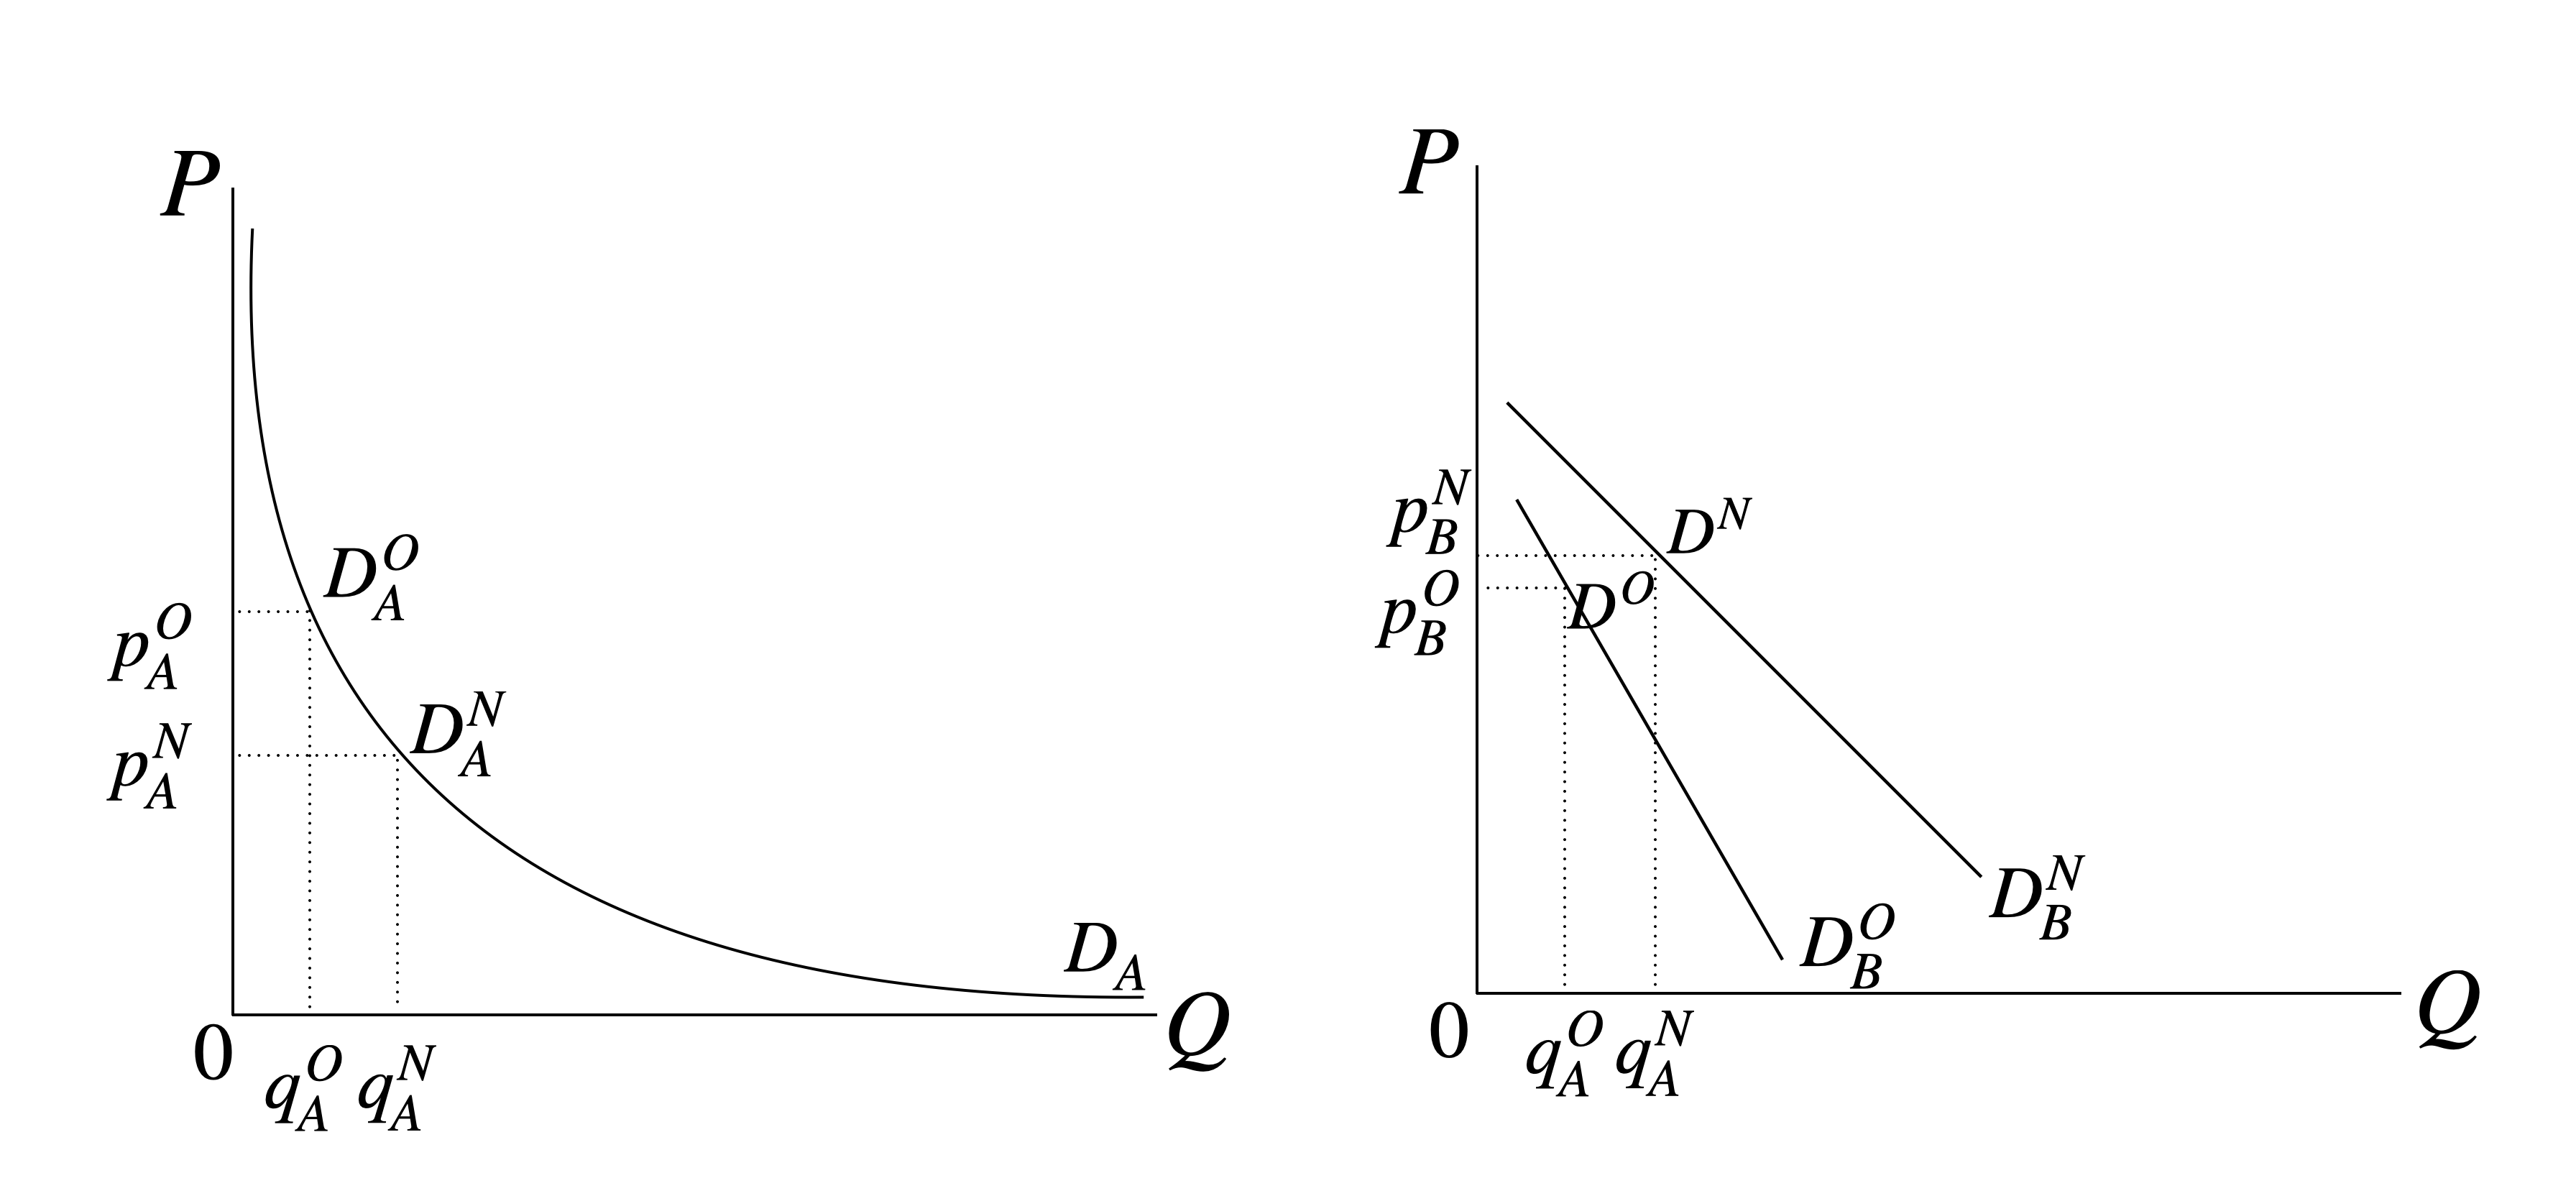
\includegraphics[scale=0.2]{two-sided-market-pricing.png}
		\caption{양면 시장의 가격 구조}
		\label{fig:two-sided-market-pricing}
		\end{center}
		\end{figure}
	
	\item 플랫폼이 A 면의 가격을 낮추면 ($p_{A}^{O} > p_{A}^{N}$), 수요량은 증가 ($q_{A}^{O} < q_{A}^{N} $)
		\begin{itemize}
		\item 수요량이 충분히 늘어나면, 수입이 증가 ($p_{A}^{O} q_{A}^{O} = \pi_{A}^{O} < \pi_{A}^{N} = p_{A}^{N} q_{A}^{N}$) 
		\end{itemize}
	\item 그리고, A 면의 수요량 증가로, B 면의 수요가 늘어나면 ($D_{B}^{O} \rightarrow D_{B}^{N}$)
	\item B 면에서 가격을 높여도 ($p_{B}^{O} < p_{B}^{N} $)
		\begin{itemize}
		\item 수입이 증가 ($p_{B}^{O} q_{A}^{O} = \pi_{B}^{O} < \pi_{B}^{N} = p_{B}^{N} q_{A}^{N}$)
		\item 즉, B면에서 사각형 $p_{B}^{O}0q_{A}^{O}D^{O}$의 면적보다 사각형 $p_{B}^{N}0q_{A}^{N}D^{N}$의 면적이 더 크다는 의미, A면도 마찬가지
		\end{itemize}
	\item 사각형 면적을 결정하는 것은 A면과 B면의 가격에 대한 수요 탄력성	
	\end{itemize}
\item $\rightarrow$ 플랫폼은 어느 한 면의 가격을 낮추고($\downarrow$), 다른 한 면의 가격을 높임으로써($\uparrow$) 이윤을 극대화 할 수 있음: 시소 원칙	
\end{itemize}




\section{하나의 플랫폼 사용 대 다수의 플랫폼 사용}
\begin{itemize}
\item 이 장에서는 플랫폼 간의 경쟁이 있을 때의 문제만 다룸
	\begin{itemize}
	\item 하나의 플랫폼 사용(single homing) 대 다수의 플랫폼 사용(multihoming)
	\end{itemize}
\item 다른 장에서 다룰 문제들
	\begin{itemize}
	\item 플랫폼에 사용자를 어떻게 모을 것인가? %$\rightarrow$ \ref{cha:networktheory}장과 \ref{cha:chikenandeggproblem}장
	\item 과세(taxation) %$\rightarrow$ \ref{cha:taxation}장
	\item 시장 구조(market structure)와 경쟁 정책(competition policy) %$\rightarrow$ \ref{cha:competitionpolicy}장
	\end{itemize}
\item 다수의 플랫폼을 사용하는 이유는 다양
	\begin{enumerate}
	\item 플랫폼의 상호 연결성이 없을 때, 각 플랫폼 마다의 네트워크 외부성을 누리기 위해,
	\item 매칭 확률을 높이기 위해,
	\item 독점 콘텐츠가 있을 때 등
	\end{enumerate}
\item $\rightarrow$ 결국, 어느 한 면의 사용자가 다수의 플랫폼을 사용하면 사용할 수록, 다른 한 면의 사용자가 한 개 이상의 플랫폼을 사용할 유인은 낮아짐
	\begin{itemize}
	\item $\rightarrow$ 어느 한 면은 다수의 플랫폼을 사용하지만, 다른 한 면은 하나의 플랫폼을 사용하는 방향으로 수렴
		\begin{itemize}
		\item 가맹점은 여러 개의 신용카드를 받아들이지만, 소비자는 한 두 개의 신용카드만 사용
		\end{itemize}
	\end{itemize}
\item $\rightarrow$ 어떤 면의 사용자가 하나의 플랫폼만 사용한다면
	\begin{itemize}
	\item 다른 면의 사용자는 하나의 플랫폼을 이용하는 이 사용자에게 접근하기 위해 더 많은 비용을 지불할 의사가 있을 것
		\begin{itemize}
		\item 이 소비자에게 독점 가격을 부과할 수 있기 때문
		\end{itemize}
	\item 따라서, 하나의 플랫폼 사용자를 만들기 위한 플랫폼 간 경쟁이 발생
		\begin{itemize}
		\item $\rightarrow$ 병목을 향한 경쟁(competitive bottleneck)
		\item[예)] 신용카드 사는 가맹점보다 카드 소비자를 더 고려 (마일리지 프로그램 등)
		\item $\rightarrow$ 상대적으로 다수의 플랫폼을 이용하는 사용자는 하나의 플랫폼을 이용하는 사용자보다 더 높은 가격을 지불
		\end{itemize}
	\end{itemize}
\item 최근의 이론은 앞의 논의와 반대로, 다수의 플랫폼 사용자가 하나의 플랫폼 사용자보다 더 낮은 가격을 지불할 수 있는 상황을 보여줌 \citep{Belleflamme:2019ts}
	\begin{itemize}
	\item 어떤 플랫폼의 사용자가 다른 플랫폼을 사용하는 선택이 아니라 시장을 벗어나는 선택을 한다면, 
	\item $\rightarrow$ 이 사용자가 지불할 가격을 낮추는 것이 유리할 수 있음
	\item 시장에는 두 개의 힘이 작동하고 있기 때문
		\begin{itemize}
		\item 시장 점유율을 높이기 위해 독점 가격보다 낮은 가격을 제시하는 플랫폼 간의 경쟁도 있지만,
		\item 가격에 민감하여 소비를 포기하는 소비자를 붙잡아 두기 위한 플랫폼 간의 경쟁도 있음
		\end{itemize}
	\end{itemize}
\item 가격 이외 다수의 플랫폼 사용을 줄이는 요소들
	\begin{enumerate}
	\item 독점 계약 $\rightarrow$ 독점 계약을 맺은 다른 면의 사용자가 있는 하나의 플랫폼을 사용할 것
	\item 호환성 $\rightarrow$ 호환성을 높이면, 다수의 플랫폼을 사용할 유인이 없음 $\rightarrow$ 만약, 플랫폼이 완전히 호환되고, 네트워크 효과를 내부화할 수 없다면, 플랫폼을 이용하도록 하려는 보조금의 유인 효과는 사라짐
	\end{enumerate}
\end{itemize}


\pagebreak

\section*{정리하기}
\begin{enumerate}
\item 양면 시장의 중요한 특징으로 (1) 플랫폼이 두 개 이상의 사용자 집단의 거래를 중개하는 것 (2) 이 집단 간에는 간접적인 외부성이 있다는 것 (3) 비대칭적인 가격 구조를 꼽을 수 있다.
\item 양면 시장의 시소 원칙은 플랫폼 사업자가 이윤을 높이기 위해 어느 한 면에 높은 가격을 부과하고, 다른 한 면의 가격을 낮추도록 할 수 있음을 의미한다. 이는 가격을 낮추어 사용자를 유인할 수 있기 때문에 그렇다.
\item 플랫폼의 가격 구조로는 (1) 전체 서비스에 대한 구독 요금을 받는 회원제 요금이나 (2) 매 거래마다 요금을 받는 사용량 연동 요금제가 대표적이다. 이 두 요금제는 서로 배타적이지는 않아 함께 사용될 수도 있다.
\item 양면의 수요탄력성에 따라 한 면의 가격을 낮추더라도 플랫폼 기업의 수입이 증가할 수 있고, 낮아진 가격으로 늘어난 수요량에 대응해 다른 면의 수요가 증가하면 역시 수입이 증가하여, 양면에서 모두 수입이 늘어나는 것도 가능하다.
\item 다수의 플랫폼을 사용하는 이유는 (1) 플랫폼 간 연결이 없을 때, 각 플랫폼 마다의 네트워크 외부성을 누리기 위해 (2) 매칭 확률을 높이기 위해 (3) 특정 플랫폼의 독점 콘텐츠가 있을 때 등이 대표적이다.
\item 어느 한 면의 사용자가 다수의 플랫폼을 사용하면 사용할 수록, 다른 한 면의 사용자는 하나의 플랫폼만 사용하게될 가능성이 높다.
\item 어느 한 면의 사용자가 하나의 플랫폼만 사용하면 이 사용자에게 독점 가격을 부과할 수 있으므로, 하나의 플랫폼 사용자를 만들기 위한 경쟁이 나타날 수 있다. 그 결과 상대적으로 다수의 플랫폼을 이용하는 사용자가 하나의 플랫폼을 이용하는 사용자에 비해 높은 가격을 지불하게 될 수 있다.
\item 하지만, 사용자가 다른 플랫폼을 사용하는 선택이 아니라 시장을 벗어나는 선택을 할 수 있다면, 오히려 사용자를 시장에 머물러 있을 수 있도록 하는 것이 유리할 수 있고 이 경우 다수의 플랫폼 사용자가 하나의 플랫폼 사용자보다 더 낮은 가격을 지불할 수도 있다.
\item 가격 이외에 하나의 플랫폼만 사용하도록 만드는 요소는 독점 계약, 호환성 등을 꼽을 수 있다.
\end{enumerate}

%\item \cite{Jullien:2012aa}
%\item 모형
%	\begin{itemize}
%	\item S (편의상, 판매자), B (구매자), 플랫폼
%	\item $t_{s}$: 거래 당 판매자가 플랫폼에 지불하는 수수료 $\rightarrow$ 수수료가 높아질 수록 판매자가 플랫폼을 통해하려는 거래 $D_{s}$는 줄어들 것: $D_{s}(t_{s})$
%	\item $t_{b}$: 거래 당 구매자가 플랫폼에 지불하는 수수료 $\rightarrow$ 수수료가 높아질 수록 구매자가 플랫폼을 통해하려는 거래 $D_{b}$는 줄어들 것: $D_{b}(t_{b})$
%	\item 플랫폼: 판매자와 구매자를 연결시켜 줌(매칭,  matching)
%	\item 플랫폼을 통한 총 거래: 각각 수요의 곱(product)으로 표현 $D_{b}(t_{b})D_{s}(t_{s})$
%	\item 플랫폼의 수입: $t_{b}+t_{s}$
%	\item 플랫폼의 비용: $c$
%	\item 플랫폼의 이윤 극대화 조건: $t_{b} + t_{s} - c = -\dfrac{D_{b}(t_{b})}{D_{b}^{'}(t_{b})} = -\dfrac{D_{s}(t_{s})}{D_{s}^{'}(t_{s})}$
%		\begin{itemize}
%		\item 정리하면,  $t_{i} - ( c - t_{j}) = -\dfrac{D_{i}(t_{i})}{D_{i}^{'}(t_{i})}$
%		\end{itemize}
%	\end{itemize}


%\section{양면시장 전략}
%\subsection{가격}
%\begin{itemize}
%\item 시장 A, B의 양면이 있을 때, 플랫폼 이용의 가격은 A 시장의 수요와 비용 뿐만 아니라, A 시장의 결과가 B 시장에 미치는 영향과 그로 인한 B 시장에서의 이윤 변화에 영향을 받음
%\item 플랫폼은 어느 한 쪽의 가격을 변화시켜 다른 한 쪽에서 더 많은 이윤을 얻을 수 있음
%	\begin{itemize}
%	\item 게임 콘솔 개발사는 자신의 콘솔에서 게임을 개발하도록 게임 개발사에게 유리한 조건을 제시하고, 소비자에게서 더 큰 이윤을 얻을 수 있음
%	\item 프리젠테이션 그림 참고
%	\end{itemize}
%\item 만약 어떤 소비자가 어떤 플랫폼 하나만 이용한다면,
%	\begin{itemize}
%	\item 다른 면에 있는 생산자는 단일한 플랫폼을 이용하는 소비자에게 접근하기 위해 더 많은 비용을 지불할 의사가 있을 것
%		\begin{itemize}
%		\item 그 소비자에게 독점 가격을 부과할 수 있으므로
%		\end{itemize}
%	\item 다수의 플랫폼을 사용하는 소비자보다 단일한 플랫폼을 사용하는 소비자에게 접근하려는 경쟁이 더 크게 발생할 것
%		\begin{itemize}
%		\item $\rightarrow$ 신용카드 사는 가맹점보다 카드 소비자를 더 고려하게 됨 (마일리지 프로그램 등)
%		\end{itemize}
%	\end{itemize}
%\end{itemize}
%
%\subsection{개방}
%\begin{itemize}
%\item 플랫폼이 어느 정도의 호환성을 가져야 하는 가의 문제
%\item 개방성은 플랫폼이 얼만큼의 시장을 상대하느냐에 영향을 줄 수 있음
%	\begin{itemize}
%	\item 마이크로소프트 vs. 애플
%		\begin{itemize}
%		\item 마이크로소프트의 윈도우즈 운영체제는 하드웨어를 가리지 않음
%		\item 애플은 하드웨어 생산을 통제 
%		\end{itemize}
%	\item 마이크로소프트는 소비자, 소프트웨어 개발사, 하드웨어 제작사를 상대
%	\item 애플은 소비자와 소프트웨어 개발사만 상대
%	\end{itemize}
%\item 경쟁 플랫폼과의 호환성에도 영향을 줄 수 있음
%	\begin{itemize}
%	\item ATM 기계 $\rightarrow$ 발급 은행을 가리지 않지만, ATM 기의 은행 이외의 경우 수수료를 부과
%	\end{itemize}
%\item 고착효과에도 영향을 줄 수 있음 \marginpar{자주하는 질문 \ref{faq:twosidedmarket3}}
%	\begin{itemize}
%	\item 특정 게임은 특정 게임 콘솔에서만 구동할 수 있도록 함
%	\item 소비자는 특정 게임 콘솔만 구매
%	\end{itemize}
%\item 그렇다면, 플랫폼은 항상 독점으로 이어질까?
%	\begin{itemize}
%	\item 차별화가 있다면, 플랫폼은 공존
%		\begin{itemize}
%		\item 잡지
%		\end{itemize}
%	\item 기술 표준이 다양하다면, 공존이 가능
%		\begin{itemize}
%		\item 콘솔 게임기에 사용되는 기술 표준은 다양
%		\item 콘솔 게임기 시장의 독점이 나타나지 않음
%		\end{itemize}
%	\item 보완재(complementary goods)의 차별화가 가능하다면, 독점이 가능 \marginpar{자주하는 질문 \ref{faq:twosidedmarket}}
%	\end{itemize}
%\end{itemize}
\chapter{네트워크 이론}\label{cha:networktheory}

\section*{학습개요}

\section*{학습목표}
\begin{enumerate}
\item 네트워크를 분석하는 그래프 이론의 기초를 이해한다.
\item 네트워크 효과를 설명할 수 있다.
\item 양의 외부성과 양의 피드백을 설명할 수 있다.
\item 소비자의 지불 가능의사와 네트워크 효과의 관계를 이해할 수 있다.
\item 네트워크가 있는 시장에서 사용자 수의 초기 확보가 중요한 이유를 설명할 수 있다.
\end{enumerate}

\section*{주요 용어}
노드, 엣지,  네트워크 효과, 외부성, 양의 피드백, 규모의 경제, 지불가능의사, 임계 질량


\pagebreak


\section{그래프 이론}\label{sec:}
\begin{itemize}
\item 네트워크는 어디에서나 볼 수 있음 \citep{Jackson:2021aa}
	\begin{itemize}
	\item 가족, 결혼, 친구, 동료 등의 인간 관계
	\item 논문, 특허 인용 등의 연구 및 기술 확산
	\item 도로, 철로 등의 경로
	\item 질병의 전파, 대출의 연쇄 등
	\end{itemize}
\item 그래프 이론 (graph theory) $\rightarrow$ 네트워크를 수학적으로 표현
	\begin{itemize}
	\item 노드 (nodes): 종단점, 연결 대상, A, B 
	\item 에지 (edge) 또는 링크(link): 노드를 연결
		\begin{itemize}
		\item 방향이 있음(directed): A $\rightarrow$ B
			\begin{itemize}
			\item 일방통행 $\rightarrow$ 논문의 인용, 홈페이지 링크 등
			\end{itemize}
		\item 방향이 없음(undirected): A $\leftrightarrow$ B, 보통은 A --- B 로 표시
			\begin{itemize}
			\item 양방통행 $\rightarrow$ 계약, 동맹 등
			\end{itemize}
		\end{itemize}
	\end{itemize}
\item 기본 개념 \cite[Ch. 1]{Easley:2010aa}
	\begin{itemize}
	\item 경로 (path)
		\begin{itemize}
		\item 엣지로 연결된 노드 쌍의 순서
		\item[예)] SRI -- STAN -- UCLA -- SRI -- UTAH -- MIT 
		\end{itemize}
			\begin{figure}[htbp]
			\begin{center}
			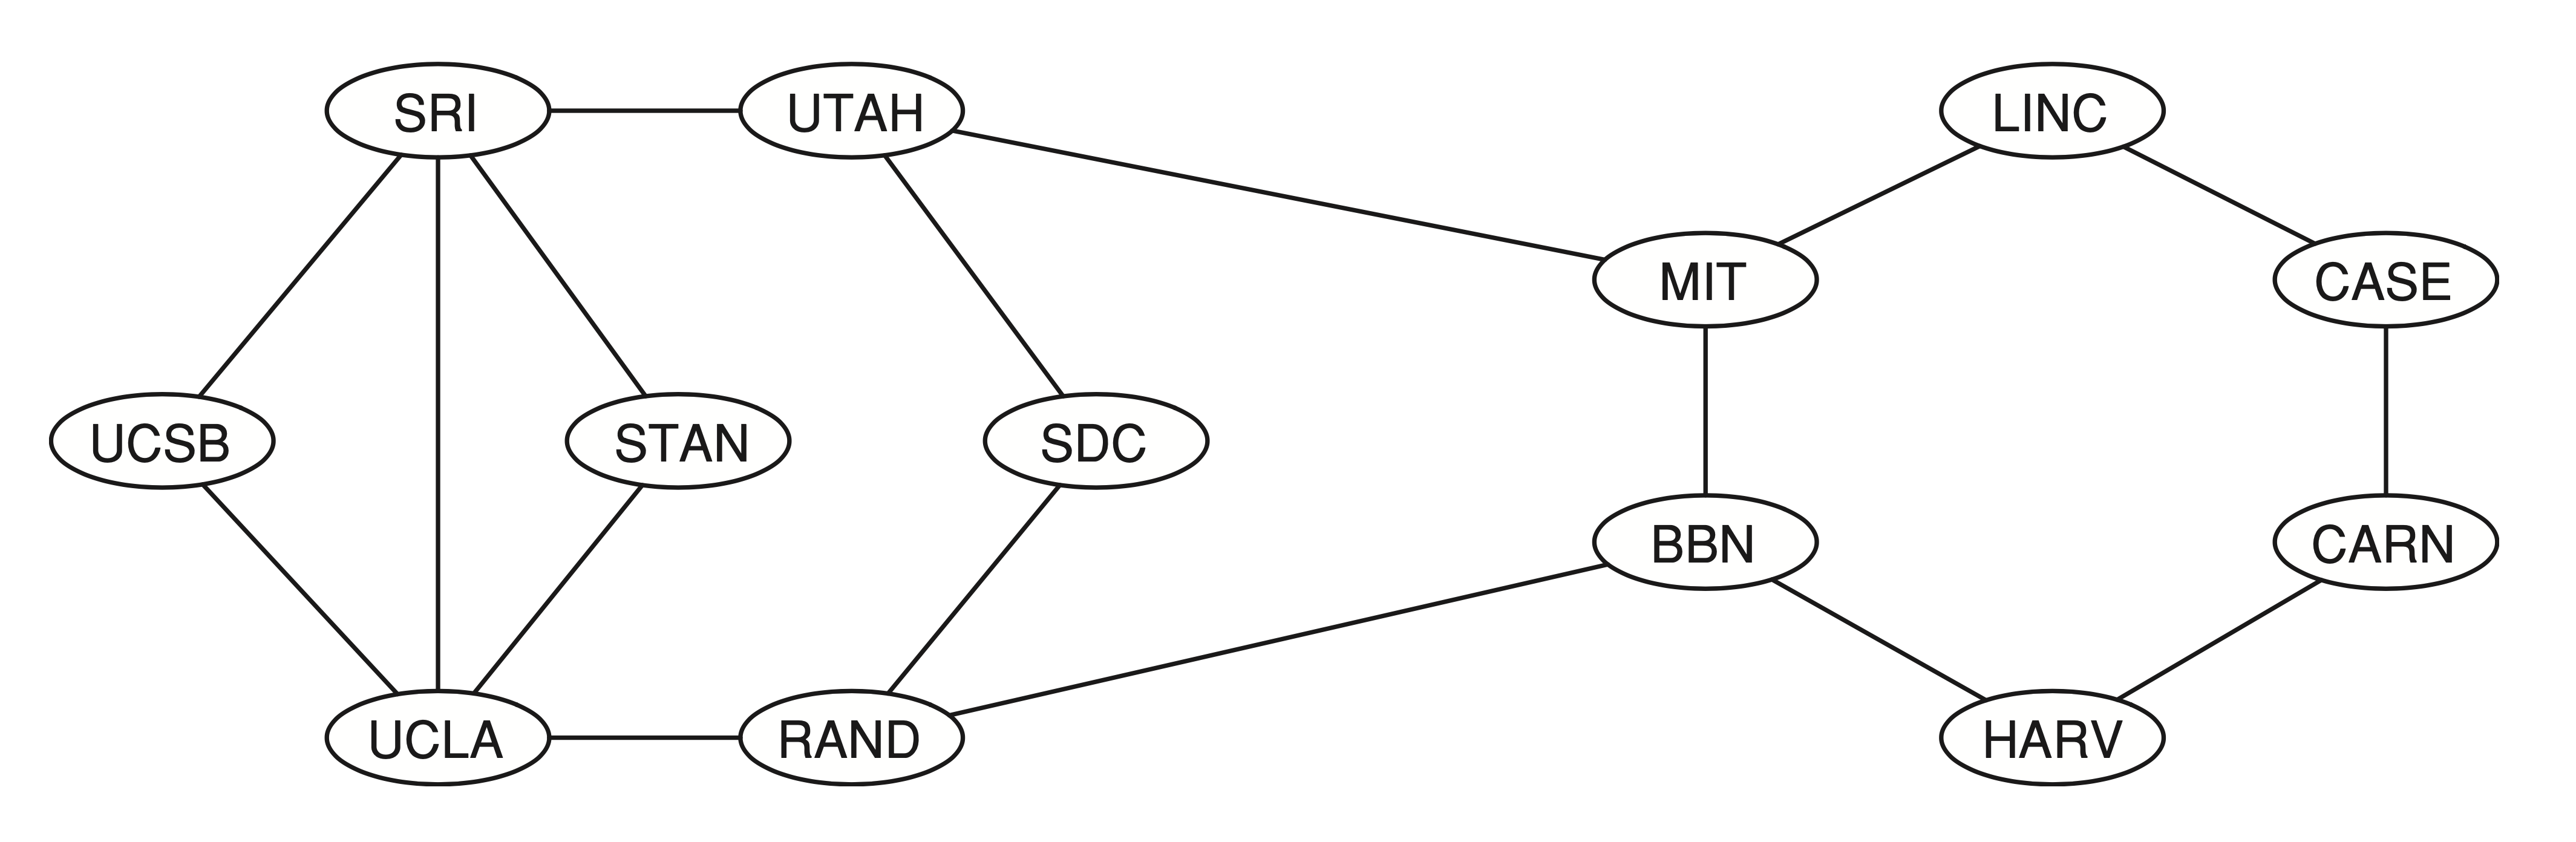
\includegraphics[scale=0.15]{Easley2010fig2_3.png}
			\caption{1970년 ARPANET}
			\label{fig:internetin1970}
			\end{center}
			\end{figure}
	\item 연결 (connected)
		\begin{itemize}
		\item 모든 노드 쌍에 경로가 있을 때 그래프가 연결되었다고 정의할 수 있음
		\item[예)] 그림 \ref{fig:internetin1970}
		\end{itemize}
	\item 컴포넌트 (component)
		\begin{itemize}
		\item 내부적으로 연결되어 있음
		\item 그래프의 다른 부분과 연결된 엣지가 없음
		\end{itemize}
	\item 경로의 길이 (length)
		\begin{itemize}
		\item 경로에 포함된 엣지의 수
		\item[예)] MIT -- BBN -- RAND -- UCLA $\rightarrow$ 3개
		\end{itemize}
	\item 두 노드의 거리 (distance)
		\begin{itemize}
		\item 두 노드의 가장 짧은 경로의 길이
		\item[예)] LINC -- SRI 의 거리: 3
		\item[활용)] 친구 -- 친구의 친구 -- 친구의 친구의 친구 -- $\cdots$
			\begin{itemize}
			\item ``작은 세계 현상 또는 분리의 여섯 단계(small-world phenomenon or six degrees of separation)"
			\end{itemize}
		\end{itemize}
	\end{itemize}		
\end{itemize}

\section{네트워크 효과}
\begin{itemize}
\item 네트워크가 경제 주체에 미치는 영향
	\begin{enumerate}
	\item 네트워크를 통해 정보를 전달
	\item 네트워크를 통해 이득을 전달 $\rightarrow$ 네트워크 효과
	\end{enumerate}
\item 네트워크 효과
	\begin{itemize}
	\item 어떤 재화나 서비스의 사용자 수가 늘어날 수록 그 가치가 더 높아짐\footnote{네트워크의 규모를 측정하면, 네트워크의 가치를 어림짐작할 수 있음. 네트워크의 규모를 측정하는 방법으로는 $n$개의 노드가 있을 때, 연결 방법에 따라 $n$ (사르노프의 법칙, Sarnoff's Law), $2^{n}$ (리드의 법칙, Reed's law), $n^{2}$ (멧칼프의 법칙, Metclafe's Law) 등으로 측정할 수 있다.}
	\end{itemize}	
\item $\rightarrow$ 네트워크의 양의 외부성
	\begin{itemize}
	\item 외부성
		\begin{itemize}
		\item 어떤 경제 행위가 제 3자에게 누출 편익(spillover benefit) 또는 누출 비용(spillover cost)을 주는 것
		\item 양의 외부성(또는 외부경제)
			\begin{itemize}
			\item 타인에게 누출 편익을 줄 때
			\item[예)] 어떤 집 주인이 집의 색을 바꾸고 정원을 꾸밈 $\rightarrow$ 이웃은 그로부터 즐거움을 느낄 수 있음 $\rightarrow$ 하지만 주인은 이웃의 그런 이득에 대해 이웃으로부터 대가를 받지 않음
			\end{itemize}
		\item 음의 외부성(또는 외부불경제)
			\begin{itemize}
			\item 타인에게 누출 비용을 부과할 때
			\item[예)] 운전자는 자신의 목적에 따라 차량을 운전 $\rightarrow$ 도로 용량을 넘는 차량이 몰리면 교통 체증이 시작 $\rightarrow$ 통행 시간의 증가(비용 발생), 하지만 각 운전자는 서로에게 비용을 지불하지 않음
			\end{itemize}
		\end{itemize}
	\item 네트워크의 양의 외부성
		\begin{itemize}
		\item 네트워크에 연결되어 있는 것의 가치가 네트워크의 크기와 함께 증가하기 때문		
		\item[예)] 다른 사람이 아래아 한글을 쓸 때는 아래아 한글을, MS 워드를 쓰고 있다면 MS 워드를 쓰는 것이 유리
		\end{itemize}
	\end{itemize}
\item 직접 대 간접
	\begin{itemize}
	\item 직접: 거리가 짧은 노드로 부터 얻는 효과
		\begin{itemize}
		\item 친구의 정보
		\end{itemize}
	\item 간접:  거리가 먼 노드로 부터 얻는 효과
		\begin{itemize}
		\item[예)] 게임 사용자 수의 증가 $\rightarrow$ 게임 개발사 유인, 운영 체제 사용자 증가 $\rightarrow$ 응용 프로그램 개발 유인
		\end{itemize}
	\end{itemize}
\item 네트워크에서 발생하는 양의 외부성은 양의 피드백을 가져옴	
	\begin{itemize}
	\item 양의 피드백
		\begin{itemize}
		\item 어떤 요인이 결과를 만들고, 이 결과가 다시 바로 그 요인을 더 강화시킴
		\item 양의 피드백이 있으면 강한 것은 더욱 강해지고, 약한 것은 더욱 약해짐
			\begin{itemize}
			\item 성장과는 다른 의미
			\item 양의 피드백은 하나의 방향으로 강화된다는 의미
			\item $\rightarrow$ 양의 피드백은 성장을 강화하기도 하지만 실패를 강화하기도 함
			\end{itemize}
		\end{itemize}
	\end{itemize}
\end{itemize}

\section{네트워크 효과의 경제적 의미}
\begin{itemize}
\item 수요에서 규모의 경제(Economies of Scale)
	\begin{itemize}
	\item 보통은 공급에서 규모의 경제: 생산량 증가함에 따라 평균 생산 비용 감소
	\item 수요에서 규모의 경제: 사용자 수의 증가에 따라 소비자가 부담할 비용의 감소
	\item[예)] 수강생이 많을 수록, 문제 해결을 위해 물어볼 수 있는 사람이 많아짐 $\rightarrow$ 질문/탐색의 비용이 낮아짐
	\end{itemize}
\item 소비자의 지불가능의사
	\begin{itemize}
	\item 재화나 서비스로부터 얻을 것으로 기대하는 효용에 따라 변화
	\item 네트워크 효과 $\rightarrow$ 소비자의 기대 효용을 높임 $\rightarrow$ 지불가능의사를 높임
		\begin{itemize}
		\item 어떤 소비자 $x$의 지불가능의사 $WTP_{x}$
		\item 어떤 재화나 서비스의 사용자 수가 $z$이고, 이로 인해 소비자가 얻는 이득을 $f(z)$라 하면
			\begin{itemize}
			\item 단, $0<z<1$ 이고, $f(\cdot)$는 $z$에 대해 증가 함수
			\item 즉, $z$가 증가함에 따라 그 값이 커지는 함수
			\end{itemize}
		\item 네트워크 효과가 있을 때의 지불가능의사는 $f(z)WTP_{x}$
		\end{itemize}
	\item 이 재화나 서비스의 가격이 $p$라면
		\begin{itemize}
		\item 소비자 $x$는 $f(z)WTP_{x} \geq p$ 일 때만 소비
		\end{itemize}
	\item 즉, 소비자 $x$가 예상하는 다른 소비자의 수 $z$ 가 중요
		\begin{itemize}
		\item 예상하는 다른 소비자 $z = 0$ 이라면 $\rightarrow$ 소비하지 않을 것
		\item 예상하는 소비자의 수가 충분하지 않다면 ($0< z < z^{'}$)
			\begin{itemize}
			\item $\rightarrow$ 다른 소비자도 그런 예상을 하고 있다면, 이 재화나 서비스에 대한 수요가 계속 감소 
			\item $\rightarrow$ 지불가능의사는 0으로 수렴
			\end{itemize}
		\item 예상하는 소비자의 수가 충분하다면 ($ z^{'} < z <  z^{''}$)
			\begin{itemize}
			\item $\rightarrow$ 다른 소비자도 그런 예상을 하고 있다면, 소비자 수가 계속 증가
			\end{itemize}
		\item 예상하는 소비자의 수가 너무 많다면 ($z^{''} < z < 1$)
			\begin{itemize}
			\item $\rightarrow$ 지불가능의사에 비해 가격이 너무 높으므로 소비가 감소 
			\item $\rightarrow$ 하지만 예상 소비자의 수가 많은 수준 근처에서 머물 것
			\end{itemize}
		\end{itemize}
	\end{itemize}
	
	\begin{figure}[htbp]
	\begin{center}
	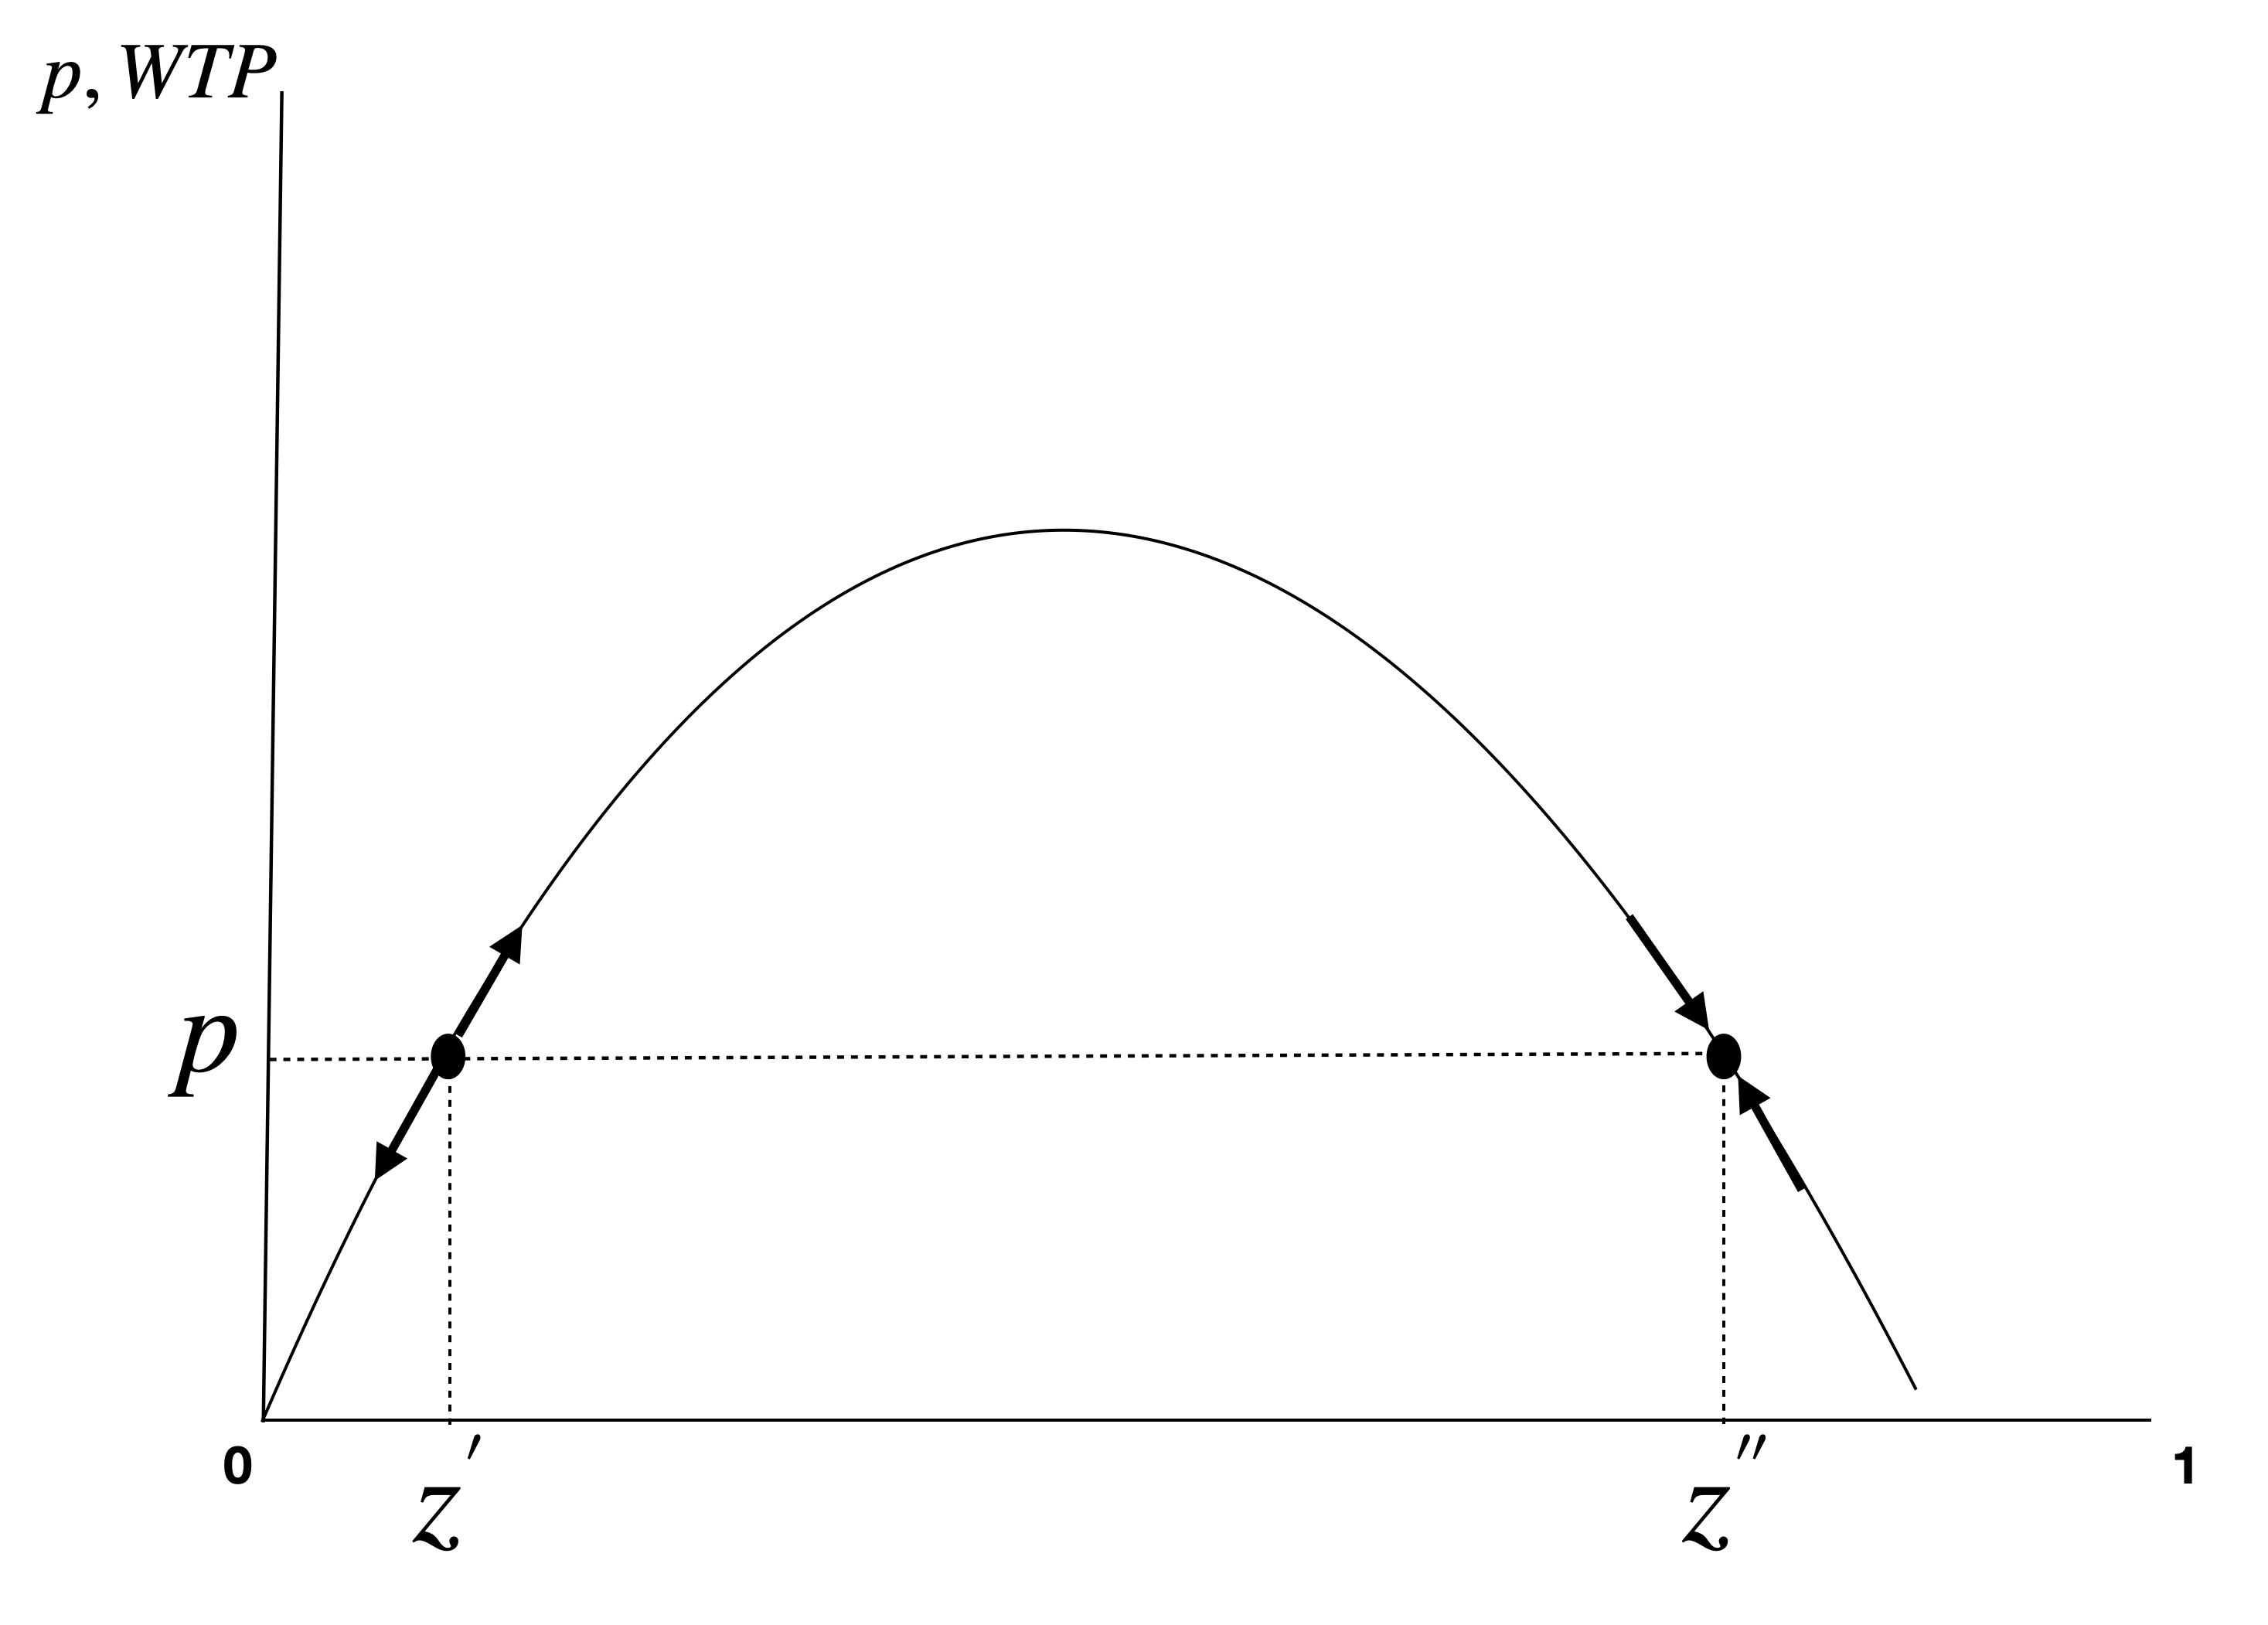
\includegraphics[scale=0.2]{criticalmass.png}
	\caption{네트워크 효과가 있는 시장에서의 균형}
	\label{fig:criticalmass}
	\end{center}
	\end{figure}

	
	
\item 임계 질량(critical mass)
	\begin{itemize}
	\item 우리는 스스로 지속 가능한(self-sustaining) 규모로 정의: ``알아서 잘 굴러가는"  $\rightarrow$ 양면 모두에서 필요할 수 있음
		\begin{itemize}
		\item 임계 질량은 원래 핵분열성 물질이 연쇄 반응을 일으킬 수 있는 최소의 질량을 의미 
		\item 핵분열성 물질의 핵에 중성자가 충돌하면 핵분열이 일어남 $\rightarrow$ 다시 중성자를 방출 $\rightarrow$ 이 중성자가 다시 근처의 핵에 충돌 $\rightarrow$ 연쇄 반응 
		\item 만약 충분한 야의 핵분열성 물질이 있지 않다면, 방출된 중성자가 근처의 핵에 충돌하지 않고 연쇄 반응이 일어나지 않을 수 있음. 플루토늄 239의 임계 질량은 약 11kg(24.2파운드)
		\end{itemize}
	\end{itemize}	
\item $\rightarrow$ 사용자 수의 초기 확보와 유지가 중요: \ref{cha:ecommerce}--\ref{cha:chikenandeggproblem} 장의 주제
	\begin{itemize}
	\item 지금까지의 논의만 생각해보면
		\begin{itemize}
		\item $p$가 낮은 수준이면, 즉 가격을 낮추면,
		\item $z^{'}$를 낮은 수준으로 $z^{''}$를 높은 수준으로 유지할 수 있음
		\item $\rightarrow$ 하지만, 기업은 손실을 입을 수 있음
		\item $\rightarrow$ 그러나, 시소 원칙과 같이 생각해볼 것
		\item $\rightarrow$ 또, 사용자 수의 증가로 인해 사업 영역의 확대도 가능
		\end{itemize}
	\item 페이스북(Facebook)
		\begin{itemize}
		\item 하버드 대학교와 그외 아이비리그 대학생의 회원 가입
		\item $\rightarrow$ 회원 대상의 증가
		\item $\rightarrow$ 게임(Farmville)과 어플리케이션
		\item $\rightarrow$ 타겟 광고
		\end{itemize}
	\item 에어비앤비(Airbnb) 등 다른 기업 사례
		\begin{itemize}
		\item \url{https://www.slideshare.net/a16z/network-effects-59206938} (영문)
		\end{itemize}	
	\end{itemize}
\item 네트워크 효과가 강한 산업
	\begin{itemize}
	\item 높은 진입 장벽으로 작동 
	\end{itemize}
\end{itemize}

\pagebreak

\section*{정리하기}
\begin{enumerate}
\item 네트워크는 노드와 링크로 연결되어 있는 구조이고, 주로 양의 외부성을 일으킨다. 
\item 네트워크에서 양의 외부성은 양의 피드백을 가져온다.
\item 양의 외부성은 어떤 경제 행위가 제3자에게 누출 편익을 주는 것이다.
\item 양의 피드백은 어떤 요인이 결과를 만들고 이 결과가 다시 그 요인을 더 강화시키는 것으로, 양의 피드백이 있으면, 어느 하나의 방향이 강화되는 효과가 나타난다.
\item 네트워크 효과는 소비자의 지불가능의사를 높이고, 소비자의 지불 가능의사가 소비자의 수에 따라 역 U자의 형태를 갖는다고 할 때, 예상하는 전체 소비자의 수가 적은 상태는 기대 효용이 주어진 가격보다 낮아지게 되어 결국 소비를 하지않게 된다. 그리고 양의 피드백으로 이 방향은 더욱 강화된다. 따라서 적은 수의 소비자는 안정적인 균형이 아니다.
\item 하지만, 예상하는 전체 소비자의 수가 많은 상태에서는 그 소비자 수가 더 늘어 소비기대 효용이 주어진 가격보다 낮아지더라도, 결국 많은 수준의 예상 소비자 수준으로 복귀한다. 따라서 많은 수의 소비자는 안정적인 균형이다.
\item 이는 네트워크 효과가 있는 시장에서 일정 수의 소비자 수를 확보하면 안정적으로 사업을 운영할 수 있음을 의미하고 이를 임계 질량이라고 할 수 있다.
\item 따라서 네트워크 효과가 있는 시장에서는 사용자 수의 초기 확보와 유지가 중요하다. 가장 간단한 전략은 가격을 낮춰 안정적인 소비자 수가 될 수 있는 수준을 낮추는 것이다.
\item 가격을 낮추더라도 양면 시장에서의 시소 원칙을 사용하면 플랫폼은 손해를 보지 않을 수 있고, 다른 한편 사용자 수를 늘리게 되면 다른 사업으로의 확장이 가능해진다.
\item 그러나 사용자 수를 초기에 확보하는 것이 쉬운 일은 아니므로 네트워크 효과가 강한 시장에 신규 기업이 진입하기 어려운 진입 장벽이 될 수 있다.
\end{enumerate}
%\chapter*{보론: 네트워크의 규모 측정 방법} \addcontentsline{toc}{chapter}{보론: 네트워크의 규모 측정 방법}  
\section*{네트워크의 규모 측정} \addcontentsline{toc}{section}{네트워크의 규모 측정}  
%\subsection*{20세기 이전 경제사학} \addcontentsline{toc}{subsection}{20세기 이전 경제사학}  
\begin{itemize}
\item 멧칼프의 법칙
\end{itemize}
\chapter{데이터 기반 의사 결정}\label{cha:databaseddecision}

\section*{학습개요}
 플랫폼 산업의 디지털화가 가져온 특징과, 경제학의 관점에서 기계 학습 또는 빅데이터 분석에 기반한 의사 결정이 어떤 의미가 있는 지 살펴본다.


\section*{학습목표}
\begin{enumerate}
\item 디지털 플랫폼의 특징을 설명할 수 있다.
\item 데이터 기반 의사 결정의 절차를 설명할 수 있다.
\item 데이터 기반 의사 결정으로 좋은 결과를 얻을 수 있는 조건을 설명할 수 있다.
\item 빅 데이터와 기계학습이 의사 결정에 미친 영향을 비용 하락으로 설명할 수 있다.
\item 데이터 활용 또는 빅데이터 분석이 경제의 어떤 비용을 낮추는 지 설명할 수 있다.
\end{enumerate}

\section*{주요 용어}
기계학습, 산업 간 데이터 마이닝 표준 절차, 예측, 의사결정, 정보의 디지털 화, 디지털 경제의 비용 하락

\pagebreak

\section{디지털 플랫폼과 데이터}
\begin{itemize}
\item 전통적인 플랫폼 산업의 변화
	\begin{itemize}
	\item 광고 산업
		\begin{itemize}
		\item 전통적으로 광고 효과를 높일 수 있는 콘텐츠(attention attractors)와
		\item 광고의 효과를 파악/예측할 수 있는 중개 수단(attention brokerage)이 필요
		\end{itemize}
	\item 디지털화 $\rightarrow$ 중개 수단의 광고 효과 파악/예측의 정확도가 올라감
	\end{itemize}
\item 디지털 플랫폼
	\begin{itemize}
	\item 과거의 플랫폼에 비해
		\begin{itemize}
		\item 사용자의 데이터를 더 많이 더 폭 넓게 수집, 유지, 활용
		\item 관련된 부가 서비스의 개발
		\end{itemize}
	\end{itemize}	
\item 뉴스 애그리게이터(News aggregator)
	\begin{itemize}
	\item 알고리듬을 이용, 뉴스를 자동으로 모아서 전달
	\item 어떤 기준으로 모을 것인가? $\rightarrow$ 독자의 취향에 따라야 함
		\begin{itemize}
		\item 이전의 뉴스 검색 기록을 토대로 추천 $\rightarrow$ 독자가 선호하는 콘텐츠를 검색할 시간을 줄여줌
		\end{itemize}
	\item 다양한 파생 문제 %$\rightarrow$ \ref{cha:newsandadvertisement}장
		\begin{itemize}
		\item 균형 잡힌 시각이 아니라, 독자의 선호에 맞는 편향된 시각의 뉴스만 제공
		\item 가십성 또는 감동적인 이야기 위주의 제공
		\item 저작권 침해 여부 및 이와 관련된 경제적 보상 문제
		\end{itemize}
	\end{itemize}
\end{itemize}

\section{데이터 기반 의사 결정}\label{sec:databaseddecision}
\subsection{데이터 기반 의사 결정}
\begin{itemize}
\item 의사 결정(decision making)
	\begin{itemize}
	\item 주어진 조건에서 어떤 행동의 실행 여부를 결정
	\item 차도의 신호등이 붉은 색, 인도의 신호등이 파란색 $\rightarrow$ 차를 멈추어야 함
	\end{itemize}
\item 경제 주체는 의사 결정에 항상 직면
	\begin{itemize}
	\item 기업: 주어진 재고 현황에서 제품 A의 생산을 늘려야할 지 줄여야할 지 등
	\item 중앙은행: 현재 경제 상황에서 이자율을 높여야할 지 낮추어야할 지 등
	\end{itemize}	
\item 데이터는 어디에나 있음
	\begin{itemize}
	\item 기업 내: 기업 운영, 공급 사슬, 작업 절차, 소비자 행동, 마케팅 성과 등
	\item 기업 외: 경쟁자 동향, 산업 동향, 거시 경제 상황 등
	\end{itemize}
\item 데이터 기반 의사 결정
	\begin{itemize}
	\item 주어진 조건 $\rightarrow$ 데이터 화 $\rightarrow$ 의사결정
	\end{itemize}	
\item 데이터 분석과 경제학
	\begin{itemize}
	\item 기계 학습 또는 빅데이터 분석의 최종 단계 $\rightarrow$ 결과를 어떻게 유용하게 사용할 것인지 생각해야 함
	\item 경제학은 제약 조건에서의 최적화라는 시각을 통해, 유용한 의사 결정의 방향을 제시
	\end{itemize}
\end{itemize}

\subsection{데이터 분석의 목적과 절차}
\begin{itemize}
\item 데이터 기반 의사 결정의 순서
	\begin{enumerate}
	\item 데이터 수집 및 가공
		\begin{itemize}
		\item 도로 이미지, 라이다 정보, 레이더 정보 등
		\item $\rightarrow$ 기계가 처리 가능한 형태로 전환
		\end{itemize}
	\item 기계 학습 (machine learning)
		\begin{itemize}
		\item 데이터를 분석하는 수학적 절차 (알고리듬)
		\item 주어진 사진 $\rightarrow$ 신호등과 현재 교통 신호를 학습
		\end{itemize}
	\item 데이터 분석
		\begin{itemize}
		\item 목적: 데이터가 표상하는 것 간의 유용한 패턴 또는 상관 관계를 찾는 것
		\item 차도의 신호등이 붉은색, 인도의 신호등이 파란색
			\begin{itemize}
			\item $\rightarrow$ 차는 멈추고 사람은 인도를 건너감
			\end{itemize}
		\end{itemize}
	\item 패턴 또는 상관 관계 파악
		\begin{itemize}
		\item 데이터가 표상하는 것의 새로운 사례에 대한 추론 (inference)
		\item 새로운 도로에서 무엇이 신호등이고, 신호는 무슨 색인가?
		\end{itemize}
	\item 의사결정
		\begin{itemize}
		\item 새로운 거리에서 차도의 신호등이 붉은 색, 인도의 신호등이 파란색
		\item  $\rightarrow$ 차를 멈추어야 함
		\end{itemize}	
	\end{enumerate}
\item 산업 간 데이터 마이닝 표준 절차(CRISP-DM: Cross-Industry Standard Process for Data Mining)
	\begin{enumerate}
	\item 사업에 대한 이해
		\begin{itemize}
		\item 가장 먼저, 그리고 가장 중요한 것은 올바른 질문을 하는 것 또는 문제를 정확히 찾는 것
		\item 창의적이고 개방적인 자세로 문제 해결을 위한 가설을 수립
		\end{itemize}
	\item 데이터에 대한 이해
		\begin{itemize}
		\item 가공할 수 있는 데이터를 정확히 이해해야 함
		\item 이전 단계에서 생각한 문제점 또는 해결 가설을 검토할 수 있는 데이터를 다각도로 확인해야 함
		\end{itemize}
	\item 데이터 가공
		\begin{itemize}
		\item 가장 많은 시간이 들어가는 작업이 될 수 있음
		\item 데이터와 사업 분야에 대한 이해가 충분한 인력으로 팀을 구성하는 것이 바람직
		\item 데이터 가공 기술이 있는 인력과 사업 운영 능력이 있는 인력이 한 팀이 되는 것을 검토
		\end{itemize}
	\item 모형화 
		\begin{itemize}
		\item 사용 가능한 데이터로 해결 가설을 지지할 수 있는 지, 다양한 알고리듬으로 분석
		\item 좋은 착안점을 줄 수 있을 때까지 인내심을 갖고 데이터를 계속 다룰 수 있어야 함
		\end{itemize}
	\item 모형 평가
		\begin{itemize}
		\item 첫번째 결과를 그대로 받아들이면 안됨
		\item 다양한 기법, 시나리오 분석 등을 통해, 결과에 대한 신뢰성을 높여야 함
		\end{itemize}
	\item 결과 활용
		\begin{itemize}
		\item 충분한 수준의 신뢰성을 확보했다면, 사업 또는 기업 운영에 데이터 분석 결과를 활용해야 함
		\end{itemize}
	\end{enumerate}	
\item 정확한 문제 진단 $+$ 정확한 가설 $+$ 정확한 데이터 $\rightarrow$ 좋은 결과
\item 연관 규칙 학습(association rule learning)
	\begin{itemize}
	\item 어떤 상품 또는 서비스를 다른 상품 또는 서비스와 묶어 파는 것이 유리한가? 
		\begin{itemize}
		\item $\rightarrow$ 교차 마케팅, 교차 판매, 카탈로그  설계, 쇼핑몰 사이트 디자인, 온라인 광고 최적화, 가격 결정, 프로모션 설계 등에 활용
		\end{itemize}
	\item 정의 및 유용한 개념
		\begin{itemize}
		\item 아이템 $I=\{i_{1}, i_{2}, \ldots, i_{n} \}$		
		\item 거래 데이터 베이스 $D = \{t_{1}, t_{2}, \ldots, t_{n} \}$
		\item 관계 규칙(association rule) $X \Rightarrow Y$, 단 $X,Y \subseteq I$
		\item 지지도(support) $supp(X) = \dfrac{|t \in T; X \subseteq t|}{|T|}$
		\item 신뢰도(confidence) $ conf(X \Rightarrow Y) = \dfrac{supp(X \cup Y)}{supp(X)} $
			\begin{itemize}
			\item $supp(X \cup Y) \rightarrow P(E_{X} \cap E_{Y})$
			\item $conf(X \Rightarrow Y) \rightarrow P(E_{Y}|E_{X}) $
			\end{itemize}
		\end{itemize}	
	\item 모두 1,000번의 거래 기록이 있고, 이 중 $X$가 팔린 기록은 300번, $X$와 $Y$가 같이 팔린 기록은 150번
		\begin{itemize}
		\item $supp(X) = \dfrac{150}{1000} = 15\%$
		\item $conf(X \Rightarrow Y) = \dfrac{150}{300} = 50\%$ 
		\end{itemize}		
	\end{itemize}	
\item 연관 규칙 학습의 예
	\begin{itemize}
	\item 판매 기록
		\begin{table}[htp]
		\caption{판매 기록의 예}
		\begin{center}
		\begin{tabular}{lllll}
		\toprule
		구매자	 & 구입품 1 & 2  & 3  & 4 \\
			\midrule
		 1 & 우유 & 계란 & 빵 & 딸기잼 \\
		 2 & 우유 & 딸기잼 & 계란 & 포도잼 \\
		 3 & 빵 & 딸기잼 & 포도잼 & \\
		 4 & 우유 & 빵 & 딸기잼 & \\
		 5 & 빵 & 딸기잼 & 소시지 & \\
		 6 & 우유 & 빵 & 딸기잼 & 소시지 \\
		 7 & 우유 & 소시지 & & \\
		 8 & 우유 & 빵 & 딸기잼 & \\
		 9 & 빵 & 딸기잼 & 계란 & 소시지 \\
		 10 & 우유 & 딸기잼 & 빵 & \\
		 11 & 우유 & 빵 & 딸기잼 & \\
		 12 & 우유 & 빵 & 소시지 & 포도잼 \\
		\bottomrule
		\end{tabular}
		\end{center}
		\label{tab:transactionlist}
		\end{table}%
	\item 주어진 데이터에서는 모든 발생 사건의 확률을 구할 수 있으므로 관심있는 사건으로 좁힘 $\rightarrow$ 관심있는 사건의 기준을 설정해야 함
		\begin{itemize}
		\item 어떤 제품 집합이 자주 팔림: $supp(X) \geq 33\%$
		\item 어떤 제품 집합 $X$가 판매되었을 때, 다른 제품 집합 $Y$가 팔릴 확률: $conf(X \rightarrow Y) \geq 50\%$
		\end{itemize}
	
\pagebreak	
		
	\item 판매 기록의 축약
		\begin{enumerate}
		\item 각 제품($x_{i}$)의 판매 횟수를 계산
			\begin{table}[htp]
%			\caption{default}
			\begin{center}
			\begin{tabular}{ll}
			\toprule
%			 & \\
%			\midrule
			우유& 9 \\
			빵 & 10 \\
			딸기잼 & 10 \\
			계란 & 3 \\
			포도잼 & 3 \\
			소시지 & 5 \\
			\bottomrule
			\end{tabular}
			\end{center}
			\label{tab:allitems}
			\end{table}%
		\item 자주 팔리는 제품($supp(x_{i}) \geq 33\%$)만  추출		
			\begin{table}[htp]
%			\caption{default}
			\begin{center}
			\begin{tabular}{ll}
			\toprule
%			 & \\
%			\midrule
			우유& 9 \\
			빵 & 10 \\
			딸기잼 & 10 \\
			소시지 & 5 \\
			\bottomrule
			\end{tabular}
			\end{center}
			\label{tab:featureditems}
			\end{table}%		
		\item 두 제품이 같이 팔린 경우를 추출 
			\begin{itemize}
			\item $\rightarrow$ 자주 팔리는 조합 4개: (우유, 빵), (우유, 딸기쨈), (빵, 딸기잼), (빵, 소시지)
			\end{itemize}	
				\begin{table}[htp]
	%			\caption{default}
				\begin{center}
				\begin{tabular}{ll}
				\toprule
	%			 & \\
	%			\midrule
				우유, 빵 & 7 \\
				우유, 딸기쨈 & 7 \\
				우유, 소시지 & 3 \\
				빵, 딸기잼 & 9 \\
				빵, 소시지 & 4 \\
				딸기잼, 소시지 & 3\\
				\bottomrule
				\end{tabular}
				\end{center}
				\label{tab:twoitemssets}
				\end{table}%			
		\item 세 제품이 팔린 경우를 추출
			\begin{itemize}
			\item $\rightarrow$ 자주 팔리는 조합 1개: (우유, 빵, 딸기쨈)		
				\begin{table}[h!]
	%			\caption{default}
				\begin{center}
				\begin{tabular}{ll}
				\toprule
	%			 & \\
	%			\midrule
				우유, 빵, 딸기쨈 & 6 \\
				우유, 빵, 소시지 & 1 \\
				빵, 딸기잼, 소시지 & 3 \\
				\bottomrule
				\end{tabular}
				\end{center}
				\label{tab:threeitemssets}
				\end{table}%		
			\end{itemize}									
		\item 소비 예측 $\rightarrow$ 모두 기준을 통과			
			\begin{enumerate}
			\item (빵, 딸기잼) $\rightarrow$ 우유
				\begin{itemize}
				\item $supp(A) = \dfrac{6}{12} = 50\%$
				\item $conf(A \Rightarrow B) = \dfrac{6}{9} = 67\%$
				\end{itemize}
			\item (우유, 빵) $\rightarrow$ 딸기잼
				\begin{itemize}
				\item $supp(C) = \dfrac{6}{12} = 50\%$
				\item $conf(C \Rightarrow D) = \dfrac{6}{7} = 86\%$
				\end{itemize}
			\item (우유, 딸기잼) $\rightarrow$ 빵
				\begin{itemize}
				\item $supp(E) = \dfrac{6}{12} = 50\%$
				\item $conf(E \Rightarrow F) = \dfrac{6}{7} = 86\%$
				\end{itemize}
			\end{enumerate}				
		\end{enumerate}	
	\item 상품 두 개의 조합을 검토할 수도 있음
		\begin{itemize}
		\item 많은 상품 조합이 가능 $\rightarrow$ 관심이 있는 조합을 먼저 정해야 함을 의미
		\end{itemize}
	\end{itemize}
\item $\rightarrow$ 구매 가능성 높은 상품의 추천, 재고 및 생산 관리 등
\item 주의할 점
	\begin{itemize}
	\item (우유, 딸기잼, 빵)을 묶어서 팔 때, 판매 가능성이 높다는 결론에 도달?
	\item 다른 요소를 고려해야 함
		\begin{itemize}
		\item 묶음 가격은 검토하지 않음 $\rightarrow$ 지불가능의사 파악 필요 
		\item 또한, 모든 조합이 사업에 의미가 있는 것은 아님 $\rightarrow$ 묶음의 비용 등도 고려해야 함
		\end{itemize}
	\end{itemize}
\end{itemize}

\section{예측의 경제적 효과}
\begin{itemize}
\item 예측
	\begin{itemize}
	\item 데이터 분석의 결과를 예측에 활용
	\item 빅데이터와 기계 학습 $\rightarrow$ 예측 비용의 하락
	\end{itemize}
\item 예측 $+$ 평가 $\rightarrow$ 의사결정
	\begin{itemize}
	\item 예측과 의사결정이 동일하지 않음
		\begin{itemize}
		\item 오후에 비가 내릴 확률이 80\%이면 아침에 우산을 갖고 출근
		\item 오후 7시에 비가 내릴 확률이 50\%이고, 오후 8시에 비가 내릴 확률이 80\%라면, 퇴근 시간에 따라 우산을 준비할 지 결정
		\item 하지만, 비를 맞는 것이 부담스럽지 않은 사람이면, 크게 신경쓰지 않고 우산을 준비하지 않을 것
		\end{itemize}	
	\item 평가 $\rightarrow$ 인간의 역할
	\end{itemize}	
\item 기계적 의사 결정과 도덕률
	\begin{itemize}
	\item 인간의 평가가 없는 의사 결정 $\rightarrow$ 기계적 규칙이 필요
	\item 소시지 소비자 분석 결과
		\begin{itemize}
		\item 맥주를 살 확률 $>$ 90\% 소비자 $\rightarrow$ 마케팅 필요 없음
		\item 1\% $\leq$ 맥주를 살 확률 $\leq$ 90\% $\rightarrow$ 할인 쿠폰 발송
		\item  맥주를 살 확률 $\leq$ 1\% $\rightarrow$ 마케팅 필요 없음
		\end{itemize}
	\item 충분?
		\begin{itemize}
		\item 미성년자에게 마케팅하면 안됨
		\item 기록이 있다면, 알코올 의존이 강한 소비자에게 마케팅하면 안 됨
		\end{itemize}
	\item $\rightarrow$ 기계적 규칙을 사회적 규범에 맞출 필요가 있음
	\end{itemize}	
\item 예측 비용 하락의 경제적 효과
	\begin{itemize}
	\item 예측을 중간재로서 사용하는 수요 증가
		\begin{itemize}
		\item 예
			\begin{itemize}
			\item 도로 상황을 파악 $\rightarrow$ 운전
			\item 자율 주행: 사람 운전자가 어떻게 하는 가를 예측하는 문제로 전환
			\end{itemize}
		\item $\rightarrow$ 보완재의 가치를 높임
			\begin{itemize}
			\item 데이터 수요 증가
			\item 평가(judgement)가 부가가치를 창출
			\end{itemize}
		\item $\rightarrow$ 대체되는 것의 가치를 낮출 것	
		\end{itemize}
	\item 불확실성 감소
		\begin{itemize}
		\item 기계학습은 어떤 결과가 나타날지의 가능성을 제시
		\item 어떤 구매자의 구매 기록에 쌀, 맥주, 닭강정이 있다고 가정
			\begin{itemize}
			\item 기계학습을 통해, 다음 구매에 
			\item 쌀을 살 확률 80\%, 맥주를 살 확률 15\%, 닭강정을 살 확률 5\%로 추정
			\end{itemize}
		\item $\rightarrow$ 불확실성을 낮춤
		\end{itemize}	
	\end{itemize}
\item 예측 방법
	\begin{itemize}
	\item 확률: 분류 모형(classification model)을 주로 사용
		\begin{itemize}
		\item (어떤 조건의) 소비자가 쌀을 살 확률
		\item $\rightarrow$ 질병 진단, 콘텐츠 분류, 소비자 이탈, 사기 감지, 상품 추천, 기계 고장 등
		\end{itemize}
	\item 규모: 회귀 모형(regression model)을 주로 사용
		\begin{itemize}
		\item 소비자가 한 번의 구매에서 사는 쌀의 양
		\item $\rightarrow$ 기대 수명, 이동 시간, 대출 손실, 소비 규모, 구매 간격, 통화 시간, 반응 시간 등
		\end{itemize}
	\end{itemize}	
\end{itemize}

\pagebreak

\section*{정리하기}
\begin{enumerate}
\item 디지털 플랫폼은 과거의 플랫폼에 비해 사용자의 데이터를 더 많이 더 폭 넓게 수집, 유지, 활용하고, 이를 바탕으로 관련된 부가 서비스를 개발할 수 있다는 특징이자 장점을 갖고 있다.
\item 정확한 문제 진단, 정확한 가설, 정확한 데이터가 결합될 때 좋은 결과를 얻을 수 있다.
\item 연관 규칙 학습은 지지도와 신뢰도를 기준으로, 어떤 상품 또는 서비스와 다른 상품 또는 서비스의 소비 관계를 설명한다.
\item 빅데이터의 기계 학습으로 예측 비용이 하락했다. 
\item 예측에 평가를 결합하여 의사 결정을 내린다.
\item 예측 비용이 하락하므로 예측을 중간재로 사용하는 수요가 늘어나고, 따라서 예측을 보완하는 상품이나 서비스의 가치는 높아지지만, 대체되는 상품이나 서비스의 가치는 낮아진다.
\item 데이터의 활용 또는 빅데이터 분석은 탐색, 추적, 인증 비용을 낮춘다.
\end{enumerate}
\chapter{시장 설계}\label{cha:mechanismdesign}

\section*{학습개요}
게임 이론과 경매 이론의 기본 모형을 학습한다. 그리고 이를 검색어 경매에 활용할 수 있음을 배운다.

\section*{학습목표}
\begin{enumerate}
\item 게임 이론의 기본 모형을 이해한다.
\item 경매 이론의 기본 모형을 이해한다.
\item 제2가격 입찰제의 기본 모형을 이해한다.
\item 제2가격 입찰제가 검색어 경매에 활용될 수 있음을 이해한다.
\item 전략적 행위자가 자신의 이익을 위해 행동하더라도 사회적으로 바람직한 목적을 달성하도록 보장할 수 있는 제도를 만들 수 있음을 이해한다.
\end{enumerate}

\section*{주요 용어}
상호의존성, 전략적 행동, 균형, 시장 설계, 제2가격 입찰제

\pagebreak

\section{게임 이론}
\begin{itemize}
\item 게임 이론
	\begin{itemize}
	\item 다수의 경제 주체 간에 상호 의존성이 있어 전략적 고려를 할 때의 합리적인 의사 결정을 연구
		\begin{itemize}
		\item 상호 의존성
			\begin{itemize}
			\item 자신의 의사결정이 자신의 효용뿐만 아니라 다른 경제주체의 효용에도 영향을 미침
			\item 동시에 다른 경제주체의 의사결정도 자신의 효용에 영향을 미침
			\end{itemize}
		\item 전략적 고려
			\begin{itemize}
			\item 경제주체가 상호의존성을 인식하고 자신에게 가장 유리한 의사결정을 하고자할 때
			\item 다른 경제주체의 의사결정이 자신의 효용에 미치는 영향을 고려
			\end{itemize}
		\end{itemize}
	\item 상품을 걸고 하는 여러 사람의 가위바위보
		\begin{itemize}
		\item 내가 가위를 내더라도, 상대방이 가위, 바위, 보 중 무엇을 내느냐에 따라 내가 이기고 지는 것이 달라짐 $\rightarrow$ 승패에 따라 얻는 것이 달라짐
		\item 내가 이기려면 상대가 무엇을 낼 지 생각해야 함 
		\item 상대도 마찬가지 
		\end{itemize}
	\item 기업의 신상품 출시, 생산량 결정 등 경쟁 전략, 투자, 투표 등도 같은 구조로 생각할 수 있음
	\end{itemize}
\item 게임의 표현
	\begin{itemize}
	\item 경기자(player): 게임 참여자, $n$명의 경기자가 참여할 경우
		\begin{align*}
		I = \{1, 2, \cdots, n \}
		\end{align*}
	\item 전략 (strategy): 경기자가 선택할 수 있는 대안 $s_{i}$
		\begin{itemize}
		\item 전략 집합: 경기자가 선택할 수 있는 전략의 집합 $s_{i} \in S_{i}$
		\item 전략 프로필: 각 경기자가 자신의 전략 집합에서 전략을 선택하여 나열한 것 $(s_{1}, s_{2})$
		\end{itemize}
	\item 보수함수 (payoff function): 가능한 모든 전략 프로필에 대해 경기자가 얻는 보상 $u_{i}$
	\item 2 명의 가위바위보
				\begin{table}[htp]
				\caption{2명의 가위바위보 게임}
				\begin{center}
				\begin{tabular}{cccc}
				\toprule
				 & 가위 & 바위 & 보\\
				\midrule
				 가위 & 0 ,0 & -1, 1 & 1, -1 \\
				 바위 & 1, -1 & 0, 0 & -1, 1 \\
				 보 & -1, 1 & 1, -1 & 0 ,0 \\
				\bottomrule
				\end{tabular}
				\end{center}
				\label{tab:twopersonsrockpaperscissorsgame}
				\end{table}%
	\end{itemize}
\item 기본 가정
	\begin{itemize}
	\item 게임의 공통 지식(Common Knowledge of Games)
		\begin{itemize}
		\item 나는 전략 집합, 전략 구성, 보수를 알고 있음 $\rightarrow$ 내가 알고 있는 것을 상대도 알고 있음 $\rightarrow$ 내가 알고 있는 것을 상대도 알고 있음을 나도 알고 있음 $\rightarrow$ $\cdots$
		\end{itemize}
	\item 공통의 합리성
	\end{itemize}
\item 협조게임 대 비협조게임
	\begin{itemize}
	\item 협조게임: 실행에 비용이 들지 않는 강한 규제가 존재(binding agreement)
		\begin{itemize}
		\item 규제가 존재한다는 의미는 규제를 어떻게 만들 것인가부터 정의되어야 하므로 분석이 어려움
		\end{itemize}
	\item 비협조게임: 강한 규제가 존재하지 않음(non-binding agreement)
		\begin{itemize}
		\item 경제학에서는 경기자가 그 어떠한 규제가 없이 자신이 손해 보지 않는 행동 만을 추구한다고 가정
		\item 친구와 가족 관계를 비협조게임으로 분석할 수 있음
		\end{itemize}
	\end{itemize}	
\item 완전 정보
	\begin{itemize}
	\item 자신을 포함한 모든 경기자들이 이제까지 어떤 선택을 했는지 알고 있는 게임
		\begin{itemize}
		\item 바둑, 장기, 체스는 모든 선택을 확인할 수 있으므로 완전정보게임
		\end{itemize}
	\end{itemize}	
\item 전략형 게임 대 전개형 게임
	\begin{itemize}
	\item 전략형 게임
		\begin{itemize}
		\item 동시선택게임
		\item 게임에 참여하는 모든 사람이 자신의 선택을 동시에 선택
		\item 시간 상 동시 선택의 의미는 아님 
		\item $\rightarrow$ 순차적으로 선택하더라도 앞에서 선택한 경기자의 전략을 뒤에 선택하는 경기자가 모른다면 동시에 전략을 선택하는 것과 동일
		\end{itemize}
	\item 전개형 게임
		\begin{itemize}
		\item 경기자의 순차적인 의사결정을 명시적으로 고려
		\item 한 경기자가 먼저 어떤 행동을 취한 다음 다른 경기자가 이를 보고 자신의 행동을 취하는 게임
		\item 모든 전략형 게임은 전개형 게임으로 표현할 수 있음
		\end{itemize}	
	\item 등을 대고 순차적으로 가위바위보를 내는 게임 $\rightarrow$ 전략형 게임	
	\end{itemize}	
\item 순수전략 대 혼합전략
	\begin{itemize}
	\item 순수전략
		\begin{itemize}
		\item 전략 집합에서 100\%의 확률로 하나의 전략을 선택
		\item[예)] 나는 항상 가위만 낸다.
		\end{itemize}
	\item 혼합전략
		\begin{itemize}
		\item 전략 집합에서 어떤 전략을 선택할 지의 확률이 존재
		\item[예)] 가위, 바위, 보를 낼 확률은 각각 33.3\% 이다.
		\end{itemize}
	\end{itemize}
\item 내시 균형(Nash Equilibrium)
	\begin{itemize}
	\item 각 경기자들이 선택한 전략에 의해 하나의 결과가 나타났을 때 
	\item 모든 경기자가 이에 만족하고 더 이상 전략을 변화시킬 의도가 없다면 균형에 도달
	\item 혼합 전략을 선택할 수 있으면 모든 게임에는 하나 이상의 내시 균형이 존재함이 증명됨
	\end{itemize}
\end{itemize}

\section{경매 이론}
\begin{itemize}
\item 시장 설계(mechanism design)
	\begin{itemize}
	\item 시장의 규칙을 만들어서, 의도하는 목표를 달성하려는 것
	\item 시장의 규칙이 거래의 결과에 어떤 결과에 미치는가? $\rightarrow$ 경매 이론으로 확인 가능
	\end{itemize}
\item 기본 가정 \cite[Lecture 2]{Roughgarden:2016aa}
	\begin{itemize}
	\item 판매자는 하나의 상품을 경매로 판매하려고 함
		\begin{itemize}
		\item 경매의 방식은 다양
		\end{itemize}
	\item 구매하려고 하는 사람은 모두 $n$ 명
	\item 입찰자 $i$는 상품에 음이 아닌 가치 (nonnegative value) $v_{i}$를 부여
	\item 입찰자의 가치 $v_{i}$는 판매자와 다른 입찰자가 알지 못하는 정보 (private information)
	\item 입찰자 $i$가 경매에서 낙찰받지 못한다면 효용은 0
	\item 입찰자가 가격 $p$를 지불하고 구입을 하면 그때 누리는 효용은 $v_{i} - p$
	\end{itemize}
\item 제도의 설계
	\begin{itemize}
	\item 입찰가 공개 대 비공개
		\begin{itemize}
		\item 가격이 없는 경우도 있음
		\end{itemize}
	\item 판매자는 누가 낙찰 받을지 결정
		\begin{itemize}
		\item 낙찰자가 없을 수도 있음
		\item 가장 높은 가격을 쓴 입찰자 1명? 아니면 여러 명? 여러 명이라면 몇 명까지?
		\item $\rightarrow$ 검색어 광고: 가장 높은 가격을 쓴 1명에게 낙찰하는 것과 다수의 낙찰자를 선정하고 평균 가격을 받는 것 중 어느 것이 이윤이 높을지
		\end{itemize}
	\item 판매자는 판매 가격을 결정
		\begin{itemize}
		\item 가장 높은 가격? 
		\item 아니면 0?
		\end{itemize}
	\end{itemize}
\item 최고 가격  비공개 입찰제 (first-price sealed-bid auction)
	\begin{itemize}
	\item 입찰자 $i$ 는 입찰가 $b_{i}$를 밀봉한 봉투에 담아 판매자에게 전달
	\item 가장 높은 가격을 쓴 입찰자에게 낙찰됨
	\item 입찰자는 자신이 제출한 입찰가 ( $p = b_{i}$)를 지불
	\item $\rightarrow$ 입찰자는 자신이 평가하고 있는 가치 $v_{i}$만 알고 있음
	\item $\rightarrow$ 그런데 경매에서 이기기 위해서는 입찰가를 높게 써야 함
	\item $\rightarrow$ 하지만 높은 가격을 쓰면 쓸 수록 경매에서 이긴 후 자신의 효용 $v_{i} - b_{i}$ 는 감소
		\begin{itemize}
		\item $\rightarrow$ 승자의 저주 (winner's curse)
		\end{itemize}
	\item $\rightarrow$ 경매의 모든 입찰자가 이 사실을 알고 있음 
	\item $\rightarrow$ 따라서, 자신이 쓸 수 있는 가장 높은 가격을 쓰기 보다 낮은 가격을 쓰려고 할 것
	\item $\rightarrow$ 점점 낮은 가격으로 입찰이 진행됨
		\begin{itemize}
		\item 즉, 높은 가격으로 입찰되리라는 보장이 없음
		\end{itemize}
	\item $\rightarrow$ 판매자에게는 바람직하지 않은 상황
	\end{itemize}		
\item 제2가격 비공개 입찰제 (second-price auction)
	\begin{itemize}
	\item 가장 높은 가격을 쓴 입찰자에게 낙찰됨
	\item 입찰자는 두 번째로 높은 입찰 가격을 지불
	\item $\rightarrow$ 입찰자가 평가하는 가치가 두 번째로 높은 입찰 가격보다 작다면 ($v_{i} < b_{j}$), 
	\item $\rightarrow$ 평가하는 가치와 같은 가격으로 솔직하게 입찰하면 낙찰받지 못하고 그 때의 효용은 0, 과대 보고 ($v_{i} <  b_{j} < b_{i}$  ) 할 때에만 경매에서 승리하고 그때는 음의 효용($v_{i} - b_{j} < 0$ )을 누림
	\item $\rightarrow$ 입찰자가 평가하는 가치가 두 번째로 높은 입찰 가격보다 크다면 ($v_{i} > b_{j}$),
	\item $\rightarrow$ 자신이 평가하는 가치보다 낮춰서 과소 보고하면 낙찰받지 못함 ($b_{i} < b_{j} < v_{i}$)
	\item $\rightarrow$ 낙찰 받기 위해서는 경쟁자의 입찰 가격보다 높아야 하고 ($b_{i} > b_{j}$), 그 때의 효용($v_{i} - b_{j}$)이 최대가 되려면, 입찰 가격은 가치와 같아야 함 ($b_{i} = v_{i} $) 
	\end{itemize}
\item 제2가격 비공개 입찰제의 특징 
	\begin{itemize}
	\item 입찰자는 자신이 평가하는 가치를 그대로 드러내는 것(true value revelation)이 다른 어떤 전략보다 항상 유리한 전략(강우월 전략, dominant strategy)이고 그렇게 하는 것이 음이 아닌 효용을 가져다 줌
	\item 판매자에게도 불리하지 않은 제도
	\item $\rightarrow$ 판매자와 입찰자 모두가 제2가격 입찰제의 결과에 만족하고 이를 바꿀 유인이 없음 
	\item $\rightarrow$ 사회적으로 바람직한 균형
	\end{itemize}
\end{itemize}

\section{검색어 경매}
\begin{itemize}
\item 검색 광고는 플랫폼 경제의 주요 수입
	\begin{itemize}
	\item 2020 회계년도 구글(Google)의 검색 수입은 약 1,469억 달러(2021년 현재 약 168조원)\footnote{출처: \url{https://abc.xyz/investor/static/pdf/20210203_alphabet_10K.pdf?cache=b44182d}, 참고로  2020년 삼성전자 수입은 약 2,006억 달러였음(\url{https://images.samsung.com/is/content/samsung/assets/global/ir/docs/2020_con_quarter04_soi.pdf})}
	\end{itemize}
\item 이 절에서는 앞에서의 경매 이론이 검색어 경매에 적용될 수 있음만 설명
	\begin{itemize}
	\item 검색어 경매는 앞에서의 간단한 경매 이론에 비해 복잡한 구조이기 때문
	\end{itemize}
\item 기본 모형
	\begin{itemize}
	\item 경매자는 검색 결과에 노출 위치 $k$ 를 판매
		\begin{itemize}
		\item 앞에서의 단순 경매 모형과 다른 점은 $k$ 가 하나가 아니라 다수
		\item 웹 페이지에서의 위치는 다양: 최상단, 중간, 아래, 팝업 등
		\item 위치가 아니라 검색 키워드도 생각할 수 있음: 방송대, 방통대, 사이버대, 온라인 학위, 방송통신대 등
		\item 위치와 키워드의 조합도 가능
		\item 앞으로는, 논의를 단순하게 하기 위해 노출 위치로만 생각
		\end{itemize}
	\item 입찰자는 노출 위치를 구매하고자 함
		\begin{itemize}
		\item 노출 위치에 따라 그 가치도 다양
		\item $\rightarrow$ 광고 클릭률 (CTRs: click-through rates): 광고를 본 사람이 클릭할 확률
			\begin{itemize}
			\item 로그 기록을 통해 측정 가능
			\item 위치 $j$의 CTR $\alpha_{j}$
			\end{itemize}
		\item $k$ 개의 노출 위치에 대해 $\alpha_{1} \geq \alpha_{2} \geq \cdots \geq \alpha_{k}$ 로 순서대로 나열할 수 있음
		\item 입찰자 $i$는 노출 위치에 대해 자신이 부여하는 가치 $v_{i}$가 있을 것
		\item 따라서, 입찰자 $i$가 노출 위치 $j$ 에서 기대하는 가치는 $v_{i}\alpha_{j}$ 
		\end{itemize}
	\end{itemize}
\item 검색어 경매 설계의 목표
	\begin{itemize}
	\item 입찰자가 자신이 평가하는 가치를 그대로 드러내고, 그 것이 다른 어떠한 전략보다 항상 유리한 전략이고, 그렇게 하는 것이 음이 아닌 효용을 가져다 주도록 해야 함
	\item 판매자와 입찰자 이득의 합을 극대화해야 함
	\item 효율적으로 계산될 수 있어야 함
		\begin{itemize}
		\item 매 초마다 검색이 이뤄질 것이므로
		\end{itemize}
	\end{itemize}
\end{itemize}

\pagebreak

\section*{정리하기}
\begin{enumerate}
\item 게임 이론은 다수의 경제 주체 간에 상호 의존성이 있어 전략적 고려를 할 때의 합리적인 의사결정을 연구한다.
\item 게임은 경기자, 전략, 보수함수로 구성된다.
\item 게임의 균형은 경기자들이 선택한 전략으로 어떤 결과가 나왔을 때, 모든 경기자가 이에 만족하고 더 이상 전략을 변화시킬 의도가 없는 상태이다. 
\item 시장 설계는 시장의 규칙을 만들어서 의도하는 목표를 달성하려는 것이다.
\item 제2가격 입찰제는 입찰자가 경매 대상에 대해 자신이 평가하고 있는 가치를 그대로 드러내도록 하는 것이 다른 어떤 전략보다 항상 유리한 전략이도록 만든다.
\item 또 제2가격 입찰제의 결과는 모든 참여자에게 음이 아닌 효용을 가져다주고 그 결과에 만족하고 이를 바꿀 유인이 없으므로 사회적으로 바람직한 균형이 된다.
\item 검색어 경매를 제2가격 입찰제와 유사한 목표와 구조로 설계할 수 있다.
\end{enumerate}
\chapter{전자상거래: 아마존}\label{cha:ecommerce}

\section*{학습개요}
네트워크 이론과 양면 시장 이론, 데이터 기반 의사 결정 등 이전 강의에서 학습한 이론적 틀로 소매 플랫폼의 대표 기업인 아마존의 사업 방식을 파악한다. 

\section*{학습목표}
\begin{enumerate}
\item 소매 플랫폼 사업의 특징을 설명할 수 있다.
\item 소매업에서 데이터 서비스 사업의 특징을 설명할 수 있다.
\item 전자상거래의 미래를 생각해본다.
\end{enumerate}

\section*{주요 용어}
소매 플랫폼, 클릭 스트림, 데이터 서비스, 온라인 거래

\pagebreak

\section{전자상거래 산업}\label{sec:ecommerce}
\begin{itemize}
\item 모든 전자상거래 산업이 플랫폼은 아님. 대략의 규모를 가늠하는 차원에서
\item 2018년 전세계 전자상거래는 약 26조 달러 규모로 추정 \citep{UNCTAD:2021wk}
	\begin{itemize}
	\item B2B 시장이 21조 달러로 가장 큰 비중(83\%)을 차지
	\item B2C 시장은 4.4조 달러\footnote{동영상 강의에서의 설명을 반대로 잘못했고, B2B 시장의 비중이 높은 것이 맞음}
		\begin{itemize}
		\item 중국, 미국, 영국 순의 규모
		\end{itemize}
	\end{itemize}
\item 소수의 글로벌 기업이 특정 지역에서 강세를 보임
	\begin{itemize}
	\item 미국과 유럽: 아마존(Amazon)
	\item 중국: 알리바바(Alibaba), 제이디닷컴(JD.com), 핀두오두오(Pinduoduo)
	\item 동남아시아: 라자다(Lazada, 알리바바 소유), 쇼피(Shopee)
	\item 라틴 아메리카: 메르카도 리브레(MercadoLibre)
	\end{itemize}
\end{itemize}

\section{아마존의 경제학}\label{sec:amazon}
\subsection{아마존의 성장}
\begin{itemize}
\item 1994년 7월 5일, 제프 베조스(Jeff Bezos)\footnote{2021년 2월 CEO 사임을 발표하고, 2021년 3분기 중으로 앤디 재시(Andy Jassy)가 차기 CEO가 될 것을 공개}가 미국 워싱턴 주 벨레뷰(Bellevue, Washington)에서 창업 \citep{Stone:2013aa}
	\begin{itemize}
	\item 온라인으로 책을 판매하는 것에서 출발 $\rightarrow$ 가전제품, 소프트웨어, 비디오 게임, 의류, 가구 등으로 확장
	\end{itemize}
\item 1997년, 주식 시장 상장
\item 2017년, 홀 푸드 마켓(Whole Foods Market)을 인수
	\begin{itemize}
	\item 오프라인 시장으로의 적극적인 진출
	\end{itemize}
\item 직접 판매자이자 플랫폼으로 기능: 직접 판매 및 자체 브랜드 상품 판매 $+$ 외부 판매자 중개 
	\begin{itemize}
	\item 소비자 데이터 분석
	\item 단기 이윤보다 효율성과 고객 서비스를 우선시
	\item 장기 성장을 목표로
	\end{itemize}
\item 아마존 총 수입과 영업 이익: 표 \ref{tab:amazon}
	\begin{itemize}
	\item 장기 성장 $+$ 상당 기간 동안 적자를 기록 
		\begin{itemize}
		\item 북미 시장에서의 흑자는 최근의 일이며, 그외 전세계 시장에서는 아직 적자
		\item 재고 및 운송 등에서 규모의 경제가 나타나기까지 시간 소요 $+$ 초기 자본 투자 필요
		\item 소비자 수로 인한 네트워크 효과가 나타나기까지도 시간 소요
		\end{itemize}
	\item 현재에도 흑자는 아마존 웹 서비스에서 주로 기록
	\end{itemize}
			\begin{table}[htp]
			\begin{center}
			\begin{threeparttable}
			\caption{아마존의 경영성과, 1998--2020}\label{tab:amazon}
			\begin{tabularx}{\textwidth}{lrrrrrr}
			\toprule
			& 총 수입 & 북미 영업이익 & 전세계 영업이익 & AWS 영업이익 & 고용 \\
			\midrule
			1998 & 0.61 & -0.13 & & & \\
			1999 &1.64  & -0.72 & & & \\
			2000 & 2.76  & -1.42 & & &\\
			2001 & 3.13 & -0.55 & & &\\
			2002 & 3.94 & -0.15 & & &\\
			2003 & 5.26 & 0.04 & & &\\
			2004 & 6.92 & 0.59 & & &\\
			2005 & 8.94 & 0.33 & & &\\
			2006 & 10.72 & 0.19 & & &\\
			2007 & 14.84 & 0.48 & & & 17,000 \\
			2008 & 19.16 & 0.65 & & & 20,700\\
			2009 & 24.51 & 0.9 & & & 24,300\\
			2010 & 34.21 & 1.16 & & & 33,700\\
			2011 & 48.08 & 0.63 & & & 56,200\\
			2012 & 61.1 & -0.03 & & & 88,400\\
			2013 & 74.45 & 1.16 & 0.15  & 0.67 & 117,300\\
			2014 & 88.99 & 0.36 & -0.64 & 0.45 & 154,100\\
			2015 & 107.00 & 1.42 & -0.69 & 1.50 & 230,800\\
			2016 & 135.98 & 2.37 & -1.28 & 3.10 & 341,400\\
			2017 & 177.86 & 2.83 & -3.06 & 4.33 & 566,000\\
			2018 & 232.88 & 7.26 & -2.14 & 7.29 & 647,500\\
			2019 & 280.52 & 7.03 & -1.69 & 9.20 & 798,000\\
			2020\tnote{a} & 386.1 & 8.65 & 0.71 & 13.53 & 1,298,000\\
			\bottomrule
			\end{tabularx}
			\begin{tablenotes}
			\small
			\item 단위: 10억 달러, 명
			\item 출처: 아마존 10-K, \url{https://amazonir.gcs-web.com/quarterly-results}
			\item[a]  \url{https://press.aboutamazon.com/news-releases/news-release-details/amazoncom-announces-financial-results-and-ceo-transition}
			\end{tablenotes}
			\end{threeparttable}
			\end{center}
			\end{table}%
\end{itemize}

\subsection{소매 플랫폼에서 기술 플랫폼으로의 진화}
\subsubsection{소매 플랫폼}
\begin{itemize}
\item 소매 플랫폼: 아마존 마켓플레이스(Amazon Marketplace)
	\begin{itemize}
	\item 소비자 -- 아마존 마켓플레이스 -- 판매자
		\begin{itemize}
		\item 소비자: 선택의 폭이 넓어짐 $+$ 가격 하락
		\item 판매자: 소비자 접근의 시간 및 비용 절감
		\end{itemize}
	\item 소비자 $\rightarrow$ 아마존: 아마존 프라임(Amazon Prime: 배송비 무료 등) 등의 회원 가입 비용
	\item 판매자 $\rightarrow$ 아마존: 수수료 (판매액의 약 30\% \citep{Mims:2018wy})	
	\item 마켓플레이스의 아마존 내 소매 판매 비중 1999년 3\% $\rightarrow$ 2018년 58\% (Amazon, Annual Report 2018)
	\end{itemize}
\item 아마존의 역할
	\begin{itemize}
	\item 온라인 상의 상점 역할(storefront)
	\item 판매자의 재고 보관, 주문 및 배송 처리(Amazon Fulfilment)
		\begin{itemize}
		\item 하지만 도매상은 아님
		\end{itemize}
	\item 판매자에 대해 구독제 서비스만 운영
		\begin{itemize}
		\item 소량 판매: 개인 회원 $\rightarrow$ 낮은 구독비 $+$ 분류 제한 또는 등록시 마다 비용 부과
		\item 대량 판매: 기업 회원 $\rightarrow$ 월 40달러의 구독비 $+$ 분류 제한 없음
		\end{itemize}
	\end{itemize}
\item 판매자
	\begin{itemize}
	\item 판매 가격 설정, 소비자로부터의 수입, 아마존으로 수수료 지불
	\item 아마존은 대량 물류 계약(또는 직접 물류 서비스를 운영)하여 운송 비용을 낮추므로, 판매자가 직접 물류 서비스를 이용할 때 보다 낮은 가격으로 이용 가능
	\end{itemize}
\item 이외에도 음악, 영상(아마존 프라임 비디오, 아마존 뮤직) 등의 플랫폼 서비스 제공
\end{itemize}

\subsubsection{기술 플랫폼}
\begin{itemize}
\item 킨들(Kindle)
	\begin{itemize}
	\item 2007년 시작, 전자책 콘텐츠 $+$ 하드웨어
	\end{itemize}
\item 미케니컬 터크(Mechanical Turk)
	\begin{itemize}
	\item 2005년 시작, 기계가 하기는 복잡하지만 사람이 하기는 쉽고 단순한 업무를 제공
		\begin{itemize}
		\item[예)] 사진/동영상 처리, 데이터 확인, 정보 수집 및 처리
		\end{itemize}
	\item 요구하는 업무(HIT: Human Intelligence Task)를 제시, 아마존은 수수료 20\% 수입
	\end{itemize}
\item 에코/알렉사(Echo/Alexa)
	\begin{itemize}
	\item 음성 인식 $\rightarrow$ 개인 비서, 주문 처리 등
	\end{itemize}
\item 아마존 웹 서비스(AWS: Amazon Web Services)
	\begin{itemize}
	\item 클라우드 컴퓨팅 플랫폼
	\item 2002년 시작: 아마존이 연말의 일시적인 수요 폭증에 대응하기 위한 방법을 모색 중 탄생
	\item 2006년 3월 S3 저장, 8월 EC2 컴퓨팅 서비스 출시 
	\item 사용량에 따른 지불(pay-as-you-go) 방식
	\item 사용자는 필요에 따라 유연하게 IT 서비스를 증설 또는 축소 $\rightarrow$ 하드웨어 및 소프트웨어 구입 / 보안 / 관리 비용 절감
	\end{itemize}
\end{itemize}


\subsection{데이터! 데이터! 데이터!}
\begin{itemize}
\item 거래에서의 데이터 생성
	\begin{itemize}
	\item 상품 검색: 아마존 자체 연구에 따르면 미국 소비자의 55\%가 아마존에서 가장 먼저 상품 검색
	\item 뿐만 아니라 구매 시점, 구매 가격 등 구매 흐름의 관한 정보를 획득 $\rightarrow$ 클릭 스트림(click stream)
	\item 소비자의 구매 이력도 파악 
	\item 또 온라인에서의 구매를 결정하도록 하는 상품 정보가 무엇인지도 파악: 상품 크기, 사진 및 동영상, 사용자 리뷰/평가, 
	\end{itemize}
\item 판매자에게 데이터 서비스 제공
	\begin{itemize}
	\item 매출(전통적인 매장에서도 확인 가능) $+$ 검색 기록, 클릭 흐름, 구매 이력, 리뷰/평가, 위치 정보 등
	\item 프리미엄 데이터 서비스: 수요 및 트렌드 예측, 소비자의 가격 탄력성 등을 기반으로 데이터 기반 가격 전략 제공 $\rightarrow$ 기업 회원 상대 연간 10만 달러 부터 시작하는 것으로 알려짐 \citep{Bond:2018ud}
	\end{itemize}
\end{itemize}


\section{아마존과 전자상거래의 미래}\label{sec:aftercovid19}
\begin{itemize}
\item 아마존은 창립때부터 저비용의 유연한 자산 관리 구조를 갖는 것이 목표였음
	\begin{itemize}
	\item 아마존 프라임: 미국 아마존 가입자의 63\%가 이용. 연간 고정 회원비를 지불하고 2일 이내 배송 서비스를 받음
	\item 물류 비용 하락에 지속 투자
		\begin{itemize}
		\item 물류 센터(로봇)와 운송(드론)의 자동화
		\item 미국 인구의 44\%를 상대할 수 있을 것으로 예상되는 주요 거점 지역에 물류 센터 건설
		\item 오프라인 상점 진출로 최종 전달 체계의 접근성을 높임
		\end{itemize}
	\end{itemize}
\item 전자상거래 산업 전체로 보면, 코로나19로 인해 비대면 상황이 지속되면서 온라인 거래가 증가
	\begin{itemize}
	\item $\rightarrow$ 많은 연구는 소비자의 상당수가 코로나19 이후에도 온라인 구입을 지속할 것을 보임	
	\end{itemize}
\end{itemize}

\pagebreak

\section*{정리하기}
\begin{enumerate}
\item 전자상거래 중 B2B 시장의 비중이 높으며, 소수의 글로벌 기업이 특정 지역에서 강세를 보이는 현상이 관찰되고 있다.
\item 소매 플랫폼은 소비자와 판매자를 중개하는 역할을 한다.
\item 소매 플랫폼을 통해 소비자는 선택의 폭이 확대되고 가격 하락의 이점을 경험할 수 있으며, 판매자는 소비자 접근의 시간 및 비용을 절감할 수 있다.
\item 소매 플랫폼은 소비자로부터 회원 가입 비용을, 판매자로부터 수수료를 받을 수 있다.
\item 또한 소매 플랫폼은 거래에서 생성되는 소비자 위치, 상품 검색, 클릭 스트림, 구매 이력, 구매에 영향을 미치는 상품 정보 등의  데이터를 수집할 수 있다.
\item 소매 플랫폼은 이러한 데이터를 토대로 수요 및 트렌드 예측, 데이터 기반 가격 전략을 판매자에게 제공하고 이에 대한 수입을 얻을 수 있다.
\item 코로나19 감염증 확산 이후 전세계적으로 온라인 소매 판매가 크게 늘어났으며, 소비자의 온라인 구입은 지속될 가능성이 높다.
\end{enumerate}
\chapter{게임: 닌텐도, 마이크로소프트, 소니}\label{cha:videogame}

\section*{학습개요}
게임 산업의 주요 특징을 살펴보고, 양면시장 이론, 네트워크 효과, 시소 원칙 등 앞에서 배운 개념으로 게임 산업을 경제학적으로 분석한다.


\section*{학습목표}
\begin{enumerate}
\item 게임 산업의 주요 특징을 이해한다.
\item 양면 시장 이론을 이용해 게임 산업의 특징을 설명할 수 있다.
\item 게임 산업 내 플랫폼 기업의 가격 전략을 설명할 수 있다.
\item 2020년대 초반 게임 산업의 변화를 설명하고, 학습한 내용으로 미래 변화를 전망해본다.
\end{enumerate}

\section*{주요 용어}
네트워크 효과, 호환성, 이식 비용

\pagebreak

\section{게임 산업}\label{sec:}
\begin{itemize}
\item 전세계 게임 산업 정의
	\begin{itemize}
	\item 비디오 게임: 소셜/캐주얼 게임(웹/브라우저 기반), 콘솔 게임(온라인/부분 유료 포함), PC 게임(온라인/부분 유료 포함) 등
	\item e스포츠: 티켓 판매 수익, 스폰서 십, 부가/이벤트 상품 수익 등
	\item 가상현실 게임: VR 게임 결제, 가입형 서비스, 디지털 결제, 오프라인 구매 등
	\end{itemize}
\item 전세계 게임 산업 규모
	\begin{itemize}
	\item 전세계적으로 보면 게임은 영화와 음악 산업을 합친 것보다 더 큰 규모로 성장 중
		
		\begin{table}[htp]
		\begin{center}
		\begin{threeparttable}
		\caption{세계 콘텐츠시장 규모 및 전망, 2017-2024}\label{tab:worldcontentsmarket}
		\begin{tabularx}{\textwidth}{lrrrrrrrrrr}
		\toprule
		& 2015	& 2016	& 2017	& 2018	& 2019	& 2020	& 2021	& 2022	& 2023	& 2024 \\
		\midrule
		출판&	2918	& 2893	& 2839	& 2798	& 2764	& 2482	& 2530	& 2531	& 2512 & 	2494 \\
		음악&	463 & 	486 & 	514	 & 543	& 580 & 	408 & 	519 & 	648 & 	671 & 	689 \\
		게임&	827	& 956 & 	1087	& 1201	& 1317	& 1429	& 1548	& 1638	& 1726	& 1815 \\
		영화&	387	& 401& 	419& 	435 & 	451& 	155& 	276& 	373& 	387& 	399 \\
		방송&	4609	& 4826	& 4826 & 	4895	& 4906	& 4622	& 4848 & 	5024	& 5124	& 5263 \\
		광고&	4708	& 5281	& 5281	& 5696 & 	6054 & 	5434	 & 5802	& 6199	& 6422	& 6635 \\
		\bottomrule
		\end{tabularx}
		\begin{tablenotes}
		\small
		\item 단위: 억 달러
		\item 출처: \cite{PWC:2020tx}, \cite{hangugkontencheujinheung-won:2020tl} p. 11 재인용.
		\end{tablenotes}
		\end{threeparttable}
		\end{center}
		\end{table}%
		
	\item 미국, 중국, 일본은 전 세계 게임 산업의 절반 가량을 차지
	\item 하지만 부문별 규모에서는 국가별 특징이 있음
		\begin{itemize}
		\item 주요 3개국 모두 스마트폰  등에서 하는 소셜/캐주얼 게임 시장이 빠르게 성장하는 것이 확인됨
		\item 하지만 미국은 전통적으로 콘솔 게임 중심으로 발달
		\item 일본은 콘솔 게임 중심으로 발달했지만, PC 게임 시장도 큰 규모를 차지
		\item 중국은 소셜/캐주얼 게임 중심으로 발달하고 PC 게임 시장 규모도 큰 반면, 콘솔 게임 시장은 미미
		\end{itemize}
	\end{itemize}	
	
		\begin{sidewaystable}
		\begin{center}
		\begin{threeparttable}
		\caption{주요 국가별 게임 시장 규모 및 전망, 2015--2024}\label{tab:gamemarket}
		\begin{tabularx}{\textwidth}{llrrrrrrrrrr}
		\toprule
		& & 2015	& 2016	& 2017	& 2018	& 2019	& 2020	& 2021	& 2022	& 2023	& 2024 \\
		\midrule
		미국 & 게임 광고 & 1135	& 1237	& 1331	& 1433	& 1535	& 1574	& 1613	& 1685	& 1755	& 1821\\
		&  소셜/캐주얼 게임 & 6332	& 7452	& 8850	& 10444	& 11668	& 12575 & 	13442	& 14284 & 	14968 & 	15631 \\
		& 콘솔 게임 & 7949 &	8219&	8488 &	8824	 & 9143 &	9451	& 9975	& 10303	 & 10327	 & 10470 \\
		& PC 게임 & 3406	& 3671 & 	3926	& 4158	& 4644	& 5245 & 	6070	& 6837	& 7742	& 8758 \\
		& e스포츠 & 88 &	127 	& 173 & 	218	 & 279	& 314	 & 379	& 425	 & 469	& 507 \\
		& 소계 & 18897	& 20842	& 22938	& 25314	& 27581	& 29547	& 31954	& 34074	& 35891	& 37939 \\
		\midrule
		중국 & 게임 광고 & 218	&271	&306&	338&	366	&383&	401	&428	&455	&482 \\
		&  소셜/캐주얼 게임 & 9312	&13092	&16791	&18316&	20646&	22726	&24386	&25418	&26189	&26758 \\
		& 콘솔 게임 & 4	&25	&127&	245&	386&	543&	681&	804&	915	&998 \\
		& PC 게임 & 5585	&5694&	6256&	6706&	7045&	7534	&8164	&8740	&9448	&10276 \\
		& e스포츠 & 50&	73	&112	&181	&340	&408&	485&	551&	609&	668 \\
		& 소계 &15161	&19159	&23638	&25887	&28938	&31801	&34394	&36301	&38074&	39768 \\
		\midrule
		일본  & 게임 광고 & 275	&280	&313	&345&	375	&392	&410	&432	&454	&475 \\
		&  소셜/캐주얼 게임 & 6051&	7866	&9181	&10649	&11772	&12726	&13669	&14075	&14406&	14630 \\
		& 콘솔 게임 & 2841	&2977	&3113	&3228	&3305	&3306&	3354&	3388&	3428	&3478 \\
		& PC 게임 & 2325&	2532	&2791	&2968	&3118	&3307	&3563	&3679	&3785	&3879 \\
		& e스포츠 & 4&	7&	11	&15	&22&	29	&40	&49	&57	&67  \\
		& 소계 & 11494	&13672	&15440	&17261&	18667	&19861	&21164	&21780&	22323	&22773\\
		\midrule
		\bottomrule
		\end{tabularx}
		\begin{tablenotes}
		\small
		\item 단위: 백만 달러
		\item 출처: \cite{PWC:2020tx}, \cite{hangugkontencheujinheung-won:2020tl} p. 46, p.139, p. 214 재인용.
		\end{tablenotes}
		\end{threeparttable}
		\end{center}
		\end{sidewaystable}
	
\item 한국 게임 산업 정의와 규모
	\begin{itemize}
	\item 콘텐츠산업조사: 앞서의 보고서와는 다소 다른 기준으로 작성되므로 직접 비교는 어려움	
	\item 전세계 특성과 유사하게 우리나라 게임 산업의 매출은 음악과 영화를 합친 것보다 큰 규모
	\item 특기할만한 점은 다른 콘텐츠 산업보다 수출액이 높다는 것
	\item 세부적으로 보면 모바일 게임의 매출 비중이 높고 콘솔 게임의 매출 비중은 낮은 특성을 보임
	\end{itemize}
\end{itemize}

			\begin{table}[htp]
			\begin{center}
			\begin{threeparttable}
			\caption{한국 콘텐츠 산업(일부) 요약, 2019}\label{tab:koreancontentsmarket}
			\begin{tabularx}{\textwidth}{lrrrrrrr}
			\toprule
			& 사업체 수 & 종사자 수 & 매출액 & 부가가치액 & 수출액 & 수입액 \\
			\midrule
			출판 & 25,220 & 185,270 & 21,341,176 & 8,875,983 & 214,732 & 275,426 \\
			음악 & 34,145 &  77,149 & 6,811,818 & 2,173,092 & 756,198 & 13,766 \\
			영화 & 1,223 & 32,566 & 6,432,393 & 1,354,550 & 37,877 & 38,432 \\
			게임 & 13,387 & 89,157 & 15,575,034 & 6,753,335 & 6,657,777 & 298,129 \\
			방송 & 1,062 & 51,006 & 20,843,012 & 6,816,636 & 474,359 & 95,812 \\
			광고 &  7,323 & 73,520 & 18,133,845 & 5,630,559 & 139,083 & 276,034 \\
			\bottomrule
			\end{tabularx}
			\begin{tablenotes}
			\small
			\item 단위: 개, 명, 백만원, 천 달러.
			\item 출처: \cite{munhwacheyuggwangwangbu:2021wo}, p. 3.
			\item 통계 중 만화, 애니메이션, 캐릭터, 지식정보, 콘텐츠 솔루션 산업은 제외
			\end{tablenotes}
			\end{threeparttable}
			\end{center}
			\end{table}%	
	
	
			\begin{table}[htp]
			\begin{center}
			\begin{threeparttable}
			\caption{한국 게임 산업 총괄}\label{tab:koreagameindustry}
			\begin{tabularx}{\textwidth}{lrrrrrrr}
			\toprule
			& 사업체 수 & 종사자 수 & 매출액 & 부가가치액 & 수출액 & 수입액 \\
			\midrule
			2015 & 13,844 & 80,388 & 10,722,284 & 5,047,597 & 3,214,627 & 177,492\\
			2016  & 12,363 & 73,993 & 10,894,508 & 4,848,056 & 3,277,346 & 147,362 \\
			2017  & 12,937 & 81,932 & 13,142,272& 5,795,742& 5,922,998 & 262,911\\
			2018  & 13,357 & 85,492 & 14,290,224 & 6,179,093 & 6,411,491 & 305,781\\
			2019  & 13,387 & 89,157 & 15,575,034 & 6,753,335 & 6,657,777 & 298,129 \\
			\bottomrule
			\end{tabularx}
			\begin{tablenotes}
			\small
			\item 단위: 개, 명, 백만원, 천 달러.
			\item 출처: \cite{munhwacheyuggwangwangbu:2021wo}, p. 124.
			\end{tablenotes}
			\end{threeparttable}
			\end{center}
			\end{table}%
			
				\begin{table}[htp]
				\begin{center}
				\begin{threeparttable}
				\caption{한국 게임산업 업종별 연도별 매출액 현황, 2015--2019}\label{tab:koreagameindustrybygenres}
				\begin{tabularx}{\textwidth}{lrrrrr}
				\toprule
				중분류 (소분류) & 2015 & 2016 & 2017 & 2018 & 2019 \\
				\midrule
				게임 제작 및 배급업 & 9,016,139 & 9,352,741 & 11,304,298 & 12,393,304 & 13,463,890 \\
				(PC 게임) & 5,318,214 & 4,678,630 & 4,540,886 & 5,023,616 & 4,805,846 \\
				(모바일 게임) & 3,484,406 & 4,330,096 & 6,210,237 & 6,655,757 & 7,739,931 \\
				(콘솔 게임) & 166,091 & 262,656 & 373,376 & 528,495 & 694,556 \\
				(아케이드 게임) & 47,428 & 81,359 & 179,800 & 185,436 & 223,557 \\
				\midrule
				게임 유통업 & 1,706,145 & 1,541,767 & 1,837,974 & 1,896,920 & 2,111,144 \\
				(컴퓨터 게임방 운영업) & 1,660,400 & 1,466,815 & 1,760,018 & 1,828,291 & 2,040,881 \\
				(전자 게임장 운영업) & 45,745 & 74,952 & 77,956 & 68,629 & 70,263 \\
				\midrule
				합계 & 10,722,284 & 10,894,508 & 13,142,272 & 14,290,224 & 15,575,034 \\
				\bottomrule
				\end{tabularx}
				\begin{tablenotes}
				\small
				\item 단위: 백만 원
				\item 출처: \cite{munhwacheyuggwangwangbu:2018wv}, \cite{munhwacheyuggwangwangbu:2021wo}.
				\end{tablenotes}
				\end{threeparttable}
				\end{center}
				\end{table}%		


\section{게임 산업의 경제학}
\subsection{게임 산업의 특성}
\begin{itemize}
\item 플랫폼
	\begin{itemize}
	\item 콘솔  \citep{Lee:2012ud}
		\begin{itemize}
		\item 보통 게임기라고 부르는 작은 박스
		\item 초창기에는 모니터 등이 있는 일체형이었지만, 현재는 휴대용 기기에만 모니터가 있고, 가정용 거치형은 모니터나 텔레비전을 연결해야 함
		\item 2021년 현재, 주요 제조사는 닌텐도(Nintendo), 소니(Sony), 마이크로소프트(Microsoft)의 3개 회사\footnote{최초의 카트리지 식 콘솔 게임기는 1976년 출시된 페어차일드 카메라(Fairchild Camera)의 채널 에프(Channel F). 하지만, 성공적으로 콘솔 게임기 시장을 연 것은 그 이듬해 출시된 아타리 VCS (Video Computer System). 닌텐도의 게임기 NES(Nintendo Entertainment System)는 1983년 일본에서 처음 출시되었고 2년 뒤 미국에 상륙. 소니의 플레이스테이션(Playstation)은 1995년 처음 발매. 마이크로소프트의 엑스박스(X-Box)는 2001년 처음 출시.}
		\end{itemize}
	\item 개인용 컴퓨터와 스마트폰
		\begin{itemize}
		\item 개인용 컴퓨터(PC: Personal Computer)와 스마트폰 같은 다기능 장치에서도 게임을 할 수 있음
		\end{itemize}
	\item 엔진
		\begin{itemize}
		\item 게임 개발에 필요한 소프트웨어 프레임워크로 보통 라이브러리와 지원 프로그램이 포함되어 있음
		\item 3D 또는  2D, 물리 엔진, 충격 반응, 소리, 애니메이션, 네트워킹, 메모리 관리, 쓰레딩 등 포함됨
		\item 게임 개발의 효율성 및 다양한 플랫폼으로의 이식(porting)을 지원함
		\item 블렌더(Blender), 언리얼(Unreal), 유니티(Unity) 등이 대표적
		\end{itemize}
	\end{itemize}
\item 플랫폼 사용자
	\begin{itemize}
	\item 게임 개발자 또는 개발 스튜디오: 게임을 만드는 창의적 활동
	\item 게임 퍼블리셔: 게임의 광고, 마케팅, 유통
	\item 게임 이용자
		\begin{itemize}
		\item	전세계: 2020년 현재 26억 9천만명으로 추산, 2023년까지 30억 7천만명으로 늘어날 것으로 예상\footnote{\url{https://www.statista.com/statistics/748044/number-video-gamers-world/}}
		\item 한국: 조사대상 3,084명 중 게임 이용자 2,174명(70.5\%) \citep{hangugkontencheujinheung-won:2020aa}
		\end{itemize}
	\end{itemize}
	
			\begin{table}[htp]
			\begin{center}
			\begin{threeparttable}
			\caption{한국 연령별/성별 게임 이용률, 2020}\label{tab:gameexperiencebygenderandage}
			\begin{tabularx}{\textwidth}{cccccccc}
			\toprule
			& 전체 & 10대 & 20대 & 30대 & 40대 & 50대 & 60 -- 65세 \\
			\midrule
			남성 & 73.6\% & 92.8\% & 93.2\% & 79.6\% & 78.5\% & 54.8\% & 37.0\% \\
			여성 & 67.3\% & 90.0\% & 76.2\% & 68.0\% & 74.5\% & 58.7\% & 33.1\% \\
			\midrule
			전체 & 70.5\% & 91.5\% & 85.1\% & 74.0\% & 76.6\% & 56.8\% & 35.0\% \\
			\bottomrule
			\end{tabularx}
			\begin{tablenotes}
			\small
			\item 응답자 3,084명, 단위: \% 
			\item 신뢰수준 95\% $\pm 1.8\% p$
			\item 출처:  \citep{hangugkontencheujinheung-won:2020aa}, p. 11.
			\end{tablenotes}
			\end{threeparttable}
			\end{center}
			\end{table}%
	
	
\item 상품 또는 서비스의 특징
	\begin{itemize}
	\item 수명이 짧음
		\begin{itemize}
		\item 콘솔: 하드웨어 성능의 발달 등에 따라 주기적으로 신제품을 출시(5-7년)		
		\item 게임: 게임의 속성에 따라 다르지만, 결말이 있거나, 흥미가 지속되지 않는 경우 게임을 계속하지 않음, 통상 출시 후 6개월 이내에 사용이 급감
			\begin{itemize}
			\item 게임 개발사는 지속적으로 새로운 게임을 출시하거나
			\item 추가 패키지를 출시
			\end{itemize}
		\end{itemize}
	\item 네트워크 효과
		\begin{itemize}
		\item 콘솔 게임기 등의 하드웨어 그 자체를 구매하려 하기 보다 소비자는 자신이 하고 싶은 게임이 있기 때문에 구매
		\item 게임 퍼블리셔는 이미 사용자 수가 많은 콘솔 게임기나 하드웨어에서 게임을 출시
		\item 보통 콘솔 게임기 제조사는 하드웨어 판매에서는 손해를 보고, 소프트웨어 판매나 로열티 수입에서 이득을 얻음
		\end{itemize}
	\item 호환성
		\begin{itemize}
		\item 이식(porting)
			\begin{itemize}
			\item 보통 특정 콘솔 또는 운영체제(윈도우즈 또는 맥/리눅스, 아이오에스 또는 안드로이드)에서 구동하는 게임은 다른 콘솔이나 운영체제에서는 구동하지 않았음
			\item 다른 콘솔이나 운영체제에서 구동하려면 게임을 이식(porting)하거나, 새로운 버전을 만들어야 함
			\item $\rightarrow$ 추가 개발 및 프로그래밍 시간 $+$ 재정 비용
			\end{itemize}
		\item 배타성(exclusivity)
			\begin{itemize}
			\item 1985년 닌텐도는 미국에 게임기를 출시하며 게임 개발사에 최소 2년간 자사의 게임기에만 게임을 공급하고, 고정된 가격에 게임을 판매하고 게임 판매에 대해 20\%의 로열티를 요구\footnote{1987년, 미국 연방 거래 위원회(FTC: Federal Trade Commission) 조사 이후, 고정된 가격으로의 판매하는 것은 금지되고, 닌텐도의 보안 칩이 걸린 카트리지가 탑재된 방식으로 게임이 판매되며 로열티를 징수하는 것은 유지됨}
			\item 콘솔 게임기 제조사가 직접 게임 개발을 해, 자사의 게임기에만 독점 공급하기도 함
			\end{itemize}
		\end{itemize}
	\end{itemize}		
\end{itemize}


\subsection{게임의 수요와 공급}
\begin{itemize}
\item 수요 $\rightarrow$ 소비자가 재미있어 하는 게임 또는 좋아하는 콘솔  $\rightarrow$ 재미있다 / 좋아하는 것의 의미는?
	\begin{itemize}
	\item 게임 그 자체의 흥미 또는 콘솔의 성능
	\item 그 게임을 하는 다른 사용자가 많아서
	\item $\rightarrow$ 더 많은 실증 연구가 필요
	\end{itemize}
\item 공급
	\begin{itemize}
	\item 게임 제작사가 게임 콘솔 제작사라면, 자사의 콘솔에 독점 공급하고자 할 것
	\item 게임 제작사가 콘솔 제작과 독립되어 있다면, 몇 개의 콘솔에서 게임을 개발할 것인지 결정해야 함 $\rightarrow$ 이식 비용
	\item 게임 개발 비용 $\rightarrow$ 직접 개발할 것인가 외주 개발할 것인가 $\rightarrow$ 더 많은 연구가 필요
	\end{itemize}
\end{itemize}

\subsection{플랫폼 경쟁}
\begin{itemize}
\item 플랫폼 가격 전략
	\begin{itemize}
	\item 콘솔 게임기 제작사와 게임 사용자
		\begin{itemize}
		\item 한계 비용 이하로 게임기를 판매 $\rightarrow$ 시장이 확대됨에 따라, 규모의 경제가 나타나면 게임기 생산 비용이 하락 $\rightarrow$ 장기적으로 비용이 가격보다 더 빠르게 하락하여 이윤 발생
		\end{itemize}
	\item 콘솔 게임기 제작사와 게임 개발사
		\begin{itemize}
		\item 게임 개발사로부터 로열티 징수
		\item 다수의 게임 콘솔 게임기 제작사가 경쟁하는 경우, 로열티를 낮추는 경쟁 발생할 수 있음 $\rightarrow$ 특히 시장에 진입하려는 기업이 선택할 수 있는 전략 %소니 플레이스테이션
		\end{itemize}
	\end{itemize}
\item 호환성과 이식 비용(porting costs)
	\begin{itemize}
	\item 콘솔 게임기 제작사와 게임 개발사
		\begin{itemize}
		\item 이식 비용을 낮추어 호환성을 높이는 것은, 시장에 신규 진입하려는 기업이 선택할 수 있는 전략
			\begin{itemize}
			\item 소니가 플레이스테이션을 출시하면서 개발 도구와 소프트웨어 라이브러리를 개발자에게 제공하고 닌텐도의 카트리지 방식보다 저렴한 씨디(CD)기반의 개발을 제공
			\item 마이크로소프트가 엑스박스를 출시하면서 다이렉트 엑스 기반의 게임 개발 도구를 공개함으로써 개인용 컴퓨터 기반의 게임을 콘솔로 이식하기 쉽도록 함
			\end{itemize}
		\item 또, 같은 회사의 게임기라고 하더라도 차세대 게임기를 출시하면서 구세대 게임기와의 호환성 정도를 고려할 수 있음
		\end{itemize}
	\end{itemize}
\item 독점 출시
	\begin{itemize}
	\item 게임 개발사와 계약을 맺거나 또는 콘솔 게임기 제작사가 직접 개발하거나 
	\item 게임 개발 비용은 상승하지만 이식 비용이 하락한다면, 게임 개발사는 다수의 플랫폼에서 게임을 구동하도록 하는 것이 유리
		\begin{itemize}
		\item 독점 출시 계약을 맺더라도 단기 계약(예) 6개월)으로 체결
		\end{itemize}
	\item 게임기 제작사가 직접 개발을 하는 경우, 수직 통합(vertical integration)으로 이해할 수 있음
	\item 소비자에게는 이득일 수도 손해일 수도
		\begin{itemize}
		\item 경쟁자의 시장 진입을 막을 수 있음 $\rightarrow$ 네트워크 효과가 있는 경우 그 효과가 더 커짐 $\rightarrow$ 소비자 선택을 좁히게 됨
		\item 하지만 안정적인 개발과 투자가 약속됨 
			\begin{itemize}
			\item 게임기 제작사가 게임 개발도 하는 경우, 시장 진입에 유리할 수 있음
			\item $\rightarrow$ 플랫폼 경쟁을 촉발할 수 있음
			\end{itemize}
		\end{itemize}
	\end{itemize}
\end{itemize}

\section{게임 산업의 변화}
\begin{itemize}
\item 구독형 상품과 클라우드 \citep{Plante:2021uu, Lai:2019wk}
	\begin{itemize}
	\item 애플 아케이드(Apple Arcade)와 엑스박스 게임 패스(Xbox Game Pass)
		\begin{itemize}
		\item 월 정액 요금을 지불하고, 제공된 목록에서 자유롭게 게임을 선택
		\item $\rightarrow$ 게임 사용자는 하나의 플랫폼을 사용, 게임 개발사는 다수의 플랫폼에서 개발하게 될 것
		\end{itemize}
	\item 구글 스태디아(Google Stadia)
		\begin{itemize}
		\item 콘솔이나 PC 없이 조작 장치와 네트워크 연결로 클라우드에서 게임을 할 수 있음
		\end{itemize}
	\item 이전에 비해 비용을 낮추므로 소비자를 늘릴 수 있음
	\item $\rightarrow$ 게임 사용자와 게임 개발사 모두 하나의 플랫폼만 사용하게 될 것
	\end{itemize}
\item 교차 플랫폼(cross-platform) \citep{Lai:2019wk}
	\begin{itemize}
	\item 전통적으로 콘솔, PC, 모바일 중 어느 하나로만 게임이 가능했음 $\rightarrow$ 소비자는 다수 플랫폼을 사용(multi-homing)
		\begin{itemize}
		\item 개인용 컴퓨터 등에 비해 게임 하드웨어의 표준화 요구는 낮았음
		\item 여러 대의 컴퓨터에서 문서 작업을 하는 것이 아니라 하나의 게임기에서 하나의 게임을 하는 개념에 가까웠음
		\item 하지만, 네트워크의 발달로 협력형 게임이 인기를 얻게됨에 따라 플랫폼 간 연계성이 중요해짐
		\end{itemize}
	\item 하지만 콘솔과 PC 그리고 서로 다른 콘솔 간의 연결이 가능해짐
		\begin{itemize}
		\item[예)] 포트나이트(Fortnite) 
		\end{itemize}
	\item 친구와 게임을 같이 하기 위해 동일한 콘솔을 구입하지 않아도 됨 $\rightarrow$ 진입 비용의 하락 $\rightarrow$ 소비자는 하나의 플랫폼을 사용하지만, 개발사는 다수의 플랫폼을 사용하게 될 것
	\end{itemize}
\item 확률형 아이템을 도박으로 규정하여 규제하려는 움직임 있음(영국 등, \cite{Davies:2020wn}) $\rightarrow$ 수익 모형의 변화
\item 코로나19 대유행 이후, 게임 만을 즐기는 것이 아니라, 사교의 공간(`동물의 숲'), 음악 공연장(`포트나이트') 등으로 그 기능을 강화 \citep{Slotkin:2020tq}	
\end{itemize}

\pagebreak

\section*{정리하기}
\begin{enumerate}
\item 게임 산업은 전세계나 우리나라에서나 영화와 음악 산업을 합친 것보다 규모가 더 크고, 다른 콘텐츠 산업보다 높은 성장률을 보일 것으로 예측된다.
\item 게임 산업에서의 플랫폼은 콘솔 게임기 제작사, 개인용 컴퓨터와 스마트폰 및 운영체제 제작사, 그리고 최근에 주목받는 것으로 소프트웨어 프레임워크 개발사가 있다.
\item 플랫폼을 사용하는 한 면에는 게임을 직접 만드는 개발자(또는 스튜디오)와 광고, 마케팅, 유통 등을 맡는 퍼블리셔가 있고, 다른 한 면에는 게임 이용자가 있다.
\item 상품이나 서비스로서 게임기와 게임의 특징은 수명이 짧은 점, 네트워크 효과가 있는 점, 호환성을 고려해야 한다는 점을 꼽을 수 있다.
\item 게임의 수요와 공급에 대해서는 더 많은 실증 연구가 필요하다.
\item 콘솔 게임 산업에서 콘솔 게임기 제조사는 플랫폼으로서 시소 원칙에 따라 가격 전략을 구사하는데, 게임 사용자에게 한계 비용보다 낮은 가격으로 콘솔 게임기를 판매하고, 게임 개발자에게 로열티를 받아 이득을 얻는 것이 일반적이다.
\item 이식 비용은 호환성 또는 다수 플랫폼 사용에 영향을 줄 수 있으며, 후발 게임기 제조사는 이식 비용을 낮추어 많은 게임 개발사의 개발 참여를 유도할 유인이 있다.
\item 어떤 게임이 특정 콘솔 게임기에서 독점적으로 작동한다면, 네트워크 효과가 작동하여 경쟁자의 진입을 막는다는 면에서는 소비자에게 손해가 될 수 있지만, 안정적인 개발과 투자가 보장되어 시장 진입을 촉진할 수도 있다는 점에서 소비자에게 이득이 될 수도 있다.
\item 2020년대 초반 현재, 다수의 게임을 월 정액으로 이용하는 구독 상품, 콘솔 등의 기기 없이 클라우드에 접속하는 게임, 교차 플랫폼 게임 등 다양한 변화가 나타나고 있다.
\end{enumerate}


%\cite{Maruyamaa:2011aa,Hart:2017aa,Marchand:2013uv}
\chapter{뉴스와 광고: 구글과 페이스북}\label{cha:newsandadvertisement}

\section*{학습개요}
광고 수입 기반 플랫폼 비즈니스의 특징을 학습한다.

\section*{학습목표}
\begin{enumerate}
\item 광고시장에서 온라인 광고의 비중과 성장을 이해한다.
\item 온라인 광고의 종류와 가격 설정 방식을 이해한다.
\item 온라인 광고의 특징을 설명할 수 있다.
\item 플랫폼으로서 구글과 페이스북의 사업 특징을 설명할 수 있다.
\item 온라인 광고의 소비자 이득과 위험을 설명할 수 있다.
\item 온라인 광고의 광고주 및 콘텐츠 생산자 이득과 전통적인 경제주체의 위험을 설명할 수 있다.
\end{enumerate}

\section*{주요 용어}
온라인 광고, 맞춤형 광고, 순차 공개 가격, 유인 가격

\pagebreak

\section{온라인 광고 산업과 특징}\label{sec:onlinead}
\begin{itemize}
\item 표 \ref{tab:worldcontentsmarket}: 광고 시장의 높은 비중
	\begin{itemize}
	\item 광고 시장 전체의 2019--2024년의 연평균 성장률은 1.85\%로 예상 \cite[p. 11]{hangugkontencheujinheung-won:2020tl}
	\item 같은 기간, 온라인 광고 성장률은 4.68\%로 예상되어 시장 성장을 주도할 것으로 전망 
	\end{itemize}
\item 한국 광고 산업 \citep{hangugbangsong-gwang-gojinheung-gongsa:2020tl}
	\begin{itemize}
	\item 온라인 모바일 광고가 시장 성장을 주도
	\end{itemize}
			\begin{table}[htp]
			\begin{center}
			\begin{threeparttable}
			\caption{한국 매체유형별 광고비, 2016--2021}\label{tab:koreanadmarket}
%			\begin{tabularx}{\textwidth}{lrrrrrrrr}
			\begin{tabularx}{\textwidth}{lrrrrrr}
			\toprule
%			분류 & 2014 & 2015 & 2016 & 2017 & 2018 & 2019 & 2020\tnote{a} & 2021\tnote{a} \\
%			방송 & 4,185,239 & 4,463,966 &	4,135,069	 & 3,950,057 & 	3,931,829	 & 3,771,046	& 3,556,984	 & 3,468,550 \\
%			인쇄 & 2,323,891 & 2,329,706 &	2,319,341 & 	2,310,264 & 	2,347,956	 & 2,372,993	& 2,254,852	 & 2,232,215 \\
%			온라인 & 3,050,949 &  3,427,814 &	4,154,724	 & 4,775,137 & 	5,717,205 & 	6,521,929	 & 7,273,275	& 7,956,911\\
%			(PC) & 2,141,046&  2,053,373 & 	2,173,087	 & 1,909,192 & 	2,055,449 & 	1,871,643 & 	1,748,841	 & 1,799,048\\
%			(모바일) & 909,903& 1,374,442 & 	1,981,637	 & 2,865,945 & 	3,661,755 & 	4,650,286	 & 5,524,434	& 6,157,863\\
%			옥외 & 1,172,408 & 1,061,274	& 1,088,532 & 	1,305,948	 & 1,329,898 & 	1,256,765	 & 989,906	& 1,007,713 \\
%			기타 & 435,261 & 507,873	& 464,991 &	412,056	& 428,999	& 504,196 & 	474,518 & 	477,130 \\
%			총 광고비 & 11,167,749 & 11,790,634	& 12,162,657	 & 12,753,463	& 13,755,886	& 14,426,928	& 14,549,536	& 15,142,519 \\
			분류(중분류)  & 2016 & 2017 & 2018 & 2019 & 2020\tnote{a} & 2021\tnote{a} \\
			\midrule
			방송 &  4,135,069	 & 3,950,057 & 	3,931,829	 & 3,771,046	& 3,556,984	 & 3,468,550 \\
			인쇄 &	2,319,341 & 	2,310,264 & 	2,347,956	 & 2,372,993	& 2,254,852	 & 2,232,215 \\
			온라인 &	4,154,724	 & 4,775,137 & 	5,717,205 & 	6,521,929	 & 7,273,275	& 7,956,911\\
			(PC)  & 	2,173,087	 & 1,909,192 & 	2,055,449 & 	1,871,643 & 	1,748,841	 & 1,799,048\\
			(모바일) & 	1,981,637	 & 2,865,945 & 	3,661,755 & 	4,650,286	 & 5,524,434	& 6,157,863\\
			옥외 	& 1,088,532 & 	1,305,948	 & 1,329,898 & 	1,256,765	 & 989,906	& 1,007,713 \\
			기타 	& 464,991 &	412,056	& 428,999	& 504,196 & 	474,518 & 	477,130 \\
			총 광고비 	& 12,162,657	 & 12,753,463	& 13,755,886	& 14,426,928	& 14,549,536	& 15,142,519 \\
			\bottomrule
			\end{tabularx}
			\begin{tablenotes}
			\small
			\item[a] 추정치 
			\item 괄호 안의 소분류 업종은 일부만 제시
			\item 단위: 백만원
			\end{tablenotes}
			\end{threeparttable}
			\end{center}
			\end{table}%
\item 온라인 광고의 종류 \cite[pp. 15--22]{OECD:2019wn}
	\begin{itemize}
	\item 디스플레이 광고
		\begin{itemize}
		\item 웹사이트, 앱 등의 화면 상하좌우 또는 화면 위 등으로 노출되는 광고
		\end{itemize}
	\item 검색 광고: 보통 다음의 두 가지를 혼합
		\begin{itemize}
		\item 자연 검색(organic search): 질문에 대해 검색 알고리듬에 따라 결과 제시
		\item 광고 기반 검색(paid search): 질문에 대해, 광고비 지불에 근거한 우선 순위에 따라 결과 제시
		\end{itemize}
	\item 소셜 미디어 광고
		\begin{itemize}
		\item 맞춤형 광고(targeted advertising)에 유리
		\item 사용자 생산형 광고(user-generated ads) 가능: 인플루언서(influencer) 또는 사용자의 추천 등
		\end{itemize}
	\item 네이티브 광고
		\begin{itemize}
		\item 뉴스, 사용기 등 온라인 상의 일반적인 콘텐츠와 유사한 형식과 내용의 광고
		\end{itemize}
	\item 이메일 또는 문자 메시지 광고
	\end{itemize}
\item 온라인 광고의 가격 결정
	\begin{itemize}
	\item 가격 설계: 고정 가격 또는 경매 가격 
	\item 과금 방식
		\begin{itemize}
		\item 노출당 과금(CPM: cost per Mile), 유효 노출당 과금(vCPM: viewable)\footnote{구글에 따르면 광고의 56\%를 보지 않음. 1초 이상 시청한 광고만 과금}, 클릭당 과금(CPC: cost per click), 행위 당 과금(CPA: cost per act), 시청 당 과금(CPV: cost per view)\footnote{동영상 광고에 적용}	
		\end{itemize}
	\end{itemize}
\item 온라인 광고의 특징 \citep{Evans:2009aa, Goldfarb:2014aa}
	\begin{itemize}
	\item 맞춤형 광고의 비용을 낮춤
		\begin{itemize}
		\item 사용자(광고 시청자)의 정보를 수집할 수 있기 때문
			\begin{itemize}
			\item 연령, 성별, 거주지, 결혼 상태 등의 인구 통계학적 정보,
			\item 검색어를 이용 연관 광고를 제시,
			\item 클릭 흐름을 분석하여 광고를 제시 
			\item[예)] 서울에 거주하는 40대 남성, IT 기기, 논문 검색 등이 많음 $\rightarrow$ 가을 재킷을 검색어로 사용하면, 어떤 옷을 보여주는 것이 좋을까?
			\end{itemize}
		\end{itemize}
	\item 광고의 효과를 측정
		\begin{itemize}
		\item 광고 시청 시간, 클릭 수, 구매 등 특정 행동까지의 진행을 측정
		\end{itemize}
	\item 경매
		\begin{itemize}
		\item 기본적으로 제2가격 입찰제에서 출발
		\item 검색어 광고 경매는 goto.com 에서 시작 $\rightarrow$ 이후 오버추어(Overture)로 회사 명을 변경, 야후(Yahoo!)에서 인수
		\item 단순 모형부터, 클릭 수에 따른 가중치 부여, 소비자 선택 포함 등으로 모형을 확장
		\end{itemize}
	\end{itemize}
\end{itemize}

\section{광고 기반 플랫폼}
\subsection{검색: 구글}
\begin{itemize}
\item 짧은 연혁
	\begin{itemize}
	\item 1996년 스탠포드 대학(Stanford University) 박사과정 학생인 래리 페이지(Larry Page)와 세르게이 브린(Gergey Brin)의 연구 프로젝트로 시작
		\begin{itemize}
		\item `페이지랭크(PageRank)' 알고리듬 기반의 검색 엔진을 개발
		\item 연관된 웹 페이지에서의 링크 수로 웹 페이지의 중요도를 측정
		\end{itemize}
	\item 1998년 주식회사 설립, 2004년 상장
	\item 이후 일련의 서비스 출시
		\begin{itemize}
		\item 2000년 애드워즈(AdWords): 온라인 검색 광고
		\item 2002년 뉴스
		\item 2004년 지메일(Gmail)
		\item 2005년 구글 지도(Google Maps)
		\item 2008년 구글 크롬(Chrome) 인터넷 브라우저, 안드로이드(Android) 모바일 기기 운영체제, 구글 플레이(Google Play) 앱 및 콘텐츠 스토어
		\item 2011년 구글 플러스(Google$+$)		
		\end{itemize}
	\item 2015년 지주회사인 알파벳(Alphabet)을 설립하고, 완전 자회사가 됨
	\end{itemize}
\item 구글의 경영성과
			\begin{table}[htp]
			\begin{center}
			\begin{threeparttable}
			\caption{구글의 경영성과, 2016--2020}\label{tab:google}
			\begin{tabularx}{\textwidth}{lrrrrrrrr}
			\toprule
			연도 & 총 수입 & 광고   &  &   & 클라우드 & 그외 구글 서비스 & 기타  & 헷징\\
			& & 검색과 기타 & 유튜브  & 네트워크 멤버 & &  & & \\
			\midrule
			2016 & 90,702 & 79,383 & 10,601 & 288 \\
			2017 & 110,855 & 69,811 & 8,150 & 17,616 & 4,056 & 10,914 & 477  & -169\\
			2018 & 136,819 &  85,296 & 11,155 & 20,010 & 5,838 & 14,063 & 595 &-138\\
			2019 & 161,857 & 98,115 & 15,149 & 21,547 & 8,919 & 17,014& 659 & 455 \\
			2020 & 182,527 & 104,062 & 19,772 & 23,090 & 13,059 & 21,711 & 657 & 176 \\
			\bottomrule
			\end{tabularx}
			\begin{tablenotes}
			\small
			\item 단위: 백만달러
			\item 출처: 알파벳 10-K, \url{https://abc.xyz/investor/}
			\end{tablenotes}
			\end{threeparttable}
			\end{center}
			\end{table}%
\item 플랫폼으로서의 구글 \citep{OECD:2019tx}
	\begin{itemize}
	\item 사용자
		\begin{itemize}
		\item 구글이 제공하는 서비스를 사용, 하드웨어나 일부 서비스를 제외하고, 대부분 무료
			\begin{itemize}
			\item 검색, 도서, 금융, 이미지, 지도, 뉴스, 스콜라, 쇼핑, 트렌드, 크롬 브라우저, 크롬 OS, 안드로이드 OS, 워크플레이스, 블로거, 유튜브, 구글 플레이, 구글 어시스턴트, 구글 페이, 하드웨어(픽셀, 크롬북, 크롬캐스트 등)
			\item 서비스 간, 기기간 높은 호환성
			\end{itemize}
		\item 댓가로 광고 시청, 데이터 제공 등
		\end{itemize}			
	\item 광고주
		\begin{itemize}
		\item 애드워즈(AdWords)
			\begin{itemize}
			\item 전세계 광고 프로그램: 구글의 서비스 사용자에게 광고를 전달
			\item 경매 기반: 문자 또는 제시 광고, 광고를 제시하도록 하는 핵심단어에 대한 호가 및 일일 예산을 설정, 광고주의 지불가능의사, CTR, 그리고 다른 상관 요소에 의해 광고 노출 횟수를 결정 
			\item 다른 상관 요소: 웹 페이지의 콘텐츠, 사용자의 이전 방문 기록, 사용자의 흥미, 사용 기기, 위치, 인구학적 정보, 언어, 고객 매칭 등
			\end{itemize}
		\item 더블클릭 애드 익스체인지(DoubleClick Ad Exchange)
			\begin{itemize}
			\item 실시간 광고 노출 공간 경매 시장
			\item 다른 광고 매체를 연결하는 광고 브로커 역할
			\end{itemize}
		\end{itemize}
	\item 콘텐츠 공급자
		\begin{itemize}
		\item 애드센스(AdSense)
			\begin{itemize}
			\item 검색용: 자신의 홈페이지에 구글 검색 창을 설치. 동시에 검색 결과에 대한 광고가 노출됨
			\item 콘텐츠용: 구글이 웹 콘텐츠를 분석해 관련 광고를 노출
			\end{itemize}	
		\item 애드몹(AdMob)
			\begin{itemize}
			\item 앱 개발자가 애드워즈와 더블클릭 애드 익스체인지의 광고를 사용할 수 있도록 해주는 프로그램
			\end{itemize}
		\end{itemize}
	\item 수입
		\begin{itemize}
		\item 수입의 대부분은 광고 수수료
		\item 애드워즈 광고는 CPC 기반
			\begin{itemize}
			\item 광고에 대한 클릭이 발생할 때에만 광고주가 지불
			\end{itemize}
		\item 광고가 제시되는 횟수에 따라서 수수료를 지불할 수도 있음
		\item 검색 외에도, 지도, 플레이, 유튜브 등 다른 서비스에서도 광고 수입이 발생
		\end{itemize}
	\end{itemize}
\end{itemize}

\subsection{소셜 네트워크: 페이스북}
\begin{itemize}
\item 짧은 연혁
	\begin{itemize}
	\item 마크 저커버그(Mark Zuckerberg), 2003년 페이스매쉬(Facemash) 웹사이트 개설
		\begin{itemize}
		\item 페이스매쉬: 하버드 재학생의 사진과 기본 정보를 담은 온라인 명부
		\end{itemize}
	\item 더페이스북(thefacebook.com)으로 변화, 2004년 기업화
	\item 다른 대학이나 학교로 가입자 확대 $\rightarrow$ 2005년 말 가입자 600만명으로 증가
	\item 2006년 9월, 공개 가입으로 확대 $\rightarrow$ 2006년 12월 가입자 1,200만명
	\item 2008년, 페이스북 챗(Facebook Chat) 출시 $\rightarrow$ 이후, 메신저(Messenger)로 변경
	\item 2010년 7월 가입자 5억명 돌파
	\item 2012년 사진 공유 플랫폼 인스타그램(Instagram) 인수, 주식 공개
	\item 2014년 메시징 앱 왓츠앱(WhatsApp) 인수
	\end{itemize} 
\item 페이스북의 경영성과

			\begin{table}[htp]
			\begin{center}
			\begin{threeparttable}
			\caption{페이스북의 경영성과, 2012--2020}\label{tab:facebook}
			\begin{tabularx}{\textwidth}{lrrrrr}
			\toprule
			연도 & 총 수입 & 광고 & 기타 & 일 활성 사용자 & 월 활성 사용자 \\
			\midrule
			2012 & 5,089 & 4,279 & 810 & 618 & 1,056 \\
			2013 & 7,872 & 6,986 & 886 & 757 & 1,228 \\
			2014 & 12,466 & 11,492 & 974 & 890 & 1,393 \\
			2015 & 17,928 & 17,079 & 849 & 1,038 & 1,591 \\
			2016 & 27,638 & 26,885 & 753 & 1,227 & 1,860 \\
			2017 & 40,653 & 39,942 & 711 & 1,401 & 2,129 \\
			2018 & 55,838 & 55,013 & 825 & 1,523 & 2,320 \\
			2019 & 70,697 & 69,655 & 1,042 & 1,657 & 2,498 \\
			2020 & 85,965 & 84,169 & 1,796 & 1,845  & 2,797 \\
			\bottomrule
			\end{tabularx}
			\begin{tablenotes}
			\small
			\item 단위: 백만달러, 백만명(12월 31일 기준)
			\item 출처: 페이스북 10-K, \url{https://investor.fb.com/financials/default.aspx}
			\end{tablenotes}
			\end{threeparttable}
			\end{center}
			\end{table}%
\item 플랫폼으로서의 페이스북 \citep{OECD:2019tx}
	\begin{itemize}
	\item 사용자
		\begin{itemize}
		\item 페이스북의 소비자 대응 서비스를 이용하는 사용자 만을 지칭
		\item 개인, 집단, 기업 등
		\item 프로필(사진, 동영상, 연락처, 행사, 시간 대별 정보 등), 관계망(친구), 콘텐츠에 대한 코멘트, 다른 사용자와의 의사소통 등을 게시하고 공유할 수 있음
		\item 뉴스 피드(News Feed)
			\begin{itemize}
			\item 연결된 친구, 기업, 앱에서 제공하는 콘텐츠
			\item 광고도 포함됨
			\item 사용자 데이터에 기반한 알고리듬으로 개인화되어 제공
			\end{itemize}
		\item 무료로 사용
		\item 하지만, 사용하는 서비스에 대한 대가로 데이터, 트래픽, 정보(사진, 좋아요, 의견 등) 등의 비화폐적 거래가 이루어지는 셈
		\end{itemize}
	\item 광고주
		\begin{itemize}
		\item 전통적인 광고 산업에 비해, 페이스북은 광고주에게 광고 대상에 대해 많은 정보를 제공할 수 있음
		\item 사용자가 페이스북에 공유한 연령, 위치, 성별, 교육 수준, 경력, 취향 등의 정보, 
		\item 그리고, 사용자가 만든 콘텐츠를 이용해 실시간으로 사용자의 선호와 시장 동향에 대한 정보도 취합할 수 있음
		\item 이러한 정보를 토대로 광고주는 광고가 더 많은 주목을 받도록 만들도록 조정할 수 있음
		\end{itemize}
	\item 개발자/콘텐츠 공급자
		\begin{itemize}
		\item 페이스북: 개발 도구와 API를 제공 $\rightarrow$ 페이스북과 다른 앱, 웹사이트, 페이스북의 친구와의 활동 공유 등을 연결
			\begin{itemize}
			\item API (Application programming interfaces): 플랫폼의 내부 통신 프로토콜에 접속하거나 정보를 공유할 수 있도록 하는 도구
			\end{itemize}
		\item 사용자가 소비하고 있는 기사, 책, 영화, 음악 등의 공유롤 통해 판매를 촉진하고 이윤을 높일 수 있는 기회를 만듬
		\item 또한 대규모의 소비자 집단에 접근할 수 있는 기회를 얻음
		\end{itemize}
	\item 수입
		\begin{itemize}
		\item 광고
			\begin{itemize}
			\item CPC, CPM 기반
			\item 페이스북 사용자, 관련 웹사이트 또는 모바일 앱 사용자에게 광고를 보여줌
			\end{itemize}
		\item 개발자로부터의 수수료
			\begin{itemize}
			\item 사용자가 개발자에게 지불할 수 있음(게임 등)
			\item 이 중 최대 30\%를 수수료로 수취
			\end{itemize}
		\end{itemize}	
	\end{itemize}
\end{itemize}

\section{온라인 광고의 명과 암}
\begin{itemize}
\item 소비자 이득
	\begin{itemize}
	\item 적시의 맞춤형 광고 $\rightarrow$ 소비자 탐색 비용의 하락
	\item 광고 수입으로 유지되는 무료 서비스의 이용: 구글, 페이스북
	\end{itemize}
\item 소비자 위험
	\begin{itemize}
	\item 잘못된 정보의 전달
		\begin{itemize}
		\item 부정확한 가격 비교: 배송비 미포함 가격, 세일 전 또는 세일 후 가격 등 다양한 가격을 제시 $\rightarrow$ 가격에 대한 소비자 인식을 왜곡할 수 있음
		\item 순차 공개 가격(drip pricing): 낮은 가격으로 소비자를 유인한 후, 반드시 지불해야 하는 추가 비용을 제시(예) 배송비, 필수 액세서리 등)
		\item 유인 가격(bait pricing): 소량의 상품만을 낮은 가격으로 제시
		\item $\rightarrow$ 탐색과 가격 비교를 어렵게 함. 추가 요금에 대한 반응을 둔화시키고, 총 가격을 더 낮게 인식하도록 왜곡 $\rightarrow$ 주어진 총가격 대비 수요가 증가하도록 소비자 행동 편향을 유발 \citep{gimminjeong-ihwalyeong:2018vk}
		\end{itemize} 
	\item 광고를 광고로 인식하지 못할 수 있음
		\begin{itemize}
		\item 특히, 네이티브 광고나 사용자 생산형 광고
		\item 닻 내림(anchoring) 또는 틀짜기(framing) 효과로 $\rightarrow$ 광고가 없었을 때보다 더 높은 가치를 부여하는 소비자 행동 편향 유발 가능
			\begin{itemize}
			\item 닻 내림: 소비자는 다른 정보를 무시하고, 자신이 가장 중요하다고 생각하는 특정 정보를 중심으로 판단
			\item 틀짜기: 정보의 내용이 그 자체가 아니라 정보가 제시되는 방식으로부터 영향을 받음
			\end{itemize}
		\end{itemize}
	\item 결과적으로, 시장에서의 신뢰를 낮출 수 있음 $\rightarrow$ 온라인 거래의 감소 유발 가능
	\end{itemize}
\item 광고주 및 콘텐츠 생산자 이득 \citep{Evans:2009aa}
	\begin{itemize}
	\item 광고 기회의 확대
	\item 소규모 소액 광고의 확대
	\item 콘텐츠 생산에 대해 광고 수입을 얻을 수 있는 기회가 늘어남
	\end{itemize}
\item 전통적인 경제 주체의 위험
	\begin{itemize}
	\item 전통적인 중개인의 경제적 중요성 감소
		\begin{itemize}
		\item 온라인 광고가 오프라인 광고에 비해 판매자와 소비자의 직접 매칭, 소비자에게 광고 메시지 전달 등의 효율성이 높아진 것이 원인
		\item 전통적인 언론사 등
		\end{itemize}
	\item 온라인 광고로 광고 공간의 공급이 증가 $\rightarrow$ 광고 가격 하락 $\rightarrow$ 전통적인 광고 기반 매체의 수입 하락	
		\begin{itemize}
		\item 수입이 광고 기반에서 구독료 기반으로 전환
		\item $\rightarrow$ 구독료를 지불하고서라도 볼 만큼 매력적인 콘텐츠를 제공해야 함
		\end{itemize}
	\end{itemize}
\end{itemize}

\pagebreak

\section*{정리하기}
\begin{enumerate}
\item 전세계나 국내에서나 온라인 광고 시장의 비중이 높아지고 있으며, 특히 모바일 광고 시장의 성장이 두드러진다.
\item 온라인 광고 방식에는 크게 디스플레이 광고, 검색 광고, 소셜 미디어 광고, 네이티브 광고 등이 있다.
\item 온라인 광고 가격은 보통 고정 가격 또는 경매로 결정되며, 과금 방식은 노출당 과금, 유효 노출당 과금, 클릭당 과금, 행위 당 과금, 시청 당 과금 등 추적 가능한 행위에 따라 다양하다.
\item 온라인 광고는 전통적인 광고에 비해 맞춤형 광고의 비용을 낮추고, 광고의 효과를 더 정교하게 측정할 수 있으며, 경매를 통해 이윤을 높일 수 있는 특징이 있다.
\item 구글은 검색 등 자사의 서비스를 사용자에게 무료로 제공하고 광고를 노출시키고, 사용자는 광고 시청 및 데이터를 제공하게 된다. 구글은 광고주에게는 경매 기반의 광고 프로그램을 제공하고, 콘텐츠 공급자에게는 광고 분석 결과를 제공한다. 콘텐츠 공급자는 광고를 노출할 수 있는 공간을 제공하고 광고 수입의 일부를 받는다.
\item 페이스북은 자사의 서비스를 사용자에게 무료로 제공한다. 사용자는 데이터, 트래픽, 정보 등을 비화폐적 대가로 제공한다. 광고주는 페이스북을 통해 전통적인 광고 산업에 비해 광고 대상에 대한 세부적인 정보를 얻게 된다. 개발자와 콘텐츠 공급자는 페이스북이 제공하는 개발 도구와 API로 다른 앱과 활동 공유를 연결하고, 대규모 소비자 집단에 접근할 수 있는 기회를 얻는다.
\item 온라인 광고로 소비자는 적시의 맞춤형 정보를 제공함으로써 소비자 탐색 비용을 낮추고, 광고 수입으로 유지되는 서비스를 무료로 이용할 수 있는 이득을 누린다. 다른 한 편, 부정확한 가격 정보로 인해 실제의 총가격 대비 수요가 증가하는 소비자 행동 편향, 그리고 닻 내림 또는 틀짜기 효과로 광고가 없었을 때보다 더 높은 가치를 부여하는 소비자 행동 편향을 유발할 수 있다. 이는 결과적으로 시장의 신뢰를 낮추어 온라인 거래를 감소시킬 위험이 있다.
\item 광고주와 콘텐츠 생산자는 광고 기회가 늘어나고, 소규모 소액 광고가 가능해지며, 콘텐츠 생산에 대해 광고 수입을 얻을 기회를 갖게 된다. 다른 한편, 전통적으로 언론사와 같은 광고 기반의 경제 주체는 경제적 중요성이 감소하고, 광고 가격이 하락함에 따라 수입이 감소하는 어려움을 겪게 된다.
\end{enumerate}
\chapter{미디어: 애플과 넷플릭스}\label{cha:media}

\section*{학습개요}
음악 및 영상 산업의 특징과 디지털 및 플랫폼으로의 전환이 가져온 효과를 학습한다.

\section*{학습목표}
\begin{enumerate}
\item 온라인 미디어 산업의 특징을 설명할 수 있다.
\item 묶음 판매가 온라인 미디어 산업에 가져온 효과를 설명할 수 있다.
\item 스트리밍 음악(및 영상) 서비스의 특징을 설명할 수 있다.
\item 영상의 디지털 배급이 가져온 효과를 설명할 수 있다.
\item 미디어 플랫폼 관련 이슈를 설명할 수 있다.
\end{enumerate}

\section*{주요 용어}
음악 스트리밍, OTT, 묶음 판매, 가격 차별, 망 중립성 

\pagebreak

\section{미디어 산업과 특징}\label{sec:}
\begin{itemize}
\item 전세계 영화, 음악, 방송 산업 규모: 표 \ref{tab:worldcontentsmarket}
\item 미국, 중국, 일본 미디어 산업 시장 규모: 표 \ref{tab:usmediamarket} -- 표 \ref{tab:jpmediamarket}
	\begin{itemize}
	\item 산업별로 보면, 음악 시장은
		\begin{itemize}
		\item 미국은 공연, 중국은 스트리밍, 일본은 실물음반 매출 비중이 높았음
		\item 코로나19 감염증 확산으로 공연 시장은 크게 위축되었으나, 2022년 이후 회복할 것으로 전망
		\item 3국 모두에서 디지털 음원 매출은 증가하지만, 세부적으로는 음악 스트리밍 매출이 증가하고, 다운로드는 감소할 것으로 예상되고 있음
		\item 미국의 경우 2019년 3월 기준, 음악 스트리밍 시장 사업자는 애플 뮤직(Apple Music, 445만명), 스포티파이(Spotify, 442만명), 판도라 라디오(Pandora Radio, 314만 7천명)가 대표적
		\item 중국의 경우 2019년 12월 기준, QQ뮤직(QQ音乐, 3억 1,644만명), 쿠거우 뮤직(酷狗音乐, 2억 6,799만명), 쿠워뮤직(酷我音乐, 1억 1,658만명)이 대표적인 서비스임. 시장 규모에도 불구하고, 유료 가입자는 낮은 수준이지만, 매년 유료 지불 의사 비중과 금액이 상승하는 추세에 있음
		\item 일본의 경우, 2019년 이후 실물 음반 판매의 감소와 함께, 디지털 스트리밍 동시 발매 사례 등이 나타나고 있고, 주요 아티스트들이 스트리밍 서비스에 음원을 공개하기 시작했다. 스트리밍 서비스 앱 사용자 비중은 아마존 뮤직과 스포티파이가 21.4\%로 가장 높고, 애플 뮤직(15.7\%)이 그 다음임
		\end{itemize}

		\begin{sidewaystable}
		\begin{center}
		\begin{threeparttable}
		\caption{미국 미디어 시장 규모 및 전망, 2015--2024}\label{tab:usmediamarket}
		\begin{tabularx}{\textwidth}{llrrrrrrrrrr}
		\toprule
		& & 2015	& 2016	& 2017	& 2018	& 2019	& 2020	& 2021	& 2022	& 2023	& 2024 \\
		\midrule
		음악 & & 16,394 & 17,504 & 19,006 & 20,292 & 21,997 & 15,950 & 20,358 & 25,303 & 26,302 & 27,163 \\
		& (공연) & 9,284 & 9,593 & 10,012 & 10,446 & 10,885 & 3,912 & 7,269 & 11,190 & 11,540 & 11,901 \\
		& (다운로드) & 2,394 & 1,858 & 1,385 & 1,014 & 834 & 722 & 545 & 384 & 280 & 198 \\
		& (스트리밍) & 1,620 & 3,221 & 5,135 & 6,414 & 7,923 & 9,396 & 10,493 & 11,413 & 12,233 & 12,889 \\
		& (실물음반) & 1,973 & 1,624 & 1,532 & 1,155 & 1,148 & 931 & 901 & 969 & 883 & 796 \\
		영화 & & 11,171 & 11,423 & 11,221& 11,762 & 11,360 & 3,895 & 6,996 & 9,678 & 9,858 & 10,041 \\
		방송 & & 208,784 & 212,890 & 210,079 &208,588 & 205,918 & 190,017 & 199,170 & 204,195 & 205,390 & 209,579 \\
		& (유료 TV) & 101,052 & 100,824 & 98,548 & 94,340 & 89,575 & 81,556 & 81,266 & 80,750 & 79,711 & 79,581 \\ 
		& (OTT 비디오) & 8,132 & 10,399 & 12,546 & 14,940 & 18,175 & 22,593 & 25,382 & 26,609 & 29,107 & 30,929 \\
		\bottomrule
		\end{tabularx}
		\begin{tablenotes}
		\small
		\item 괄호 안의 소분류 업종은 일부만 제시
		\item 단위: 백만 달러
		\item 출처: \cite{PWC:2020tx}, \cite{hangugkontencheujinheung-won:2020tl} p. 25, p. 36, p.  57 재인용.
		\end{tablenotes}
		\end{threeparttable}
		\end{center}
		\end{sidewaystable}

		
	\item 영화 시장은
		\begin{itemize}
		\item 3국 모두, 코로나19 감염증 확산으로 급격한 위축을 경험
		\item 통상 영화관 $\rightarrow$ 가정 주문형 동영상 서비스 $\rightarrow$ OTT (Over-The-Top)로 단계적으로 공개되는 전략에서 벗어나, 영화관과 OTT의 동시 개봉 또는 OTT 단독 개봉도 나타남
		\item 미국의 경우, 영화관 관람 빈도와 PC, 스마트폰, 영상 스트리밍 기기, 게임 콘솔 등 영화를 볼 수 있는 기기를 보유 대수가 정비례하는 것으로 나타남 $\rightarrow$ IT 기기를 통한 시청이 영화관 시청을 대체하는 것이 아니라, 미디어 이용에 관심이 많은 이용자가 영화관 방문을 더 많이 하는 것으로 추측할 수 있음 
		\item 중국의 경우, 자국 영화의 매출 비중이 상승하는 추세에 있으며, 2019년 아이치이와 텐센트동영상의 회원 규모가 1억명을 넘어서는 등 인터넷동영상 서비스 가입자가 증가하는 추세에 있음
		\item 일본의 경우, 자국 애니메이션 매출이 높은 비중을 차지하는 특징을 보이고 있으며, 함께 노래를 부르며 영화를 보는 라이브 이벤트 상영 등의 기획으로 주 소비층인 애니메이션 팬덤을 겨냥한 전략이 시도되고 있음
		\end{itemize}	
		
		\begin{sidewaystable}
		\begin{center}
		\begin{threeparttable}
		\caption{중국 미디어 시장 규모 및 전망, 2015--2024}\label{tab:cnmediamarket}
		\begin{tabularx}{\textwidth}{llrrrrrrrrrr}
		\toprule
		& & 2015	& 2016	& 2017	& 2018	& 2019	& 2020	& 2021	& 2022	& 2023	& 2024 \\
		\midrule
		음악 & & 429 & 536 & 685 & 1,014 & 1,273 & 1,438 & 1,745 & 1,832 & 1,949 & 2,023 \\
		& (공연) &  196 & 211 & 226 & 243 & 258 & 106 & 190 & 230 & 241 & 247 \\
		& (다운로드) &  17 & 20 & 19 & 34 & 40 & 48 & 52 & 36 & 29 & 22\\
		& (스트리밍) & 98 & 185 & 240 & 517 & 759 & 1,076 & 1,331 & 1,404 & 1,554 & 1,666 \\
		& (실물음반) & 24 & 13 & 13 & 6 & 4 & 3 & 2 & 2 & 2 & 2 \\
		영화 & & 6,907 & 7,309 & 8,908 & 9,707 & 10,316 & 2,263 & 5,485 & 7,540 & 7,797 & 8,061 \\
		방송 & & 32,344 & 35,239 & 38,665 & 40,578 & 41,182 & 39,840 & 42,160 & 45,664 & 48,805 & 51,708 \\
		& (유료 TV) & 15,196 & 17,629 & 18,323 & 17,612 & 16,592 & 15,449 & 15,871 & 16,568 & 17,783 & 19,006 \\ 
		& (OTT 비디오) & 497 & 1,377 & 3,709 & 6,047 & 7,687 & 10,152 & 11,235 & 12,635 & 14,531 & 16,103 \\
		\bottomrule
		\end{tabularx}
		\begin{tablenotes}
		\small
		\item 괄호 안의 소분류 업종은 일부만 제시
		\item 단위: 백만 달러
		\item 출처: \cite{PWC:2020tx}, \cite{hangugkontencheujinheung-won:2020tl} p. 116, p. 130, p. 147  재인용.
		\end{tablenotes}
		\end{threeparttable}
		\end{center}
		\end{sidewaystable}
		
		
	\item 방송 시장은
		\begin{itemize}
		\item 크게 보아, 광고와 함께 무료로 제공되는 지상파, 서비스 이용료를 지불하는 다채널 방송, 주문형 비디오를 제공하는 유료 방송, 인터넷 기반의 구독형 비디오(OTT 비디오) 로 나눌 수 있음
		\item 미국의 경우, 다채널 방송과 유료 방송의 가입자는 감소하는 추세이며, OTT 비디오 시장의 가입자와 매출이 증가하고 있으나 시장 전체 규모를 키울 수 있는 정도로 성장하고 있지는 못하고 있음
			\begin{itemize}
			\item 2019년 기준(statista.com), 월 평균 사용자 넷플릭스 (4,655만명), 훌루 (Hulu, 2,648만명), 아마존 프라임 비디오 (Amazon Prime Video, 1,646만명)이 대표적
			\end{itemize}
		\item 중국의 경우, 방송 시장이 지속적으로 성장 중. 성장의 핵심은 유료 방송과 OTT 비디오로 예상됨
			\begin{itemize}
			\item 단, 주요 OTT 서비스인 아이치이(爱奇艺, 바이두(百度)), 요우쿠투도우(优酷土豆, 알리바바(阿里巴巴) 그룹), QQ비디오(텐센트) 등이 2020년 6월 기준 3억명이 넘는 월간 활성 사용자 수를 기록할 정도로 사용자를 확보하고 있지만, 광고 기반 무료 서비스로, 구독형 서비스에 비해 수익원이 안정적이지 않다는 한계가 있음 %腾讯视频
			\end{itemize}
		\item 일본은 공영방송과 유료 방송이 성장하지 않고 정체 상태를 보이는 선진국 방송 시장의 전형적인 모습을 보이고 있음. 단, OTT 비디오 시장은 2020년 이후 빠르게 성장할 것으로 예상되고 있음
			\begin{itemize}
			\item OTT 비디오 시장의 서비스 이용자 순위는 아마존 프라임 비디오(37\%), 넷플릭스(21\%), 훌루(Hulu, 11\%) 순
			\item 수익으로는 넷플릭스(13.8\%), 다즌(DAZN, 11.2\%), 아마존 프라임 비디오(10.9\%) 순
			\end{itemize}
		\end{itemize}	

		\begin{sidewaystable}
		\begin{center}
		\begin{threeparttable}
		\caption{일본 미디어 시장 규모 및 전망, 2015--2024}\label{tab:jpmediamarket}
		\begin{tabularx}{\textwidth}{llrrrrrrrrrr}
		\toprule
		& & 2015	& 2016	& 2017	& 2018	& 2019	& 2020	& 2021	& 2022	& 2023	& 2024 \\
		\midrule
		음악 & & 6,654 & 6,784 & 6,677 & 7,162 & 7,414 & 5,410 & 6,272 & 7,606 & 7,532 & 7,455 \\
		& (공연) & 2,363 & 2,393 & 2,424 & 2,710 & 2,907 & 1,406 & 2,256 & 3,259 & 3,288 & 3,330 \\
		& (다운로드) &  473 & 435 & 430 & 415 & 370 & 335 & 263 & 206 & 154 & 114 \\
		& (스트리밍) &  189 & 346 & 424 & 567 & 723 & 915 & 1,042 & 1,146 & 1,249 & 1,328 \\
		& (실물음반) &  3,357 & 3,350 & 3,147 & 3,228 & 3,174 & 2,544 & 2,491 & 2,764 & 2,613 & 2,457 \\
		영화 & & 1,990 & 2,159 & 2,095 & 2,044 & 2,341 & 1,019 & 1,742 & 2,174 & 2,201 & 2,228 \\
		방송 & &  28,531 & 30,365 & 30,946 & 31,674 & 31,524 & 30,332 & 31,690 & 32,293 & 32,470 & 32,745 \\
		& (공영 TV) & 5,704 & 6,003 & 6,293 & 6,246 & 6,209 & 6,161 & 6,116 & 6,075 & 6,039 & 6,010 \\
		& (유료 TV) & 3,954 & 4,756 & 4,759 & 4,775 & 4,809 & 4,581 & 4,674 & 4,693 & 4,707 & 4,727 \\ 
		& (OTT 비디오) &  1,234 & 1,606 & 1,931 & 2,289  & 2,602 & 3,341 & 3,666 & 4,102 & 4,551 & 4,985 \\
		\bottomrule
		\end{tabularx}
		\begin{tablenotes}
		\small
		\item 괄호 안의 소분류 업종은 일부만 제시
		\item 단위: 백만 달러
		\item 출처: \cite{PWC:2020tx}, \cite{hangugkontencheujinheung-won:2020tl} p. 203, p. 224, p. 233  재인용.
		\end{tablenotes}
		\end{threeparttable}
		\end{center}
		\end{sidewaystable}
		
		
	\end{itemize}

\item 한국 콘텐츠 시장: 표 \ref{tab:koreancontentsmarket}
	\begin{itemize}
	\item 한국 미디어 산업 시장 규모: 표 \ref{tab:krmediamarket}
	\item 음악 시장은 성장 중이며, 음악 제작과 인터넷/모바일 음원 유통의 증가가 두드러짐
	\item 영화 시장도 성장 중이지만, 코로나19 감염증 확산의 영향을 확인할 수 있는 데이터는 아직 부족
	\item 방송 시장도 성장 중이며, 지상파 TV와 종합 유선 방송의 매출은 감소하고 있지만, 방송채널사용사업, IPTV, 독립제작사의 매출은 증가 중
		\begin{itemize}
		\item 방송채널사용사업(program provider): 종합 유선 방송 사업자 또는 위성 방송 사업자와 특정 채널의 전부 또는 일부 시간에 대한 전용 사용 계약을 체결하여 그 채널을 사용하는 사업자. 2021년 6월 현재 461개 사업자 등록(승인) 중\footnote{과학기술정보통신부, 방송채널사용사업 승인 등록 현황, \url{https://www.msit.go.kr/publicinfo/detailList.do?sCode=user&mId=63&mPid=62&publictSeqNo=650&publictListSeqNo=16&formMode=L&referKey=650}}
		\end{itemize}

		\begin{sidewaystable}
		\begin{center}
		\begin{threeparttable}
		\caption{한국 미디어 시장 매출액, 2015--2019}\label{tab:krmediamarket}
		\begin{tabularx}{\textwidth}{llrrrrr}
		\toprule
		& & 2015	& 2016	& 2017	& 2018	& 2019 \\
		\midrule
		음악 & &  4,975,196 & 5,308,240 & 5,804,307 & 6,097,913 & 6,811,818 \\
		& (음악제작업)  & 964,125 & 1,062,210 & 1,173,207 & 1,347,418 & 1,859,987 \\
		& (인터넷/모바일) &  1,136,983 & 1,245,425 & 1,441,804 & 1,518,803 & 1,601,034\\
		& (공연 기획) & 778,825 & 864,217 & 944,134 &  981,066 & 1,037,056\\
		& (노래연습장) &   1,492,618 & 1,516,622 & 1,503,115 &  1,445,015 & 1,429,534\\
		영화 & & 5,112,219 & 5,256,081\tnote{a} & 5,494,670 & 5,889,832 & 6,432,393 \\
		& (기획 및 제작) & 814,475 & 778,494 & 722,207 & 740,082 & 781,161 \\ 
		& (영화 배급) & 910,741 & 913,265 & 937,504 & 890,581 & 945,624 \\
		& (극장 상영) & 2,335,365 & 2,442,068 & 2,608,179 & 2,851,750 & 3,125,480 \\
		& (온라인 배급) & 154,322 & 166,737 & 175,785 & 209,795 & 241,284 \\
		& (온라인 상영) & 261,636 & 313,701 & 385,658 & 456,003 & 516,184 \\
		방송 & &  16,462,982 & 17,331,138 & 18,043, 595 & 19,762,210 & 20,843,012 \\
		& (지상파 TV) &  3,724,472 & 3,612,780 & 3,320,939 & 3,451,432 & 3,215,076 \\
		& (종합유선방송) &  2,259,023 & 2,169,185 & 2,130,726 & 2,089,809 & 2,022,703 \\ 
		& (방송채널사용사업) &  6,222,446 & 6,380,071 & 6,639,622 & 6,840,197 & 7,091,841 \\
		& (IPTV) & 1,908,798 & 2,427,660 & 2,925,123 & 3,435,828 & 3,856,648 \\
		& (독립제작사) & 1,143,498 & 1,428,813 & 1,531,422 & 2,456,536 & 3,171,316 \\
		\bottomrule
		\end{tabularx}
		\begin{tablenotes}
		\small
		\item[a] 2015년까지는 상영대금(로열티) $+$ 프린트, 2016년부터 프린트 제외
		\item 괄호 안의 소분류 업종은 일부만 제시
		\item 단위: 백만원 
		\item 출처: \cite{munhwacheyuggwangwangbu:2018wv}, \cite{munhwacheyuggwangwangbu:2021wo}.
		\end{tablenotes}
		\end{threeparttable}
		\end{center}
		\end{sidewaystable}
		
		
	\end{itemize}

\item 온라인 미디어 산업의 특징 \citep{Sherman:2016ur}
	\begin{itemize}
	\item 효율적인 복사 및 공유
		\begin{itemize}
		\item 전통적인 음악/영화/방송 산업(문지기, gatekeeping model)에 비해 낮은 비용으로 전달이 가능
			\begin{itemize}
			\item $\{$배우, 작가, 감독 등$\}$ $\rightarrow$ 제작 / 배급 $\rightarrow$ 시청자 
			\item $\{$가수, 연주자, 작곡가, 작사가 등$\}$ $\rightarrow$ 제작 / 배급 $\rightarrow$ 소비자(시청자)
			\item 제작을 담당하는 음반사나 영화사가 가수나 작가 등과 계약을 체결(문지기 역할) $\rightarrow$ 숙련된 노동 인력과 장비를 이용하여 제작 $\rightarrow$ 라디오, 텔레비전, 극장 등으로 공개 $\rightarrow$ 물리 매체(음반, VHS, DVD, BD)  또는 2차 매체 (유료 케이블 채널 등) 판매
			\item 제작 과정이 디지털화 됨:  이전보다 저렴한 소프트웨어와 하드웨어로 제작 가능(스마트 폰 등을 이용한  촬영 등)
			\item 전달 과정이 디지털화 됨: 개인의 직접 배포가 가능해짐
			\end{itemize}
		\item 하지만, 저작권과 통신망 사용 문제가 제기됨
			\begin{itemize}
			\item 2000년대 초반, 냅스터(Napster)와 소리바다의 등장 $\rightarrow$ 음악 산업 급격한 매출 감소
			\item 엠피쓰리(mp3)의 유통이 음악 산업의 규모를 축소시켰는가를 추측할 수는 있어도 인과관계를 확인하기는 사실 어려운 문제
			\item 무료 다운로드 $\rightarrow$ 미리 듣기와 같은 역할 $\rightarrow$ 소비자는 자신의 취향에 맞는 음악을 듣고 구입을 결정할 수 있으므로, 소비가 늘어날 가능성이 있음
			\item 무료 다운로드의 데이터를 확인하기 어려움
			\item 무료 다운로드와 유료 다운로드의 데이터가 있더라도 인과 관계를 확인하기 어려움 $\rightarrow$  인기가 있는 음악, 영화, 드라마 등의 다운로드가 많을 것 $\rightarrow$ 무료 다운로드가 유료 다운로드를 추가적으로 얼마나 늘렸는지 확인하기 어려움
			\item 그럼에도 무료 다운로드가 음악 산업의 매출 감소에 큰 원인이라는 데 합의가 형성됨 \citep{Waldfogel:2017aa}
			\end{itemize}
		\end{itemize}		
	\item 제약의 감소
		\begin{itemize}
		\item 매장이나 대여점의 공간 한계를 넘어, 다수의 미디어 보유 가능
		\item $\rightarrow$ 다양성의 증가
		\end{itemize}
	\item 비용 효율적인 전달
		\begin{itemize}
		\item 높은 고정 비용 발생
			\begin{itemize}
			\item 플랫폼 사업자: 미디어 라이선스 계약, 서버 관리 및 트래픽 비용 등
			\item 사용자: 기기 구입 비용 등
			\end{itemize}
		\item 그러나 단위 당 비용은 상대적으로 낮음
			\begin{itemize}
			\item 사용자: 물리 매체에 비해 청취나 시청 1회당 비용이 낮을 수 있음
			\end{itemize}
		\end{itemize}
	\item 상호성
		\begin{itemize}
		\item 쌍방향 통신에 의한 데이터 축적
		\item 혁신적인 광고 시스템 또는 사용자 인터페이스
		\item 사용자 간 공유
		\end{itemize}
%	\item 휴대성: 휴대용 기기 또는 브라우저 기반 재생 장치
	\item 묶음 판매 및 효율적인 가격 차별
	\end{itemize}	
\item 묶음 판매(bundling)
	\begin{itemize}
	\item 전통적으로 음악을 듣는 것 $\rightarrow$ 음반을 사는 것(하나 이상의 곡이 한 장의 음반에 포함되어 있음)
		\begin{itemize}
		\item 음악과 유사하게 영화, 방송 프로그램을 보는 것 $\rightarrow$ 한 편의 영화, 방송 프로그램을 보는 것	
		\end{itemize}
	\item 음악, 영화, 방송 프로그램의 묶음
		\begin{itemize}
		\item 하나의 물리 매체(씨디 한 장, 디비디/블루레이 한 장 등)를 사는 것이 아니라
		\item 애플 뮤직(Apple Music), 스포티파이(Spotify), 멜론(Melon), 넷플릭스(Netflix), 웨이브(Wavve), 왓챠(Watcha) 등의 회원 가입
		\item  월 정액 요금을 내고, 각 서비스가 보유한 음악, 영화, 방송 프로그램을 무제한으로 이용
		\end{itemize}
	\end{itemize}
\item 온라인 미디어의 묶음 판매 
	\begin{itemize}
	\item 미디어의 디지털화 때문에 가능해짐
		\begin{itemize}
		\item 한 곡씩, 한 편씩 분리하고 다시 이를 하나로 묶는 비용이 낮아짐
		\end{itemize}	
	\item 신규 서비스: 한 곳에서 모든 것을 볼 수 있게 만들고자 함
		\begin{itemize}
		\item 명성이 있는 기존의 방송 채널이나 영화사는 그럴 유인이 낮음 $\rightarrow$ 자사 보유 목록을 활용
		\item[예)] 디즈니 플러스
		\end{itemize}
	\item 서비스 설계, 유지, 행정 비용 등 높은 고정 비용 $\rightarrow$ 규모의 경제를 누리기 위해서는 많은 미디어를 동시에 제공하는 것이 유리
	\end{itemize}
\item 묶음 판매의 경제학 \citep{Waldfogel:2020aa}
			\begin{table}[htp]
			\caption{지불 가능 금액과 묶음 판매}
			\begin{center}
			\begin{tabular}{cccc}
			\toprule
			 &  사랑이 뭐길래 & 사랑의 불시착 & 총합 \\
			\midrule
			가 & 500원 & 700원 & 1,200원 \\
			나 & 800원 & 500원 & 1,300원 \\
			\bottomrule
			\end{tabular}
			\end{center}
			\label{tab:bundle}
			\end{table}%
	\begin{itemize}
	\item 소비자
		\begin{itemize}
		\item ``사랑이 뭐길래"와 ``사랑의 불시착"을 각각 700원에 판매한다면
			\begin{itemize}
			\item 가는 ``사랑의 불시착"만, 나는 ``사랑이 뭐길래"만 구매하므로 수입: 700원 $\times$ 2 $=$ 1,400원
			\end{itemize}
		\item ``사랑이 뭐길래"와 ``사랑의 불시착"을 각각 500원에 판매한다면
			\begin{itemize}
			\item 가와 나 모두, 각 드라마를 구매하므로 수입: 500원 $\times$ 4 $ = $ 2,000원
			\end{itemize}
		\item ``사랑이 뭐길래"와 ``사랑의 불시착"을 합쳐서 1,200원에 판매한다면
			\begin{itemize}
			\item 가와 나 모두 구매하므로 수입: 1,200원 $\times$ 2 $ = $ 2,400원
			\end{itemize}
		\item 숫자 예가 중요한 것이 아니라, 묶음 판매가 수입을 늘릴 수 있다는 것이 중요
		\end{itemize}
	\item 플랫폼
		\begin{itemize}
		\item 묶음 판매는 상품이나 서비스를 한 단위 더 생산/전달하는 비용이 낮을 수록($=$한계 비용이 낮을 수록 $=$ 늘어나는 소비에 대응하기 위한 생산/전달의 비용이 낮을 수록) 유리한 전략
			\begin{itemize}
			\item 최초로 생산/전달하는 비용은 높지만 한 단위 더 생산/전달하는 비용이 낮은 상품이나 서비스라면
			\item[예)] 노래 한 곡, 영화 한 편, 드라마 한 편의 제작비는 많이 들지만, 이를 반복 재생하여 전달하는 비용은 낮음 
			\end{itemize}
		\item $\rightarrow$ 소비자의 수가 많은 것이 유리
		\item $\rightarrow$ 소비자를 유인할 필요가 있음
		\item $\rightarrow$ 낮은 가격, 다양한 음악, 영화, 방송 프로그램을 제시하는 것이 유리
			\begin{itemize}
			\item 두 개의 드라마만 예를 들었지만, 특정 음악, 영화, 방송 프로그램에 대한 지불 가능 금액은 소비자마다 다양
			\item 소비자의 다양한 취향을 맞출 수 있는 목록을 보유할 필요가 있음
			\end{itemize}
		\end{itemize}
	\item 콘텐츠 생산자
		\begin{itemize}
		\item 소비자가 노래 한 곡, 영화 한 편, 드라마 한 편을 구매할 때마다 일정 비율의 저작권 수입을 얻는 것이 아니라, 청취 또는 시청이 있을 때에 수입이 발생
		\item 예를 들어, 소비자가 노래 한 곡(1,000원)을 살 때마다 창작자($=$ 콘텐츠 생산자)가 100원을 받는다고 가정
		\item 월 10,000원의 회원 가입을 하면 소비자가 무제한으로 음악을 들을 수 있고, 이제 노래 한 곡을 들을 때 마다 창작자에게 10원이 지급된다고 가정
		\item $\rightarrow$ 소비자가 한 달에 몇 곡의 노래를 샀을까? 하루에 한 곡만 듣는다면 30곡을 샀을까? 그 이하일 가능성이 높을 것, 즉 소수의 창작자에게만 수입이 발생
		\item $\rightarrow$ 월 정액제에 가입을 하면 하루에 한 곡만 들을까? 그 이상일 수도 있을 것, 즉 다수의 창작자에게 수입이 발생
		\item 콘텐츠 생산자의 수입 $=$ 가격 $\times$ 수량 이므로, 낱개 판매에서 묶음 판매로 바뀌면서 단위 당 가격이 낮아지더라도, 수량이 늘어나면 수입이 늘어날 수 있음
		\end{itemize}
	\end{itemize}	
\item 가격차별(price discrimination)
	\begin{itemize}
	\item 기본적으로는 동일한 상품 또는 서비스를, 소비자의 지불구매 금액에 따라 다른 가격으로 판매하는 전략
	\item 보통은 기능 또는 성능 등의 차이를 두어 가격 차이를 만듬
		\begin{itemize}
		\item[예)] 개인 사용 대 가족 공동 사용, 저화질 대 고화질 등
		\end{itemize}
	\end{itemize}	
\end{itemize}

\section{음악, 방송, 영화 산업의 경제학}
\subsection{음악 산업: 애플}
\begin{itemize}
\item 애플 사의 짧은 역사
	\begin{itemize}
	\item 1976년 4월 1일, 스티브 잡스(Steve Jobs), 스티브 워즈니악(Steve Wozniak), 로널드 웨인(Ronald Wayne) 이 창업
		\begin{itemize}
		\item 애플 I (Apple I) 컴퓨터 출시
		\end{itemize}
	\item 1977년 1월 3일, 주식회사로 변경, 로널드 웨인은 자기 주식을 800달러에 두 스티브에게 매각하고 사업에서 철수, 마이크 마큘러(Mike Markkula)가 25만 달러를 투자
	\item 1977년 4월 16일, 애플 II (Apple II) 컴퓨터 출시
		\begin{itemize}
		\item 1977년부터 9월부터 1980년 9월까지 연평균 533\% 성장, 매출 77만 5천 달러에서 1억 1,800만 달러로 증가
		\end{itemize}
	\item 1980년 12월 12일, 주식 시장 상장
		\begin{itemize}
		\item 460만 주가 주당 22달러로 거래되기 시작 29달러로 마감: 1956년 포드 자동차의 상장 이후 최대 규모
		\end{itemize}
	\item 1983년, CEO로 존 스컬리 (John Sculley) 영입
	\item 1984년, 매킨토시 (Macintosh) 개인용 컴퓨터 출시
	\item 1985년 9월, 스티브 잡스 해고
		\begin{itemize}
		\item 스티브 잡스는 퇴사 후 넥스트 (NeXT) 설립
		\item 동년 초, 스티브 워즈니악 퇴사
		\end{itemize}
	\item 1991년, 파워북 (PowerBook) 노트북 출시
	\item 1994년, 아이비엠 (IBM), 모토롤라 (Motorola)와 함께, 에아이엠 동맹 (AIM alliance) 결성, 파워 피씨 플랫폼 (PowerPC Reference Platform) 제작 
	\item 1997년, 넥스트 사를 인수하고, 넥스트 스텝 운영 체제(NeXTSTEP operating system)와 스티브 잡스를 재영입
	\item 1997년 7월, 스티브 잡스 임시 CEO로 복귀
	\item 1997년 8월, 마이크로소프트 사의 투표권이 없는 1억 5천만 달러 주식 투자와 애플 컴퓨터에서 구동하는 마이크로소프트 오피스 발표
	\item 1997년 11월, 애플 스토어 (Apple Store) 웹 사이트 공개
	\item 1998년 8월, 일체형 컴퓨터, 아이맥 (iMac) 출시
	\item 2001년 3월 24일, 새로운 운영체제인 맥 오에스 텐 (Mac OS X) 공개
	\item 2001년 10월 23일, 휴대용 디지털 오디오 플레이어 아이팟 (iPod) 공개
	\item 2003년, 아이튠즈 스토어 (iTunes Store) 공개
		\begin{itemize}
		\item 곡당 0.99달러 판매, 아이팟과 연동
		\item 2008년 6월 19일, 다운로드 수 50억 회 돌파 
		\end{itemize}
	\item 2005년, 2006년 부터 인텔 (Intel) 기반 컴퓨터로의 전환을 발표
	\item 2007년, 아이폰 (iPhone), 애플 티비 (Apple TV) 공개
	\item 2007년 2월 6일, 아이튠즈 스토어 (iTunes Store)에서 디지털 권리 관리 (DRM: Digital Rights Management)없이 판매하겠다고 발표
	\item 2008년 7월, 아이폰과 아이팟 터치의 앱 스토어 공개
	\item 2010년 1월 27일, 아이패드(iPad) 공개
	\item 2011년 1월 6일, 맥 컴퓨터의 앱 스토어 공개
	\item 2014년 9월 9일, 스마트 워치 애플 워치 (Apple Watch) 공개
	\item 2015년 6월 8일, 스트리밍 기반 애플 뮤직 (Apple Music) 발표
		\begin{itemize}
		\item 2016년 동영상도 포함됨
		\item 월 정액 요금
		\end{itemize}
	\item 2017년 6월, 스마트 스피커 홈 팟 (Homepod) 공개
	\end{itemize}
\item 2001년 아이팟 $+$ 2003년 아이튠즈 스토어	
	\begin{itemize}
	\item 음악 재생 기기와 음원을 같이 판매	
	\item 아이폰, 아이패드와 같은 기기 사용의 편리성을 위한 서비스에 가까움
		\begin{itemize}
		\item 음악뿐만 아니라, 자체 제작 영화, 드라마 및 게임과 뉴스 구독 등 다른 서비스와 묶음 판매
		\end{itemize}	
	\end{itemize}
	
			\begin{table}[htp]
			\begin{center}
			\begin{threeparttable}
			\caption{애플의 경영 성과, 2015--2020}\label{tab:apple}
			\begin{tabularx}{\textwidth}{lrrrrrr}
			\toprule
			& 2015 & 2016 & 2017 & 2018 & 2019 & 2020 \\
			\midrule
			아이폰 & 155,041 & 136,700 & 141,319 & 166,699 & 142,381 & 137,781 \\
			아이패드 & 23,227 & 20,628 & 19,222 & 18,805 & 21,280 & 23,724\\
			맥 & 25,471 & 24,348 & 29,980 & 25,484 & 25,740 & 28,622 \\
			웨어러블, 홈, 액세서리\tnote{a} & &  & 12,826 & 17,381 & 24,482 & 30,620 \\
			서비스\tnote{b} & &  & 32,700 & 39,748 & 46,291 & 53,768 \\
			\bottomrule
			\end{tabularx}
			\begin{tablenotes}
			\small
			\item[a] 에어팟, 애플 TV, 애플 워치, 비츠 제품군, 홈팟, 아이팟 터치, 애플 및 기타 브랜드 액세서리 포함 
			\item[b] 디지털 콘텐츠와 서비스, 애플 케어, 애플 페이, 라이센스, 기타 수입을 포함 
			\item 단위: 백만 달러 
			\item 출처: Apple 10-K, 각 연도, \url{https://investor.apple.com/investor-relations/default.aspx} 
			\end{tablenotes}
			\end{threeparttable}
			\end{center}
			\end{table}%
	
\item 애플 음악 서비스의 요금 구조 (2021년, 미국 기준)
	\begin{itemize}
	\item 아이튠즈: 곡당 0.99달러 부터, 앨범당 4.99달러 부터
	\item 애플 뮤직: 광고 없는 스트리밍, 학생 (월 4.99달러), 개인 (월 9.99달러), 가족(최대 6명, 월 14.99달러)
	\item 애플 원
		\begin{itemize}
		\item 개인, 월 14.95달러: 애플 뮤직 $+$ 애플 티비 플러스 $+$ 애플 아케이드(게임) $+$ 애플 아이클라우드 플러스 50기가바이트
		\item 가족, 최대 6명, 월 19.95달러: 애플 뮤직 $+$ 애플 티비 플러스 $+$ 애플 아케이드(게임) $+$ 애플 아이클라우드 플러스 200기가바이트
		\item 프리미어, 최대 6명, 월 29.95달러: 가족 $+$ 애플 뉴스 플러스 $+$ 애플 피트니스 플러스
		\end{itemize}
	\end{itemize}
\item 스트리밍 음악 서비스\footnote{스트리밍 음악 서비스의 특징을 설명하지만, 상호성/비상호성, 구독형/광고형, 규모의 경제, 서비스 간 경쟁 등의 특징은 스트리밍 영상 서비스에도 동일하게 적용된다고 할 수 있음} \cite[8장]{Krueger:2021aa}	
	\begin{itemize}
	\item 상호성 대 비상호성 (interactive vs. non-interactive)
		\begin{itemize}
		\item 상호성: 청취자는 음악가, 앨범, 노래를 선택할 수 있음
		\item 비상호성: 음악이 사전에 프로그래밍되어 있음
		\end{itemize}
	\item 구독형 대 광고형
		\begin{itemize}
		\item 구독형: 광고가 없는 대신 일정 금액을 지불
			\begin{itemize}
			\item 사용자 수, 음악 품질 등에 따른 가격 차별 가능
			\end{itemize}
		\item 광고형: 무료로 사용하는 대신, 광고가 있음
		\item 생산자 입장에서는 보통 구독 수입 배분율이 광고 수입 배분율보다 좋은 것으로 알려져 있음
		\item 광고 $\rightarrow$ 소비자는 시간을 대가로 지불하는 셈
			\begin{itemize}
			\item 판도라 라디오, 2014년 6월 -- 2016년 4월, 광고량과 구독형 서비스 전환에 대한 실험 \citep{Huang:2018vq}
			\item 9개의 처치 그룹으로 무작위 할당: 21개월 동안 광고 수, 광고의 주기 등을 통제
			\item 1개의 통제 그룹: 한시간에 약 3분의 광고 청취
			\item 통제 그룹에 비해 광고를 가장 많이 듣는 그룹의 청취 시간은 감소, 반면 통제 그룹에 비해 광고를 가장 적게 듣는 그룹의 청취 시간은 증가
			\item 광고가 증가함에 따라 청취 시간은 감소 (사용 일수 감소 및 사용 중단이 확인됨) $\rightarrow$ 광고와 사용자 간의 상충 관계(trade-off)가 있음을 의미
			\item 하지만, 광고로 인한 수입 증가도 가능함이 확인됨 $\rightarrow$ 광고 증가로 사용자 감소가 나타날 수있지만, 광고 수입 증가가 사용자 감소를 상쇄할 수 있기 때문
			\item 연령대가 높아질 수록, 광고가 아닌 유료 구독 서비스를 선택하는 것이 확인됨
			\end{itemize}
		\end{itemize}
	\item 규모의 경제
		\begin{itemize}
		\item 웹 개발, 추천 알고리듬 개발 등은 고정 비용 $\rightarrow$ 하지만 사용자 수의 증가에 따라 상승하지는 않음
		\item 사용자 수가 많을 수록 추천은 정교해지고, 음반사와의 협상력은 높아짐
		\item $\rightarrow$ 사용자 수를 늘리는 것이 중요
		\item $\rightarrow$ 세계 시장으로의 확장
		\end{itemize}
	\item 스트리밍 음악 서비스와 음악 생산자의 계약은 보통 비공개
		\begin{itemize}
		\item 음악 생산자: 가수, 연주자, 작곡가, 작사가, 음반사(기획사) 등
		\item 스트리밍 음악 서비스 기업은 보통 음반사(기획사)와 비공개 계약을 맺음
			\begin{itemize}
			\item 수입의 65--70\%를 저작권료로 지급하는 것으로 추정
			\item 구체적인 계약에 따라 복잡해질 수 있음: 프로모션에서의 배분율, 기본 배분율 $+$ 수입 비중 당 배분율 또는 재생 횟수 당 배분율 또는 송출 횟수 당 배분율 등 다양한 계약이 가능하기 때문
			\end{itemize}
		\item 애플 뮤직은 프로모션으로 가입 시 최초 3개월 무료 $\rightarrow$ 이 기간 동안의 음악 청취에 대해서는 저작권료를 지불하지 않았음 $\rightarrow$ 가수 테일러 스위프트(Talyor Swift)의 문제 제기 $\rightarrow$ 지불 하기로 함 \citep{Helman:2015ur}
		\item 저작권료 이외에 데이터 기반의 보완 서비스 제공
			\begin{itemize}
			\item 스트리밍 정보 $\rightarrow$ 중요 청취자, 공연 지역 선택 등
			\end{itemize}
		\end{itemize}
	\item 서비스 간 경쟁
		\begin{itemize}
		\item $\rightarrow$ 보유하고 있는 음악 카탈로그가 비슷해질 수 있음
		\item $\rightarrow$ 차별화: 재생 목록 선곡 또는 추천, 음성 인식 기능 등
			\begin{itemize}
			\item $\rightarrow$ 사용자 개인의 취향에 대한 고유한 정보를 획득 
			\item $\rightarrow$ 사용자 맞춤형 서비스를 제공할 수록 다른 서비스로의 이동을 막을 수 있음
			\item $\rightarrow$ 다른 서비스로 이동하지 않는 사용자에 대해 부가 서비스를 제공하고 추가 과금을 설계할 수 있음
			\end{itemize}
		\end{itemize}	
	\end{itemize}
\end{itemize}


\subsection{방송, 영화 산업: 넷플릭스}
\begin{itemize}
\item 넷플릭스의 짧은 역사
	\begin{itemize}
	\item 1997년 8월, 마크 랜돌프(Marc Randolph)와 리드 헤이스팅스(Reed Hastings)가 미국, 캘리포니아 스콧츠 밸리에서 창업
		\begin{itemize}
		\item DVD 우편 대여 서비스로 시작
		\item 미국 시장에 DVD가 출시된 것은 1997년 3월 24일	
		\end{itemize}
	\item 1999년, 월 회원제 무제한 대여 서비스 시작 $\rightarrow$ 2000년 초 개별 대여 서비스 중단
	\item 2002년 5월, 주식 시장 상장
	\item 2003년 흑자 전환, 매출 2억 7,200만 달러, 이윤 650만 달러
	\item 2007년 1월, 스트리밍 서비스 시작
	\item 2009년, 스트리밍이 DVD 대여를 추월
	\item 2010년 1월, 워너 브라더스(Warner Bros.) 스튜디오와 신작 영화 공개 28일 후 대여 계약 체결
		\begin{itemize}
		\item	동년 4월, 유니버셜 픽쳐스(Universal Pictures)와 20세기 폭스(20th Century Fox)와 유사한 계약을 체결
		\end{itemize}
	\item 2010년 8월, 파라마운트(Paramount), 라이온스게이트(Lionsgate), 메트로-골드윈-메이어(Metro-Goldwyn-Mayer) 제작 영화의 5년 간 스트리밍 계약 체결 
	\item 2010년 9월, 캐나다에서 미국 외 국가로는 처음 서비스를 시작
		\begin{itemize}
		\item 2011년 9월, 라틴 아메리카
		\item 2012년 1월, 영국과 아일랜드
		\item 2013년 9월, 네덜란드
		\item 2014년 9월, 독일, 오스트리아, 스위스, 프랑스, 벨기에, 룩셈부르크
		\item 2015년 3월, 호주, 뉴질랜드
		\item 2015년 10월, 스페인, 포르투갈, 이탈리아
		\item 2016년 1월, 그외 전 세계(중국, 크림 반도, 북한, 시리아 제외)
		\end{itemize}
	\item 2010년, 브레이킹 배드(Breaking Bad)의 권리를 획득 
		\begin{itemize}
		\item 넷플릭스 효과 (Netflix Effect)의 시초
		\item 넷플릭스 효과: 어떤 드라마 시리즈 또는 영화가 갑작스럽게 인기를 얻게 됨에 따라, 과거 시리즈 또는 배우의 과거 출연작의 시청자가 하룻 밤 사이에 급속하게 증가하는 현상
		\end{itemize}
	\item 2011년 1월, 오리지널 시리즈 하우스 오브 카드(House of Cards)	 제작 권리 획득
		\begin{itemize}
		\item 2013년 2월, 첫 방송
		\end{itemize}
	\item 2012년 12월, 디즈니(Disney)와 다년간의 회원제 텔레비전 방송의 미국 내 최초 공개 계약 체결
		\begin{itemize}
		\item 2019년, 디즈니가 자체 서비스인 디즈니 플러스(Dinsney$+$)를 시작하면서 종료
		\end{itemize}
	\item 2015년 10월 16일, 자체 제작 영화, 비스트 오브 노 네이션 (Beasts of no nation) 공개
		\begin{itemize}
		\item 이후, 극장 개봉없이 스트리밍으로만 공개하는 영화에 대한 영화제 초대 및 수상에 대한 논란이 제기됨
		\end{itemize}
	\item 2017년 3월, 자체 제작 콘텐츠가 1,000시간이 넘는다고 발표
	\item 2021년 7월, 모바일 게임 제작 발표(구독 요금으로 사용가능하도록 할 예정)		
	\end{itemize}

		\begin{table}[htp]
		\begin{center}
		\begin{threeparttable}
		\caption{넷플릭스의 경영 성과, 2015--2020}\label{tab:netflix}
		\begin{tabularx}{\textwidth}{lrrrrrr}
		\toprule
		& 2015 & 2016 & 2017 & 2018 & 2019 & 2020 \\
		\midrule
		매출 & 6,779,511 & 8,830,669 & 11,692,713 & 15,794,341 & 20,156,447 & 24,996,056\\
		(스트리밍) & & & 11,242,216 & 15,428,752 & 19,859,230 & 24,756,675\\ 
		(DVD) & & & 450,497 & 365,589 & 297,217 & 239,381\\
		\midrule
		스트리밍 가입자\tnote{a} & 70,839 & 89,090 & 110,644 & 139,259 & 167,090 &  203,663 \\
		월 평균 가입비 & 8.15 & 8.61 & 9.43 & 10.31 & 10.82 & 10.91\\  
%		스트리밍 서비스 연말 가입자 수 & 74,762 & 93,796 & 117,582 &  \\
%		연말 가입자 수 & 44,738 & 49,431 & 54,750 &  \\
%		연말 유료 가입자 수 & 43,401 & 47,905 & 52,810 & \\
%		월 평균 가입비 & 8.50 & 9.21 & 10.18 & \\  
		\bottomrule
		\end{tabularx}
		\begin{tablenotes}
		\small
		\item[a] 연말 유료 기준 
		\item 단위: 천 달러, 천명, 달러
		\item 출처: 넷플릭스 10-K, 각 년도, \url{https://ir.netflix.net/ir-overview/profile/default.aspx}
		\end{tablenotes}
		\end{threeparttable}
		\end{center}
		\end{table}%	
	
\item 영상 산업은 상대적으로 음악 산업에 비해 무료 다운로드의 충격을 덜 받음
	\begin{itemize}
	\item 2000년 초의 통신 기술로, 대용량 동영상 파일의 전송 한계가 있었기 때문
	\item 음악 산업의 경험을 토대로 빠르게 새로운 수입 창출 방법을 찾음
	\end{itemize}	
\item OTT 경쟁 격화
	\begin{itemize}
	\item 미국의 경우, 넷플릭스(Netflix), 훌루(Hulu), 아마존 프라임 비디오(Amazon Prime Video) 이후 디즈니 플러스(Disney$+$), 애플티비 플러스(AppleTV$+$), 피콕(Peacock, NBC 유니버셜 산하), 에치비오 맥스(HBO Max, 워너 미디어 산하) 등 서비스 개시
	\item 일본의 경우, 글로벌 기업 외, 유--넥스트(U--NEXT), 디티비(dTV) 등 일본 현지 서비스도 시장 확대 중
	\item 한국의 경우, 웨이브(Wavve, KBS, MBC, SBS, SKT), 티빙(Tving, CJ ENM와 JTBC) 등 서비스 중
	\end{itemize}	
\item 디지털화로 인해 전세계 배급이 과거보다 용이해짐에 따라
	\begin{itemize}
	\item 가능한 많은 복권을 뽑는 것이 유리한 전략 \cite[p. 202]{Waldfogel:2017aa}
		\begin{enumerate}
		\item 신규 제작 수를 늘림
		\item 전통적인 문지기 구조에서는 만들지 않았을 작품을 제작  
		\item 과거 출시작 중 현재에도 볼만한 작품을 많이 보유하는 것이 유리
		\end{enumerate}
	\end{itemize}
\end{itemize}



\section{미디어 플랫폼 관련 이슈}
\begin{itemize}
\item 망 중립성 (net neutrality) \citep{Crawford:2015aa}
	\begin{itemize}
	\item 모든 인터넷 통신량은(traffic)은 동등하게 취급되어야 한다는 공개성(openness)의 원칙
		\begin{itemize}
		\item 최종적인 콘텐츠 공급자에게 사용자가 접근하는 것을 막아서는 안되며
		\item 콘텐츠 공급자 간의 사용자 접근에 대해 가격 차별을 두어서는 안됨
		\end{itemize}	
	\item 유튜브, 넷플릭스 등 온라인 동영상 시청의 증가 $\rightarrow$ 네트워크 사용량 증가로 망 중립성, 즉 망 사용료 문제가 문제가 됨
		\begin{itemize}
		\item 중국, 투도우(土豆) 2011년 1억 9,300만 명의 활성 사용자 기록, 매출의 42.1\%를 서버 및 네트워크 사용 비용으로 지불 $\rightarrow$ 알리바바의 요우쿠(优酷)와 합병
		\item 한국, 2021년 현재, 넷플릭스의 망사용료에 대한 소송 진행 중
		\end{itemize}
	\item 인터넷 네트워크 서비스 공급자(ISP)가 미디어 콘텐츠 공급도 하는 경우, 경쟁 미디어 콘텐츠 플랫폼과의 품질 차이가 없도록 하는 것도 포함됨
	\end{itemize}
%\item 수익 배분
%	\begin{itemize}
%	\item 
%	\end{itemize}
\item 보완재
	\begin{itemize}
	\item 온라인 실시간 공연
		\begin{itemize}
		\item 디지털 음원의 충격으로 음악 산업이 찾은 새로운 수입원은 공연(특히, 미국의 경우)
		\item 디지털 음원을 마치 공연에 대한 광고처럼 활용
		\item 코로나19 이후 온라인 실시간 공연을 어떻게 전달할 것인가의 문제가 대두됨
		\end{itemize}
	\item 추천 알고리듬: 재생 목록 또는 추천 영화/드라마
		\begin{itemize}
		\item 새로운 문지기 \citep{Aguiar:2018ts,Aguiar:2021vb}
		\item 2017년, 스포티파이의 금요일 신곡(New Music Friday) 목록과 이후 스포티파이에서 발표하는 일일 재생 순위 200위 노래의 관계를 분석 
		\item 금요일 신곡 목록에 등장한 노래는 스포티파이의 다른 재생 목록에 등장할 가능성이 높아지며, 신곡의 발견과 성공에 영향을 미치는 것으로 나타남
		\item $\rightarrow$ 과거에 발표된 음악 재생에도 영향을 미칠뿐만 아니라 미래에 발표될 음악에도 영향을 미칠 가능성이 있음
		\end{itemize}
	\item 배경 음악 또는 관련 영상
		\begin{itemize}
		\item 아직 매출 등에서 높은 비중을 차지하고 있지 않음
		\item 사용자 제작 콘텐츠가 늘어난다면, 새로운 시장이 될 가능성이 있음
		\end{itemize}	
	\end{itemize}
\item 대체재
	\begin{itemize}
	\item 온라인 실시간 방송
		\begin{itemize}
		\item 게임 방송, 상품 판매 등
		\item 더 폭 넓게는 유튜브 등으로 대표되는 사용자 제작 콘텐츠
		\end{itemize}
	\item 일명 스크린 전쟁 $\rightarrow$ 넷플릭스의 게임 출시 선언
	\end{itemize}
\end{itemize}

\pagebreak

\section*{정리하기}
\begin{enumerate}
\item 미디어 산업이 온라인, 디지털화 됨에 따라 전통적인 미디어 산업에 비해 낮은 비용으로 생산 및 전달이 가능해졌지만, 이로 인해, 저작권 등의 문제가 나타났다.
\item 온라인 미디어는 전통적인 미디어에 비해 다양한 방식으로 묶음 판매와 가격 차별이 가능해졌다.
\item 스트리밍 음악 및 영상 서비스는 사용자가 음악, 영화, 방송 프로그램 등을 선택할 수 있는 경우 상호성이 있다고 한다. 구독형 서비스는 광고가 없는 대신 일정 금액을 지불해야 하고 광고형 서비스는 무료로 사용하는 대신 광고가 있다. 
\item 규모의 경제와 협상력 증대를 위해 온라인 배급 플랫폼은 사용자 수를 많이 확보하는 것이 유리하고, 이를 위해 세계 시장으로 확장하는 전략을 갖게 된다.
\item 서비스 간 경쟁으로 보유하고 있는 음악이나 영상의 목록이 유사해지면, 추천 서비스 등의 부가 서비스로 차별화를 꾀하게 된다.
\item 어떤 작품이 성공할 지 모르는 불확실성이 항상 존재하므로, 가능한 많은 복권을 뽑는 것이 유리한 전략이다.
\item 동영상 콘텐츠의 인터넷 사용량이 늘어나면서, 망 사용료 부담, 넓게 보아 망 중립성에 대한 문제가 다시 제기되고 있다.
\item 보완재의 관점에서 보면, 온라인 실시간 공연, 추천 알고리듬과 사용자 정보, 사용자 제작 콘텐츠 증가에 따른 배경 음악 또는 영상 제공 수입 등의 증가를 생각해볼 수 있다.
\item 대체재의 관점에서 보면, 온라인 실시간 방송 및 게임과 같은 대체재와의 경쟁을 생각해볼 수 있다.
\end{enumerate}
\chapter{플랫폼의 성공과 실패}\label{cha:chikenandeggproblem}

\section*{학습개요}
성공적인 플랫폼 사업을 위한 고려 사항을 학습한다.


\section*{학습목표}
\begin{enumerate}
\item 비즈니스 모델 캔버스로 사업 전 확인해야할 요소를 정리할 수 있다.
\item 플랫폼이 성공하기 위해 필요한 요소를 설명할 수 있다.
\item 준비 -- 사업 초기 -- 임계 질량 -- 성숙의 각 단계에서 해결해야할 문제를 이해한다.
\item 기술 플랫폼과 거래 플랫폼이 각 단계에서 해결해야할 문제를 이해한다.
\end{enumerate}

\section*{주요 용어}
수입 흐름, 거버넌스, 사용자 경험

\pagebreak

\section{플랫폼 성공 전략}\label{sec:}
\begin{itemize}
\item 비즈니스 모델 캔버스 \cite[pp. 43--45]{Reillier:2017tt}
	\begin{itemize}
	\item 에어비앤비(AirBnB)의 경우
		\begin{itemize}
		\item 플랫폼이 상대해야하는 경제 주체의 분류(customer segments): 여행자(관광 또는 출장), 집 주인
		\item 플랫폼의 역할(value proposition): 전세계의 숙박 장소를 등록, 검색, 예약할 수 있는 시스템
		\item 홍보(channels): 지인 알림 또는 유료 광고
		\item 경제 주체 간 관계 발생 여부(customer Relationships): 집 주인과 여행자 간의 직접 관계 발생 여부
		\item 수입 흐름(revenue streams): 집 주인 수수료 3\%, 여행자 6\%--12\%
		\item 핵심 자원(key resources): 에어비앤비의 디지털 인프라
		\item 핵심 역량(key activities): 집 주인과 여행자의 매칭, 안전 거래, 신뢰 환경 개발, 커뮤니티 관리
		\item 주요 관계자(key partners): 기술 지원(호스팅, 데이터베이스 관리, 지불 관리), 보험사, 숙박 시설 청소 서비스, 벤처 투자자
		\item 비용 구조(cost structure): 마케팅, 기술 개발 및 유지, 법률
		\end{itemize}
	\end{itemize}
\item 플랫폼 성공의 과정 \cite[ch. 5]{Reillier:2017tt}
	\begin{itemize}
	\item 모든 면의 경제 주체를 유인해야 함(attract)
		\begin{itemize}
		\item 양면 시장 사용자를 임계 질량 수준까지 확보해야 함 $\rightarrow$ 충분한 크기의 네트워크 효과가 나타날 수 있도록
		\item 장기 성장의 토대가 됨
		\end{itemize}
	\item 각 면의 경제 주체를 매칭(match)
		\begin{itemize}
		\item 매칭의 품질이 중요 $\rightarrow$ 정보는 어디에나 많기 때문에, 원하는 상대를 정확히 매칭할 수 있어야 함
		\item 정확한 검색 결과, 취향에 따른 추천 등을 적시에 제공할 수 있어야 함
		\item 여기에는 제공하는 정보의 양이 적절해야 함도 의미
			\begin{itemize}
			\item[예)] 내일까지 과제를 해야하는 데 10권의 추천 도서를 제시하는 것이 의미가 있을까? 
			\end{itemize}
		\item 추천의 기준이 하나일 필요도 없음
			\begin{itemize}
			\item[예)] 최저가로 판매하지만 평판(리뷰/별점)이 나쁜 판매자를 최상단에 추천할 필요가 있을까?
			\end{itemize}
		\end{itemize}
	\item 거래하도록 함(transact)
		\begin{itemize}
		\item 핵심 (화폐) 거래 $+$ 기타 활동
			\begin{itemize}
			\item[예)] 페이스북이나 유튜브의 좋아요, 배달 앱에서의 별점 평가, 구글 검색 광고에서의 클릭 등 
			\end{itemize}
		\item 핵심 (화폐) 거래: 수수료 부과 등 수입 창출 방법이 상대적으로 명확
		\item 기타 활동: 수입을 늘릴 방법이 있을지 세밀하게 검토할 필요 있음
			\begin{itemize}
			\item 광고를 검색 결과 최상단에 배치하는 데 추가 과금
			\item 회원제 가입 유도 등
			\end{itemize}
		\end{itemize}
	\item 운영 최적화(optimise)
		\begin{itemize}
		\item 특히 디지털 플랫폼의 경우, 데이터 기반 활동이 가능
		\item 매칭과 거래의 모든 기록을 확보 $\rightarrow$ 플랫폼에서 의도한 결과를 끊임없이 시험하고 결과를 확인할 수 있음
			\begin{itemize}
			\item[예)] 광고를 검색 결과 화면의 최상단, 중간, 가장 아래, 왼쪽 중 어디에 배치하는 것이 가장 효과적인가?  
			\end{itemize}  
		\end{itemize}
	\end{itemize}
\item 플랫폼 성공을 위한 추가 고려 사항
	\begin{itemize}
	\item 거버넌스(governance)\footnote{거버넌스 또는 지배구조, 통치구조 등으로 번역되며 아직 합의된 단일한 번역어는 없음. 또 학문 분야마다 다소 다른 의미로 사용하기도 함. 경제적 거버넌스 특히 기업지배구조에 대한 이론적 기여로 2009년 노벨 경제학상을 수상한 윌리엄슨(Oliver E. Williamson, 1932-2020)은 거버넌스의 경제학을 ``좋은 질서와 작동 가능한 조정에 관한 연구(the study of good order and workable arrangements"로 정의 \citep{Williamson:2005ws}.}
		\begin{itemize}
		\item 플랫폼의 이해관계자, 이해관계자의 역할과 이득의 배분을 결정하는 문제
		\item 누가 플랫폼에 참여할 것인가? 어떤 행위를 보상해야할 것인가? 플랫폼 참여자 간의 분쟁은 어떻게 해결해야할 것인가 등을 다루어야 함
		\end{itemize}
	\item 신뢰(trust)
		\begin{itemize}
		\item 플랫폼 참여자가 믿을만하고 정직한 행동을 한다는 신뢰가 있어야 함
		\item 플랫폼 참여자가 안전한 환경에서 상호 작용 및 거래하도록 하는 원칙 및 규칙, 절차, 도구 등이 필요
		\item 정보 비대칭을 줄이는 것과도 밀접한 관련이 있음
		\item[예)] 어떻게 비대면으로 한 번도 만나지 않은 판매자의 물건을 구매하는가, 어떻게 남의 집에서 잠을 자는 가 등
		\item $\rightarrow$ 브랜드 가치 형성과 연결됨 
		\end{itemize}
	\item 정보 인프라(IT infrastructure)
		\begin{itemize}
		\item 디지털 플랫폼에서는 소프트웨어 스택, 데이터베이스, 서버, API, 클라우드 접속 등의 관리가 중요
		\item 이와 동시에 기계 학습, 애널리틱스 등의 분석 역량도 포함됨
		\end{itemize}
	\item 사용자 경험(user experience)
		\begin{itemize}
		\item 온라인/오프라인의 경험을 모두 고려해야 함
			\begin{itemize}
			\item 구글, 페이스북 등: 온라인 경험만
			\item 아마존, 에어비앤비 등: 온라인과 오프라인 경험을 동시에
			\end{itemize}
		\item 사용자 경험의 개선 $\rightarrow$ 네트워크 효과에 중요
		\end{itemize}
	\item 지불 수단(payments)
		\begin{itemize}
		\item 플랫폼이 사업적 성공을 거두기 위해서는 거래가 원할해야 함
		\item $\rightarrow$ 가능한 가장 편리한 방식이어야 하며, 글로벌 진출까지 고려할 수 있어야 함
		\end{itemize}
	\end{itemize}
\item 준비 단계에서 해결해야할 질문들 \cite[ch. 7]{Reillier:2017tt}
	\begin{itemize}
	\item 유인
		\begin{itemize}
		\item 주요 행위자는 누구인가?
		\item 각 면에 대해 플랫폼이 해야할 역할은 무엇인가?
		\item 각 면에 대해 플랫폼이 반드시 제공해야하는 도구나 서비스는 무엇인가?
		\end{itemize}
	\item 매칭
		\begin{itemize}
		\item 어떻게 매칭할 것인가?
		\item 매칭을 위한 주요 기준은 무엇인가?
		\end{itemize}	
	\item 거래
		\begin{itemize}
		\item 거래의 속성과 유형은 무엇인가?
		\item 핵심 거래는 무엇인가?
		\item 어느 쪽에 과금할 것인가?
		\item 어떤 방식으로 과금할 것인가?
		\end{itemize}	
	\item 운영 최적화	
		\begin{itemize}
		\item 최초에 관리해야할 데이터와 핵심 성과 지표(KPIs)는 무엇인가?
		\end{itemize}	
	\item 추가 고려사항
		\begin{itemize}
		\item 생산자와 사용자가 플랫폼에 접근하는 규칙은 무엇인가?
		\item 생산자와 사용자가 플랫폼과 관계를 맺는 규칙은 무엇인가?
		\item 플랫폼의 경제 주체와 신뢰를 만들기 위해 필요한 제도는 무엇인가?
		\item 기술 인프라를 직접 구축할 것인가 외부에서 구매할 것인가?
		\end{itemize}
	\end{itemize}	
\item 사업 초기 단계에서 해결해야할 질문들 \cite[ch. 8]{Reillier:2017tt}
	\begin{itemize}
	\item 유인
		\begin{itemize}
		\item 어느 면의 사용자가 먼저 증가하는가?
		\item 초기 사용자를 늘릴 수 있는 홍보 방법은 무엇인가?
		\item 사용자를 플랫폼에 머물러 있도록 하는 플랫폼의 역할은 무엇인가?
		\end{itemize}
	\item 매칭
		\begin{itemize}
		\item 사용자를 가장 잘 매칭시키는 규칙이나 필터는 무엇인가?
		\item 어떻게 플랫폼에서 쉽게 상호작용할 수 있도록 할 것인가?
		\item 최적화된 긍정적 상호 작용을 이끌어낼 수 있는 규칙은 무엇인가?
		\end{itemize}	
	\item 거래
		\begin{itemize}
		\item 언제 어떻게 과금할 것인가?
		\item 핵심 거래의 병목을 일으키는 것은 무엇인가?
		\end{itemize}	
	\item 운영 최적화	
		\begin{itemize}
		\item 계속 필요한 핵심 성과 지표는 무엇인가?
		\end{itemize}	
	\item 추가 고려사항
		\begin{itemize}
		\item 어떤 거버넌스, 신뢰, 브랜드, 사용자 경험으로 플랫폼에 머물러 있게 할 수 있을까?
		\end{itemize}
	\end{itemize}	
\item 임계질량에 도달하기 위해 해결해야할 질문들 	\cite[ch. 9]{Reillier:2017tt}
	\begin{itemize}
	\item 유인
		\begin{itemize}
		\item 기존의 플랫폼 사용자에게 최상의 관계를 어떻게 제공할 것인가?
		\item 플랫폼 사용자를 유인하고 유지하기 위한 방법은 무엇인가?
		\item 새로운 소비자 집단을 충족할 플랫폼의 역할은 무엇인가?
		\end{itemize}
	\item 매칭
		\begin{itemize}
		\item 규모가 커지면서도 적시에 최적의 매칭을 효율적으로 제공할 수 있는 방법은 무엇인가?
		\end{itemize}	
	\item 거래
		\begin{itemize}
		\item 긍정적인 관계는 늘리면서, 부정적인 관계는 줄일 수 있는 방법은 무엇인가?
		\item 어떻게 매칭을 거래로 이끌 것인가?
		\item 네트워크 효과에 부정적 결과를 주지 않으면서 수입을 늘릴 수 있는 방법은 무엇인가?
		\end{itemize}	
	\item 운영 최적화	
		\begin{itemize}
		\item 규모가 커지면서 필요한 성과 관리 지표는 무엇인가?
		\end{itemize}	
	\item 추가 고려사항
		\begin{itemize}
		\item 규모가 커지면서 변해야할 거버넌스 규칙은 무엇인가?
		\item 안전과 신뢰를 어떻게 유지할 것인가?
		\end{itemize}
	\end{itemize}	
\item 성숙 단계에서 해결해야할 질문들 	\cite[ch. 10]{Reillier:2017tt}
	\begin{itemize}
	\item 유인
		\begin{itemize}
		\item 어떻게 사용자를 늘리고 유지하면서 플랫폼의 역할을 확대해나갈 것인가?
		\end{itemize}
	\item 매칭
		\begin{itemize}
		\item 적재 적소 적시의 매칭을 어떻게 계속 개선시킬 것인가?
		\end{itemize}	
	\item 거래
		\begin{itemize}
		\item 거래를 어떻게 최적화할 것인가?
		\item 수입을 어떻게 최적화할 것인가?
		\end{itemize}	
	\item 운영 최적화	
		\begin{itemize}
		\item 성숙 단계에서 필요한 성과 관리 지표는 무엇인가?
		\end{itemize}	
	\item 추가 고려사항
		\begin{itemize}
		\item 신뢰와 안전을 어떻게 강화할 것인가?
		\item 거버넌스 원칙을 어떻게 변화시킬 것인가?
		\item 다양한 참여자에게 차별화된 브랜드를 어떻게 강조할 것인가?
		\end{itemize}
	\end{itemize}		
\end{itemize}

\section{기술 플랫폼과 거래 플랫폼}
\subsection{준비 단계}
\begin{itemize}
\item 기술 플랫폼 \cite[ch. 3]{Cusumano:2019aa}
	\begin{itemize}
	\item 플랫폼에 대한 수요를 늘릴 수 있는 보완재를 확인하고, 이를 새로운 상품 또는 서비스로 만드는 것
		\begin{itemize}
		\item[예)] 마이크로소프트 윈도우즈 $+$ 마이크로소프트 오피스(엑셀) 
		\end{itemize}
	\item API를 활용하기도 함
		\begin{itemize}
		\item $\rightarrow$ 다른 개발자가 보완재를 만들 수 있도록 지원함
		\end{itemize}
	\end{itemize}
\item 거래 플랫폼
	\begin{itemize}
	\item 대부분의 거래 플랫폼은 양면에서 출발, 시간이 지남에 따라 상대하는 면을 늘려 나감
	\item 언제 얼마나 면을 늘리는 지는 전략적으로 중요 $\rightarrow$ 하지만, 사전에 이 답을 찾기는 어려움
	\item 광고에 기반한 서비스의 경우, 광고를 너무 일찍 유치하면 사용자 경험을 떨어뜨림 $\rightarrow$ 사용자 증가의 장애 요소 $\rightarrow$ 광고주에게 매력을 잃게 됨
	\end{itemize}
\end{itemize}

\subsection{초기 단계}
\begin{itemize}
\item 공통적으로 다음 전략을 생각할 수 있음
	\begin{itemize}
	\item 어느 한 면에서 먼저 투자하고 먼저 수입을 창출할 수 있을 정도가 되면, 다른 한 면에 투자하며, 지그재그로 성장을 유도
	\item 양면에 동시에 투자하고 수입을 창출 
		\begin{itemize}
		\item 플랫폼의 투자금이 충분해야 함 
		\item 승자 독식의 가능성이 높아야 함
		\item 경쟁자가 시장에 남아 있더라도 신규 진입의 가능성이나, 전환의 가능성이 낮아야 함
		\item $\rightarrow$ 모두 만족하기 힘든 조건으로, 따라서 비용이 많이 들고 위험한 전략
		\end{itemize}
	\end{itemize}
\item 기술 플랫폼 
	\begin{itemize}
	\item 플랫폼이 외부 개발자의 보완재가 필요없는 강력한 상품이나 서비스를 제공해야 함
	\item 외부 개발자의 보완재가 있더라도 다음 조건을 만족해야 함
		\begin{itemize}
		\item 플랫폼에 종속될 수 있는 기술적 장치를 마련해야 함 $\rightarrow$ 예를 들어, 플랫폼이 API를 차단하면 외부 개발자의 보완재가 작동하지 않아야 함
		\item 플랫폼이 기술 혁신을 할 때, 외부 개발자의 보완재가 영향을 미치지 않도록 충분히 모듈화되도록 설계되어야 함
		\item 외부 개발자의 핵심 기능에 플랫폼이 쉽게 접근할 수있어야 함
		\end{itemize}
	\item 만약 외부 개발자의 보완재가 충분하지 않을 때 소비자를 어떻게 유인할 것인가? 반대로 소비자가 충분하지 않을 때, 외부 개발자를 어떻게 유인할 것인가?
		\begin{itemize}
		\item 외부 개발자는 보완재를 생산하는 공급자에 그치지 않고, 그 자체로 혁신가 
		\item $\rightarrow$ 외부 개발자의 보완재 개발에 투자하거나, 결과물을 구매
		\item[예)] 애플은 자사의 지도 서비스를 출시하기 전까지 구글의 지도 서비스를 아이폰에 탑재 
		\end{itemize}
	\end{itemize}
\item 거래 플랫폼
	\begin{itemize}
	\item 무에서 유를 창조할 필요는 없음 $\rightarrow$ 공개 데이터를	수집, 분석하는 것으로부터 출발할 수 있음
	\item 어느 면에 먼저 투자할 것인가를 결정 $\rightarrow$ 다른 면을 유인할 수 있는 요소를 발굴
		\begin{itemize}
		\item[예)] 에어비앤비, 집 주인의 홍보를 지원하기 위해 전문 사진가를 고용, 호텔과 비슷한 느낌의 숙소 전경을 촬영, 호텔과는 다른 환대를 제공함을 강조 $\rightarrow$ 다른 집주인과의 차별화를 위해 집주인이 스스로 촬영 및 위생 등에 투자
		\end{itemize}
	\end{itemize}
\end{itemize}

\subsection{임계 질량에 도달}
\begin{itemize}
\item 기술 플랫폼 
	\begin{itemize}
	\item 플랫폼 자체에 대한 지불 가능 의사를 높임
		\begin{itemize}
		\item 새로운 기능을 추가
		\item 또는 외부 개발자의 보완재 개발
		\end{itemize}
	\item 보완재 판매의 이득을 플랫폼이 수취
		\begin{itemize}
		\item[예)] 구글 안드로이드 배포 후, 검색 광고 수입의 이득을 얻음 
		\end{itemize}
	\end{itemize}
\item 거래 플랫폼
	\begin{itemize}
	\item 수입 창출 방법
		\begin{itemize}
		\item 매칭에 대한 비용 부과
		\item 거래 비용 절감에 대한 수수료 부과
		\item 보완 서비스 제공에 대한 이용료 부과
		\item 보완 기술 제공에 대한 이용료 부과
		\item 광고
		\end{itemize}
	\end{itemize}
\end{itemize}

\subsection{성숙 단계}
\begin{itemize}
\item 기술 플랫폼 
	\begin{itemize}
	\item 소비자나 개발자의 기대가 상승
		\begin{itemize}
		\item 플랫폼에 책임있는 행동을 요구하기도 함
		\item $\rightarrow$ 기술 개방 수준을 결정하는 문제로 이어질 수도 있음
		\end{itemize}
	\end{itemize}
\item 거래 플랫폼
	\begin{itemize}
	\item 리뷰, 평가, 알고리듬, 플랫폼 참여자들에 대한 사회적 고려 등이 이슈화됨
	\end{itemize}
\end{itemize}

\pagebreak

\section*{정리하기}
\begin{enumerate}
\item 플랫폼이 상대해야하는 경제 주체, 플랫폼의 역할, 홍보, 경제 주체 간의 관계, 수입 흐름, 핵심 자원, 핵심 역량, 주요 관계자, 비용 구조를 파악하여 사업 전 필요한 요소를 확인할 수 있다.
\item 플랫폼이 성공하기 위해서는 모든 면의 경제주체를 유인, 각 면의 경제 주체를 매칭, 경제 주체 간의 거래, 운영 최적화를 해야 한다.
\item 이외에도 거버넌스, 신뢰 구조, 정보 인프라, 사용자 경험, 지불 수단도 고려해야 한다.
\item 플랫폼의 준비, 사업 초기, 임계 질량 도달, 성숙의 각 단계에서 해결해야하는 문제는 각기 다르다.
\item 기술 플랫폼은 준비 단계에서는 보완재와 API, 초기 단계에서는 외부 개발자와의 관계, 임계 질량 도달 단계에서는 플랫폼 자체에 대한 지불가능의사를 높이기 위한 방법, 성숙 단계에서는 기대 및 기술 개방에 대한 요구를 검토해야 한다.
\item 거래 플랫폼은 준비 단계에서는 어느 면의 사용자를 먼저 늘릴지, 초기 단계에서는 어느 면에 먼저 투자할 것인지, 임계 질량 도달 단계에서는 수입 창출 방법, 성숙 단계에서는 신뢰를 높이기 위한 방법을 검토해야 한다.
\end{enumerate}
\chapter{플랫폼과 조세}\label{cha:taxation}

\section*{학습개요}
플랫폼 경제 더 폭넓게는 디지털 경제에서의 조세 문제를 학습한다.


\section*{학습목표}
\begin{enumerate}
\item 디지털 경제와 플랫폼 사업의 특징을 설명할 수 있다.
\item 디지털 경제와 플랫폼 사업이 전통적인 조세 체계를 어떤 방법으로 우회하는 지 이해한다.
\item 2021년 합의된 국제 디지털세 도입의 방향을 설명할 수 있다.
\end{enumerate}

\section*{주요 용어}
고정사업장 소재지국의 과세권 행사, 정상거래원칙에 근거한 무형 자산 과세, 국제 디지털 세

\pagebreak

\section{전통적인 조세 체계의 한계}\label{sec:}
\begin{itemize}
\item 디지털 경제의 사업 유형 분류 \citep{Hagiu:2015wg}
	\begin{itemize}
	\item 다면 플랫폼(multi-sided platform)
		\begin{itemize}
		\item 플랫폼을 통해 각 면의 사용자가 거래
		\item 간접 네트워크 효과가 중요
		\item[예)] 구글, 에어비앤비, 페이스북 등
		\end{itemize} 
	\item 재판매(resellers)
		\begin{itemize}
		\item 공급자로부터 상품을 구매하여 소비자에게 재판매
		\item 재판매자가 플랫폼이어야할 필요는 없으며, 최종 사용자(공급자와 소비자) 간의 상호 작용은 없음
		\item[예)] 아마존 전자 상거래, 애플 뮤직, 스포티파이, 넷플릭스 (영상을 구매하여 배급하는 경우) 등
		\end{itemize}
	\item 수직 통합(vertically integrated firms)
		\begin{itemize}
		\item 공급자 또는 그 역할을 계열사로 합병하거나, 그 역할을 맡고 있는 경우
		\item[예)] 아마존 물류, 넷플릭스 (영상 제작 및 투자) 등
		\end{itemize}
	\item 중간재 공급(input suppliers)
		\begin{itemize}
		\item 다른 기업의 상품이나 서비스 생산 과정에 필요한 중간재를 공급
		\item 최종 소비자와 거래할 필요가 없음
		\item[예)] 게임 엔진 개발사 등
		\end{itemize}
	\end{itemize}
\item 플랫폼 사업과 디지털화의 특징\footnote{이후에서는 플랫폼 산업의 특성으로 인한 것, 디지털화로 인한 것을 엄격히 구분하지는 않았음} \cite[ch. 2]{OECD/G20-Base-Erosion-and-Profit-Shifting-Project:2018to}
	\begin{itemize}
	\item 소득의 원천이 되는 국가에 물리적 고정 사업장을 두지 않고, 사법 경계를 가로질러 대단위 경제 활동이 가능 \footnote{다국적 기업을 생각해보면, 디지털 플랫폼 사업자의 고유한 특성은 아님}
	\item 소프트웨어와 알고리듬 등 지적재산권을 포함한 무형 자산에 크게 의존\footnote{지적재산권이 중요한 수입원이 되는 것 또한 디지털 플랫폼 사업자의 고유한 특성은 아님}
	\item 데이터, 사용자 참여 등은 지적재산권과 함께 시너지(synergy) 효과를 냄 $\rightarrow$ 부가가치를 만드는 주체가 사용자가 됨\footnote{사용자 참여를 서비스 사용에 대한 대가로 보는 입장도 있음. 이러한 입장에서는 사용자가 생산한 데이터에 대해 소득세 부과가 가능하다고 주장하게 됨. 물론 수동적인 소비자가 다수일 수 있다는 점 그리고 화폐로 환산하기로 어려운 소비자 참여가 있다는 점도 있음}
	\end{itemize}	
\item 전통적인 조세 체계를 위협
	\begin{itemize}
	\item 고정사업장(permanent establishment) 소재지국의 과세권 행사
		\begin{itemize}
		\item $\rightarrow$ 전세계에서 발생하는 소득에 대해 기업의 본사 소재지국에서만 과세권 행사 가능
			\begin{itemize}
			\item $\rightarrow$ 해당 상품을 소비하는 소비자가 소재하는 국가 입장에서는 재정 위협\footnote{고정사업장 유무에 관계없이 해당 기업의 판매가 이루어지는 시점의 소비자 소재지 국가에서 과세권을 가질 수도 있음. 그러나 이를 일반적으로 인정하는 경우, 국제적인 이중 과세 발생 가능성이 높고 이로 인해 기업의 세 부담 및 납세 협력 비용이 높아짐에 따라, OECD 모델조세조약이나 UN 모델 조세조약 또는 국가별 조세 조약 체결 시, 고정사업장이 있어야만 소비 원천지 국가에서 과세할 수 있는 것으로 규정하는 것이 일반적}
			\end{itemize}
			
				\begin{figure}[htbp]
				\begin{center}
				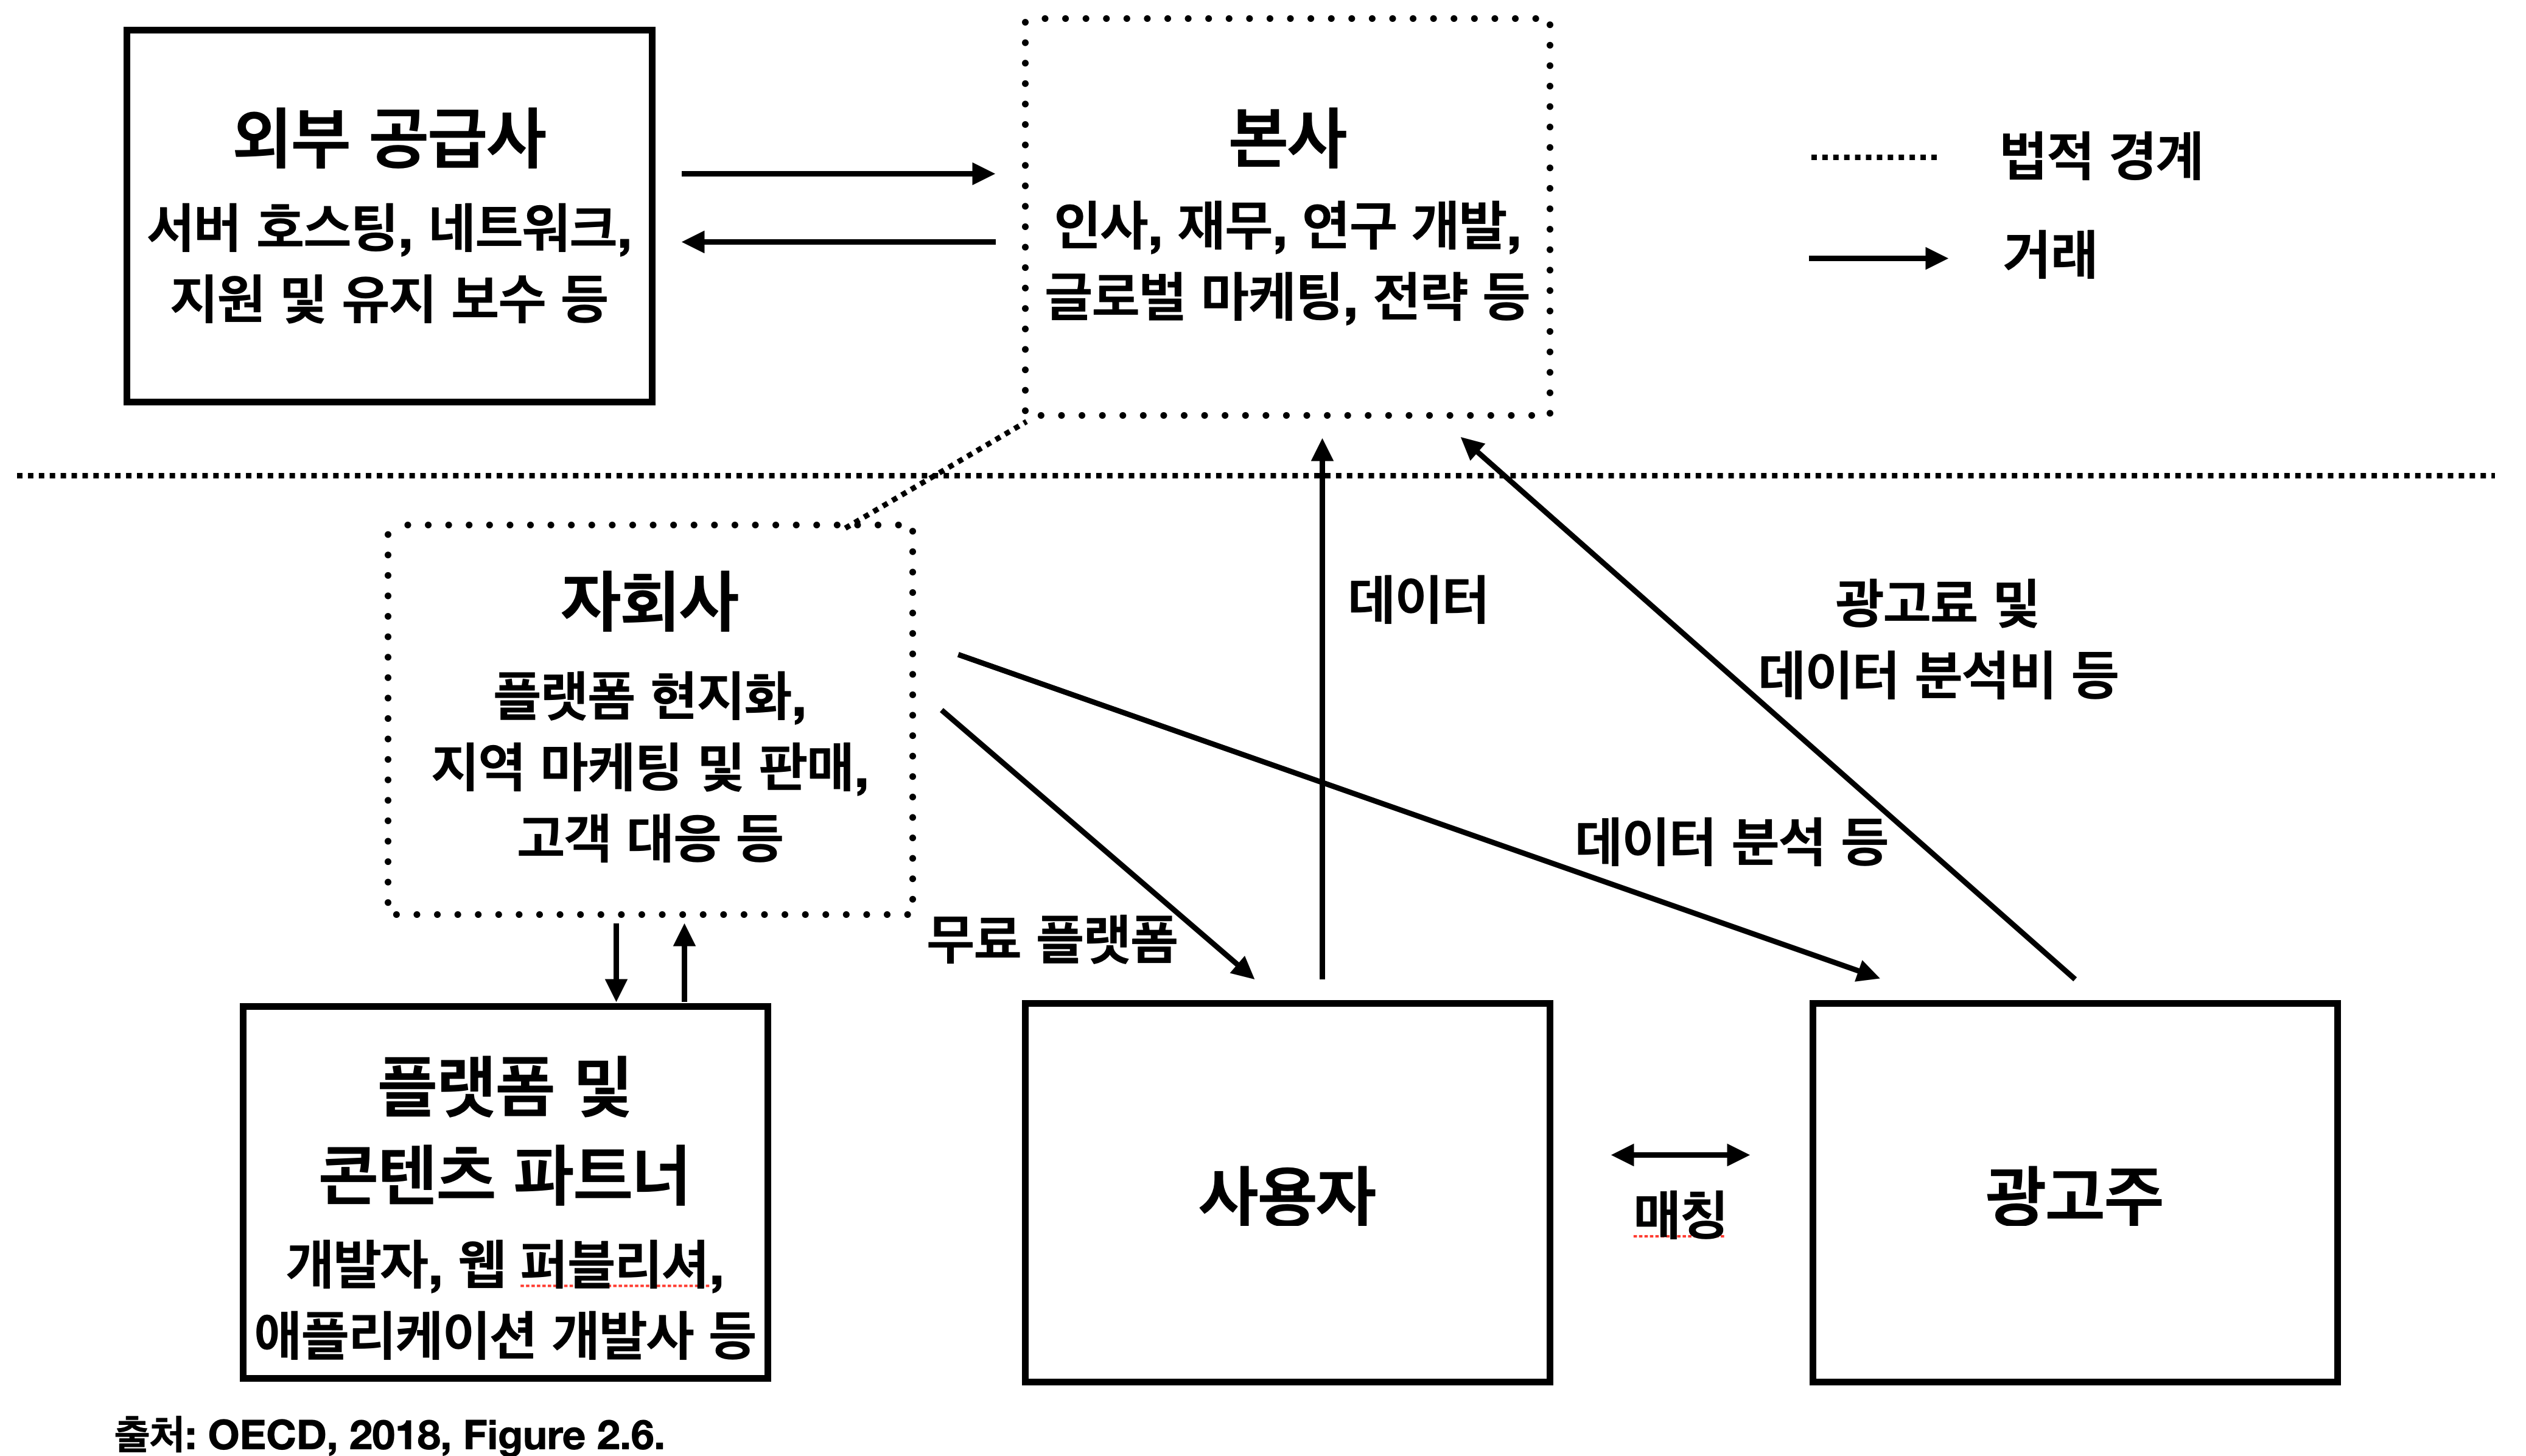
\includegraphics[scale=0.15]{schema.png}
				\caption{광고 기반 플랫폼 사업의 운영 개념도}
				\label{fig:schema}
				\end{center}
				\end{figure}		
			
		\item 또한, 광고 기반 플랫폼 사업의 경우, 광고주가 외국 기업이고, 외국 기업이 국내에 고정사업장을 두지 않은 플랫폼 사업자에게 지급하는 대가를 국내 원천 소득으로 볼 수 있는 근거가 조세 조약 및 국내세 법에 명시되어 있지 않음
		\item 다른 한 편, 플랫폼 사용자가 플랫폼에 개인 데이터를 대가로 지불한다고 보면, 개인의 거주지 국가가 이에 대해 과세권을 행사할 수 있다는 주장도 있음
		\end{itemize}
	\item 정상거래원칙(arm's length principle)에 근거한 무형 자산(지적재산권 등)에 대한 과세
				\begin{figure}[htbp]
				\begin{center}
				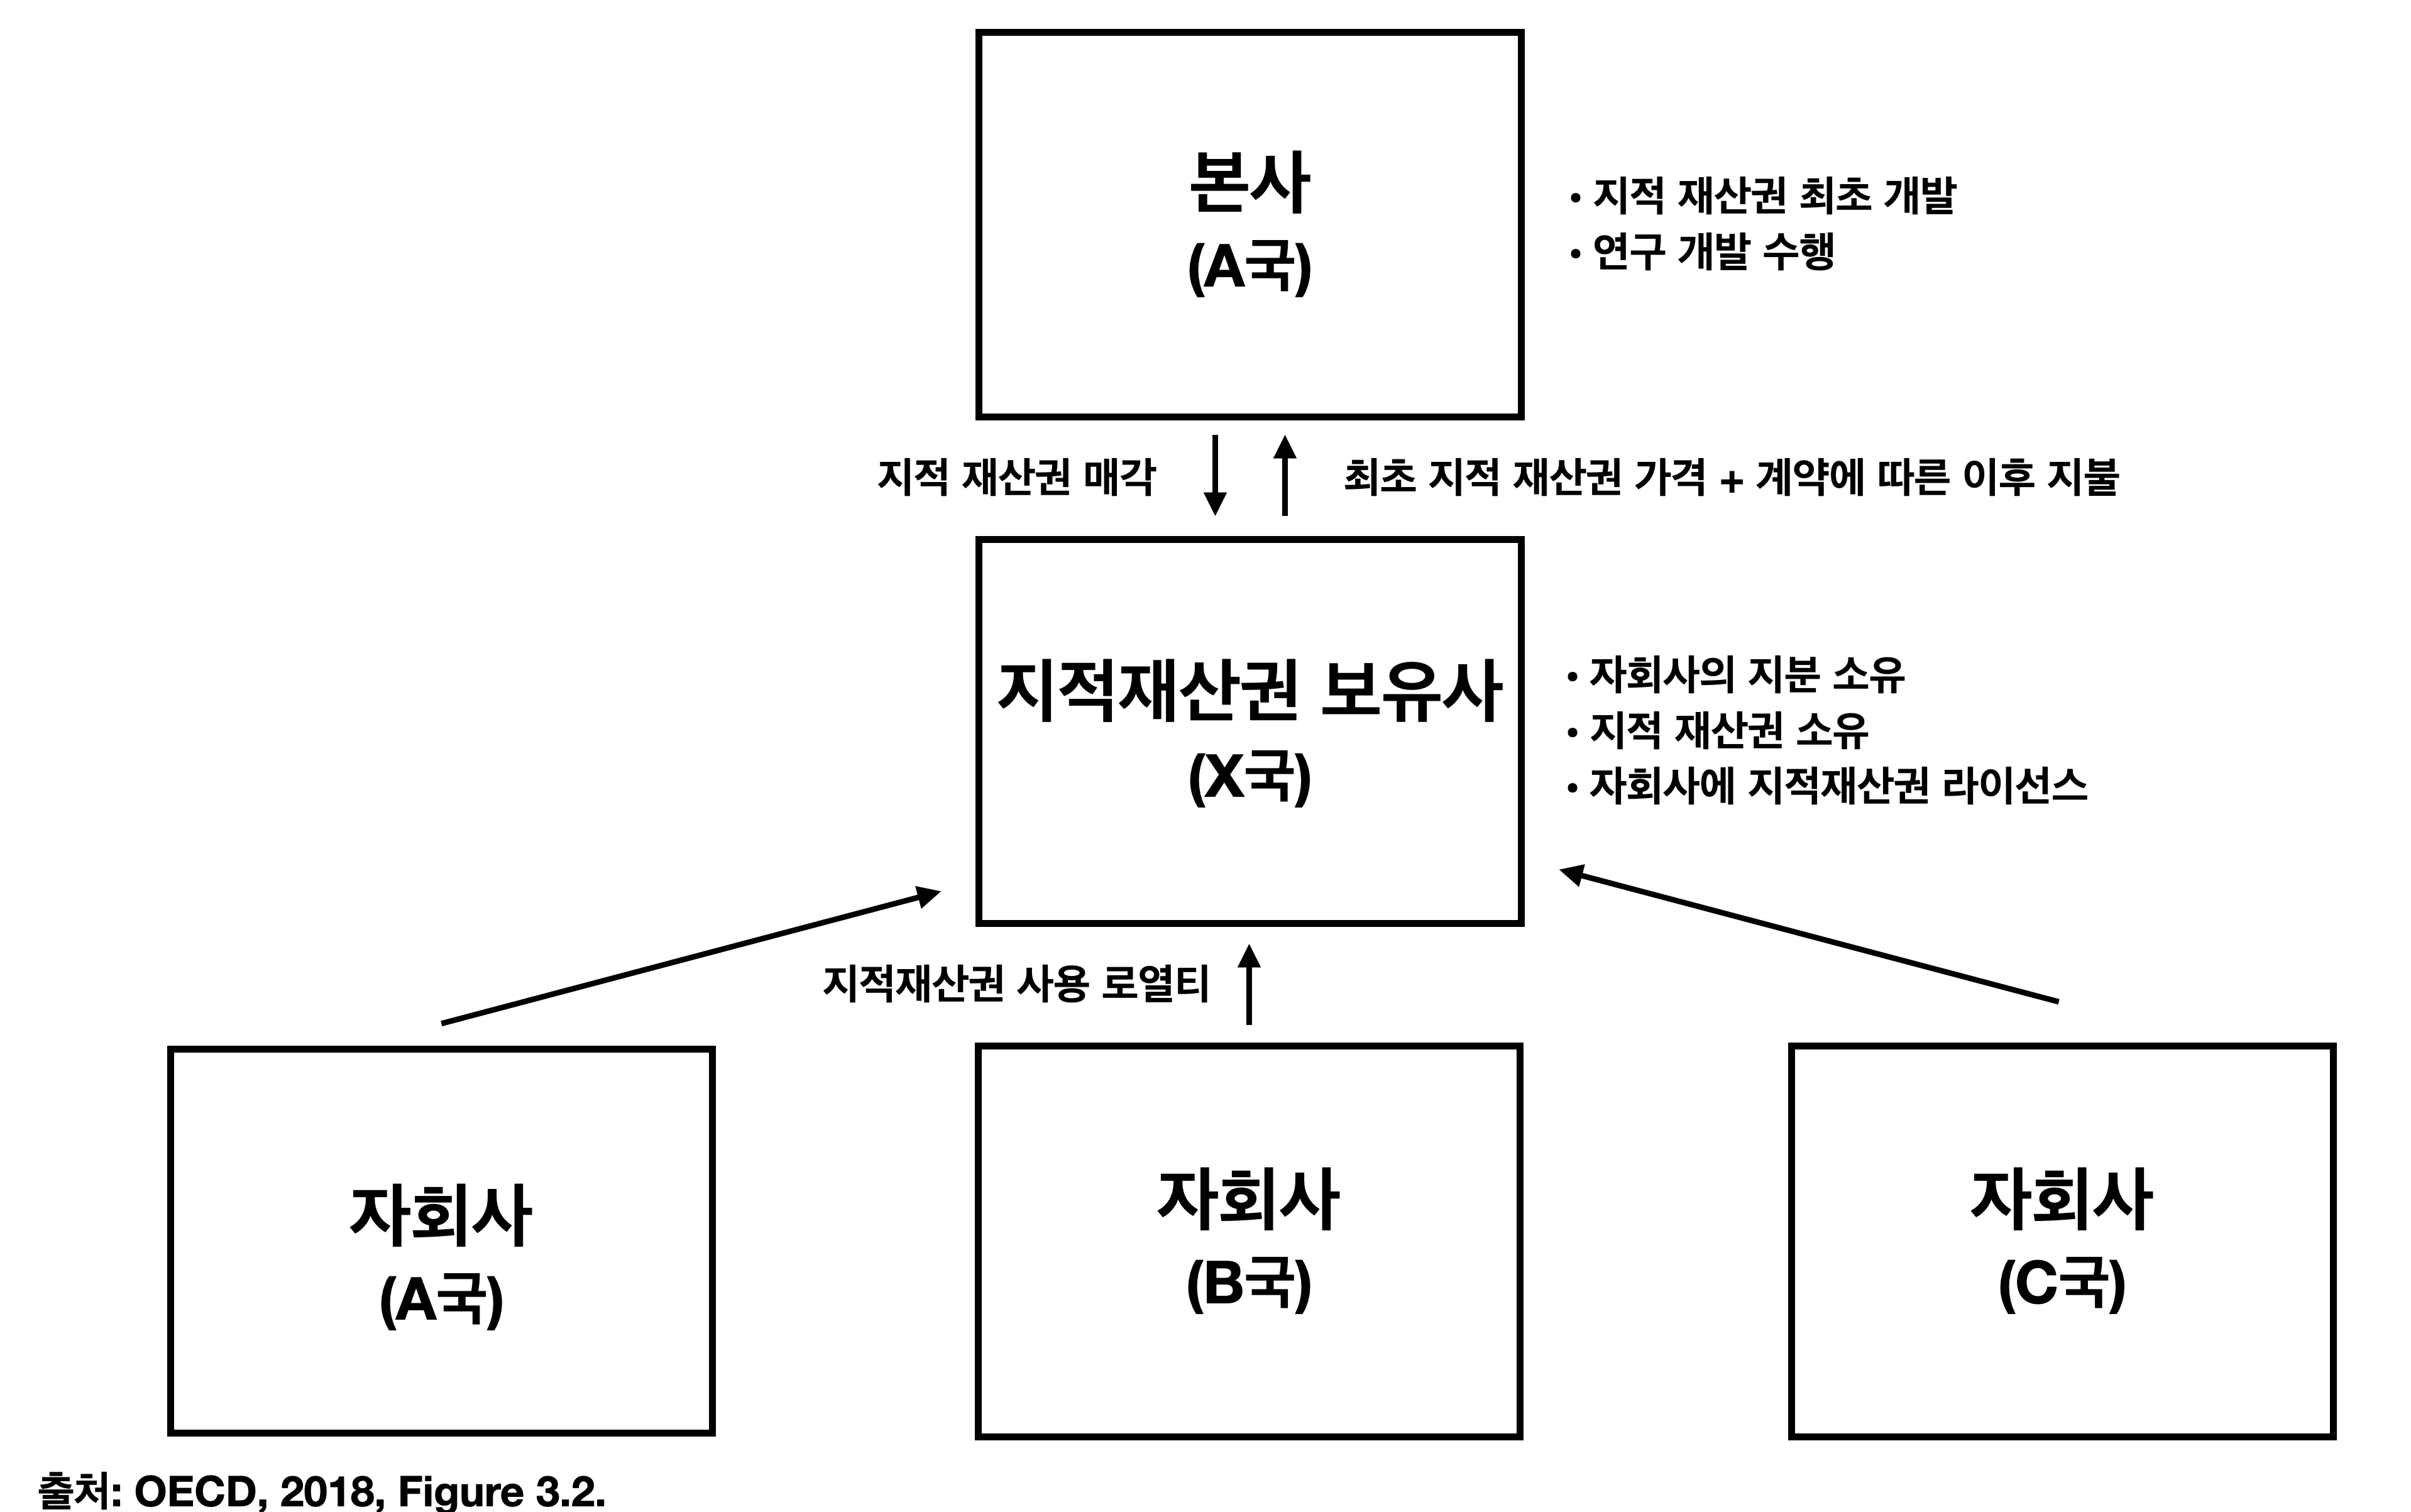
\includegraphics[scale=0.15]{schema2.png}
				\caption{로열티 수입 기업의 운영 개념도}
				\label{fig:schema}
				\end{center}
				\end{figure}	
		\begin{itemize}
		\item 국제적 조세 회피 $\rightarrow$ 즉, 소득 발생지 국가에 최소한의 사업 기능과 자산 및 위험만 두고, 그 외는 저세율 국가에 설립한 계열 회사로 이전하여, 계열 회사에 전세계에서 발생하는 소득을 유보시킴
			\begin{itemize}
			\item $\rightarrow$ 소득 발생지 국가의 세원 잠식, 과세소득의 해외 이전 발생
			\end{itemize}
		\item 혼성금융상품이나 혼성사업체를 이용한 국제적 이중 비과세 기법을 사용해 소득 발생지 국가에서의 세율을 낮추고 소득을 저세율 국가로 이전시키는 기법도 있음	
		\item 본사(A국)에서 지적재산권을 개발하고, 이를 조세율이 낮은 국가(X국)에 설립한 기업으로 이전하는 등, 이자, 배당, 사용료, 유가증권 양도소득 등에 대한 조약을 활용하여 조세 조약 상 소득 발생지 국가에서 원천징수를 할 수 없도록 되어 있는 국가에 회사를 설립하고 소득이 이 회사로 유입되도록 거래 구조를 변경
		\end{itemize}	
	\item 부가가치세(VAT: value added tax)의 국가간 형평성 저해
		\begin{itemize}
		\item 디지털 플랫폼 사업자가 소비자에게 원격으로 서비스를 공급하는 경우, 해외 공급자는 국내에서의 부가가치세를 부담하지 않을 수 있음
		\item 우리나라의 경우, 2015년 7월 이후 국내 사업장이 없는 외국 법인이 국내에 전자 서비스를 제공하는 경우 외국법인에 부가가치세를 과세할 수 있도록 함
		\end{itemize}	
	\end{itemize}
\end{itemize}

\section{디지털세 도입 논의}\label{sec:}
\begin{itemize}
\item 2012년 6월 G20 정상회담 및 재무장관 회의 이후 다국적 기업의 조세회피를 해결하기 위한 국제적 공동 대응이 주요 의제가 됨\footnote{이 절의 내용은 \cite{gimbichmalo-igyeong-geun:2019aa}, \cite{OECD/G20-Base-Erosion-and-Profit-Shifting-Project:2021uo}, \cite{yesangjun-otaehyeon:2021aa} 참고}
\item 2013년 OECD/G20 BEPS 프로젝트(Base Erosion and Profit Shifting Project)로 발전
	\begin{itemize}
	\item 2016년 2월 이후, OECD/G20 국가 외에도 전세계 140개국 참여
	\end{itemize} 
\item 2015년 11월 OECD/G20 BEPS 행동 계획 (BEPS Action Plan) 발표
	\begin{itemize}
	\item 디지털 경제에서의 조세 문제에 대한 특별한 권고 사항이 없었음
	\item $\rightarrow$ 주요 대상 기업이 누락됨에 따라 국제적 논의가 더 이상 진척되지 못함
	\end{itemize}
\item 2017년 3월, G20 재무장관 회의, 독일 주도로 	2018년까지 OECD/G20 BEPS 중간보고서 발간 결정
	\begin{itemize}
	\item 미국의 거대 기술 플랫폼 기업에 대한 유럽의 대응 논의
	\item 2017년 9월, 프랑스, 독일, 이탈리아, 스페인 등을 중심으로 균등세를 도입하자는 공동성명 발표
	\end{itemize}
\item 2018년 EU 집행위원회는 EU 차원의 디지털 세 입법을 추진
	\begin{itemize}
	\item $\rightarrow$ 회원국 간 의견 차이로 합의 실패	
	\item $\rightarrow$ 프랑스, 이탈리아, 스페인, 헝가리, 영국은 EU와 별도로 다음의 세 가지 입장에서 디지털 세 도입
		\begin{itemize}
		\item 새로운 고정사업장 개념을 적용
		\item 디지털 관련 소득을 원천 징수 대상 소득으로 분류
		\item 매출에 대한 과세
		\end{itemize}
	\item $\rightarrow$ 2019년 미국은 이들 국가의 디지털 서비스세 도입이 미국 기업에 대한 불공정 관행에 해당한다고 판단하고 보복관세 부과를 결정
	\end{itemize}
\item 2021년 미국이 적극적으로 BEPS 논의에 참여하며, 국제 디지털 세 도입이 빠르게 진행
	\begin{itemize}
	\item 2021년 3월 31일, 미국 바이든 대통령이 2조 2,500억 달러 규모의 인프라 투자 계획(American Jobs Plan)을 발표하고, 재원 마련을 위해 글로벌 최저한세 도입을 선언
	\item 2021년 6월 4-5일,  G7 재무장관/중앙은행 총재 회의에서 주요 원칙에 대한 합의가 이루어짐
		\begin{itemize}
		\item 2021년 7월 1일, OECD/G20 IF (Inclusive Framework) 총회에서 140개국 중 134개국이 6월의 회의와 합치된 합의안을 도출
			\begin{itemize}
			\item 8월 31일까지 비동의 6개국: 에스토니아, 헝가리, 아일랜드, 케냐, 나이지리아, 스리랑카
			\end{itemize}
		\end{itemize}
	\end{itemize}
\item 2021년 10월까지, 구체적인 실행 계획과 해결되지 않은 이슈에 대한 결론을 도출하기로 함
	\begin{itemize}
	\item 적용대상 기업, 배분량 구체화, 사업구분 기준 구체화, 이중과세 제거, 의무 불이행 시 대응 방안, 저세율국 최종모회사에 대한 비용 공제 부인 규칙 적용 시 추가 세액 상한 적용 여부, 최저한세율에 대한 최종 합의, 적용 예외 대상이 되는 초기 발전 단계의 다국적 기업에 대한 기준 등
	\item 나이지리아, 스리랑카, 케냐는 개발도상국에 대한 배려 조항으로 합의를 도출할 수 있을 것으로 전망
	\item 저세율국가(에스토니아, 헝가리, 아일랜드)의 반발
	\end{itemize}	
\item 2021년 10월 8일 \citep{OECD/G20-Base-Erosion-and-Profit-Shifting-Project:2021aa}	
	\begin{itemize}
	\item 136개국의 합의 발표
		\begin{itemize}
		\item 헝가리: 자동차 공장 등 자국 내 유형 자산에 대한 저세율을 향후 10년 간 유지 가능하도록, 장기 전환 기간을 인정 받음
		\item 아일랜드: 최저한세율이 최소 15\% 이상(at least)이라는 문구를 15\%로 조정
		\item 미합의:  나이지리아, 스리랑카, 케냐, 파키스탄
		\item 22년 국내 비준 및 국내법 개정, 23년 발효 및 시행	
		\end{itemize}
	\item 기둥 1 (Pillar I) 
		\begin{itemize}
		\item 목적: 고정사업장이 없더라도 시장에서 발생하는 매출을 기준으로 과세권을 부여
		\item 업종과 상관없이 매출액과 이익률 기준 상위 다국적 기업의 초과 이익에 대해 과세할 권리(Amount A)를 매출이 발생한 시장 소재국에 배분 
			\begin{itemize}
			\item 상위 다국적 기업: 글로벌 연결매출액 200억 유로 및 이익률 10\% 이상
			\item 이익률 $=$ 글로벌 세전 이익 / 글로벌 매출액
			\item 매출액 기준은 시행 7년 후 100억 유로로 축소
			\item 채굴업, 규제된 금융업 적용 제외
			\end{itemize}
		\item 과세연계점: 해당 사법권 내(국가 내)의 수입이 100만 유로 이상 발생할 경우
			\begin{itemize}
			\item 국내총생산이 400억 유로 이하인 국가의 경우 25만 유로 이상
			\end{itemize} 
		\item 초과이익 배분 비율 25\%로 합의
			\begin{itemize}
			\item Amount A $ = $ 매출액 $\times$ (세전 이익률 - 통상 이익률) $\times$ 25\%
			\end{itemize}
		\item 매출 귀속 기준: 재화나 서비스의 최종 거래가 발생하는 시장의 소재지에서 매출이 발생했다고 간주
		\item 과세 표준: 회계 기반, 손실은 이월, 구분 회계는 예외적인 경우에 한정하여 수행	
		\item 모든 분쟁 이슈는 의무적, 강제적 분쟁 해결 절차로 조정
			\begin{itemize}
			\item 단,  분쟁 대응역량이 낮은 개발도상국에 대해서는 강제적 분쟁 해결절차를 선택적으로 적용하고, 그 대상이 되는 지는 주기적으로 재심사
			\end{itemize}
		\item 기존의 디지털 서비스 세 및 관련 유사 조치는 폐지하며 향후에도 도입하지 않음
		\item 2022년까지 실행을 위한 다자 협약을 발전시키고 2023년 발효를 목표로 함
		\end{itemize}
	\item 기둥 2 (Pillar II) 
		\begin{itemize}
		\item 목적: 글로벌 최저한세를 통해 국가 간 조세 경쟁을 막음
		\item 대상: 글로벌 (연결)매출액이 7억 5,000만 유로를 넘는 다국적 기업
			\begin{itemize}
			\item 다국적 기업의 본사 소재국은 매출액 기준과 무관하게 적용
			\item 국제 해운업 제외: 실제 이익이 아닌 선박의 순톤수와 운항 일수를 기준으로 과세 표준 산출하는 톤세 제도 적용
			\end{itemize}
		\item GloBE (Global Anti-Base Erosion Proposal) 규칙: 소득산입규칙과 비용공제부인규칙으로 구성 $\rightarrow$ 도입 국가의 국내법
			\begin{itemize}
			\item 소득 산입 규칙: 자회사의 소득이 저율로 과세되는 경우, 소득산입규칙을 갖고 있는 최종모회사 소재국에 우선적으로 납부 의무가 발생하며, 해당 법인이 제3자와 지분을 분할 소유하면(80\% 미만), 차상위 중간모회사에 소득산입규칙을 대신 적용
			\item 비용 공제 부인 규칙: 소득산입규칙에 따라 초과 세액이 배분되지 않는 경우, 저세율국(최종 모회사 소재지 포함) 구성회사에 지급금을 지불한 법인이 최저한세율과의 차이만큼 추가세액을 납부
			\item 해외 진출 초기 단계의 다국적 기업은 비용 공제 부인 규칙을 5년간 적용 예외
			\item 비용공제부인규칙 발효 시점을 2024년으로 유예
			\item 소득산입규칙과 비용공제부인규칙에 적용되는 최저한세율: 15\%
			\item GloBE 규칙의 도입은 국가별 재량에 따르나 도입 시, 합의된 규칙과 일치해야 하며, 다른 회원국이 규칙을 실행하면 모든 회원국이 이를 받아들여야 함	
			\end{itemize}
		\item 원천지 국 과세 규칙  $\rightarrow$ 양자간 조세 조약
			\begin{itemize}
			\item 저세율국 소재 국외 관계사의 이자, 사용료 등 지급금에 대해 최저한세율 9\% 보다 낮은 명목 세율 적용 시, 양자간 조세 조약에 기반하여 원천지 국에 추가 과세권 인정
			\end{itemize}
		\item 2022년까지 회원국의 관련 법 개정 후, 2023년 발효	
		\end{itemize}
	\end{itemize}
\end{itemize}

\pagebreak

\section*{정리하기}
\begin{enumerate}
\item 디지털 경제의 사업 유형은 다면 플랫폼, 재판매, 수직통합, 중간재 공급 등으로 나눌 수 있다.
\item 플랫폼 사업과 디지털화로 인해, 소득의 원천이 되는 국가에 물리적 고정사업장을 두지 않고 사법 경계를 가로질러 대단위 경제 활동이 가능해졌다. 또 소프트웨어와 알고리듬 등의 무형 재산과 데이터, 사용자 참여는 시너지 효과를 내며 사용자가 부가가치를 만들고 있다.
\item 고정사업장이 없는 경제 활동은 고정사업장 소재지국의 과세권 행사라는 원칙을 위협한다.
\item 다국적 기업은 저세율 국가에 설립한 계열 회사로 무형자산에 대한 권리를 이전시켜, 전세계적 차원의 조세 회피가 가능하다.
\item 2012년부터 다국적 기업의 조세 회피에 대한 국제적 공동 대응이 본격적으로 논의되었으며 2021년 10월 전세계 136개국이 국제 디지털세 도입에 합의하게 되었다.
\item 국제 디지털 세는 크게 두 개의 기둥으로 이루어져있으며, 하나는 고정사업장이 없더라도 시장에서 발생하는 매출을 기준으로 매출이 발생한 국가가 과세권을 갖는 것이다. 다른 하나는 글로벌 최저한세율 15\%를 도입하여 국가 간 조세 경쟁을 막는 것이다.
\item 2021년의 합의는 2022년 국가 별 비준 및 세부 협약을 발전시키고 2023년 발효를 목표로 하고 있다.
\end{enumerate}
\chapter{플랫폼과 반독점: 이론}\label{cha:antitrust}

\section*{학습개요}
현대 경쟁 정책의 기본 특징과 디지털 플랫폼 시장에서의 독점 문제를 학습한다.

\section*{학습목표}
\begin{enumerate}
\item 현대 경쟁 정책의 기본 특징을 이해한다.
\item 경쟁 제한 형태의 유형을 설명할 수 있다.
\item 디지털 플랫폼 시장의 독점화 경향을 설명할 수 있다.
\item 디지털 플랫폼 산업의 진입 장벽을 설명할 수 있다.
\item 디지털 플랫폼으로 인한 사회적 손실을 설명할 수 있다.
\item 디지털 플랫폼에 대한 규제가 필요하지 않다는 입장을 설명할 수 있다.
\end{enumerate}

\section*{주요 용어}
약탈 가격, 초기 위협의 배제, 수익 체증, 정보 비대칭, 소비자 잉여, 경쟁 약화, 혁신 지체


\pagebreak

%\section{양면 시장과 경쟁 정책}
\section{경쟁 정책의 기초}
\begin{itemize}
\item 현대 경쟁 정책의 기본 특징
	\begin{itemize}
	\item 기업의 전략적 의사 결정과 시장 구조의 동태적 변화를 확인 $\rightarrow$ 사안 별 분석
	\item 현재의 시장 구조보다 잠재적 시장 진입 가능성이 더 중요 $\rightarrow$ 정부 개입의 최소화
	\item 소비자 잉여의 감소 $\rightarrow$ 정부 개입의 근거
	\end{itemize}
\item 독점 시장의 가격과 생산량
	\begin{itemize}
	\item 완전경쟁시장과 비교해 높은 가격, 적은 생산량
	\item $\rightarrow$ 독점 시장이라고 하더라도 완전 경쟁 시장에서의 자원 배분 효율성을 달성할 수 있음
		\begin{itemize}
		\item[예)] 1차 가격 차별: 모든 소비자 각각의 지불 의사에 맞춰 차별화된 가격을 부과 
			\begin{itemize}
			\item $\rightarrow$ 단, 모든 소비자 잉여가 생산자 잉여로 흡수 
			\item $\rightarrow$ 소비자 잉여의 감소 문제는 남음
			\end{itemize}
		\item[예)] 잠재적 경쟁자: 항상 새로운 기업이 시장 진입을 할 수 있다면, 기존 독점 기업은 높은 독점 가격을 유지할 수 없음
			\begin{itemize}
			\item $\rightarrow$ 가격을 한계 비용과 같은 낮은 수준으로 유지할 수 있음
			\end{itemize}
		\end{itemize}
	\end{itemize}
\item 즉, 독점 생산자인 것이 문제가 아니라 경쟁을 제한하는 행태가 문제 \citep{Shapiro:2019aa}
	\begin{itemize}
	\item 제한 가격
		\begin{itemize}
		\item 기존 기업이 신규 기업의 시장 진입을 유도하지 않으면서 부과할 수 있는 가장 높은 가격
		\item 가정: 기존 기업의 생산 비용 $<$ 신규 기업의 생산 비용
			\begin{itemize}
			\item 기존 기업은 신규 기업에 비해 생산기술, 자원 획득, 광고, 정부 허가, 판매망, 신기술 개발 등에서 이점을 누릴 수 있기 때문
			\end{itemize}
		\item 신규 기업은 기존 기업보다 낮은 가격으로 시장 진입을 시도할 것
			\begin{itemize}
			\item  $\rightarrow$ 기존 기업은 신규 기업과 같은 수준으로 가격을 낮추어 대응
			\item $\rightarrow$ 신규 기업의 수요 감소 
			\item $\rightarrow$ 신규 기업이 시장 진입 포기
			\end{itemize}
		\end{itemize}
	\item 약탈 가격 (predatory pricing)
		\begin{itemize}
		\item 기존 기업이 일시적 이윤 감소를 감수하고 후발 기업의 시장 진입을 막은 후 다시 가격을 높이는 전략
		\item 현실적이지 않다는 반론이 있음
			\begin{itemize}
			\item 약탈 가격 전략 구사 후, 기존 기업이 감소한 이윤을 회복할 수 있을까?
			\item 기존 기업이 약탈 가격을 충분히 오랫동안 구사할 수 있는가?
			\item 약탈 가격 전략을 철회한 후 다른 신규 기업이 시장에 진입하지 않는다거나, 같은 신규 기업이 다시 시장에 진입하지 않는다는 보장이 있을까?
			\item 두 기업의 비용 구조가 유사하거나 동일하다면, 신규 기업도 약탈가격 전략을 구사할 수 있지 않을까?
			\end{itemize}
		\end{itemize}
	\item 초기 위협의 배제 (exclusion of nascent threats)
		\begin{itemize}
		\item 시장의 우월적인 지위를 이용하여, 핵심 사업을 위협할 정도로 성장할 것으로 예상되는 새로운 재화나 서비스를 배제시키는 전략
		\item[예)] 대상 기업의 인수합병, 대상 재화나 서비스의 판매 방해 등 
		\end{itemize}	
	\item 우월적 지위를 남용한 인접 시장 확장	
		\begin{itemize}
		\item 인접 시장에서 자사 상품이나 서비스를 타사 상품이나 서비스에 비해 우선 판매하는 경우
		\end{itemize}
	\end{itemize}
\item 독점의 측정
	\begin{itemize}
	\item 러너 지수 (Lerner Index) $= \dfrac{p-mc}{p}$
		\begin{itemize}
		\item 즉, 기업이 정한 가격($p$)에서 한계 비용($mc$)을 뺀 것을 가격에 대한 비율로 표시 
			\begin{itemize}
			\item $\rightarrow$ 0 $<$ 러너 지수 $<$ 1
			\end{itemize}
		\item 만약 완전경쟁시장이라면 $p = mc$ 
			\begin{itemize}
			\item $\rightarrow$ 러너 지수 $=$ 0
			\end{itemize}
		\item 독점 시장이라면 한계 비용보다 높은 가격을 정할 것이므로 $p > mc$ 
			\begin{itemize}
			\item $\rightarrow$ 러너 지수 $>$ 0
			\end{itemize}
		\item 만약 이윤 극대화를 추구하는 기업이라면, 러너 지수는 수요의 가격 탄력성의 음의 역수가 됨
			\begin{itemize}
			\item $\rightarrow$ 한계 비용을 관찰하지 않고, 가격 탄력성을 관찰하여 러너 지수를 측정할 수 있음
				\begin{align*}
				\pi & = p(q)q - c(q)q \\
				F.O.C.: \dfrac{d \pi}{d q} & = \left( \dfrac{d p}{d q} q + p \right) - \dfrac{d c}{d q}  = 0 \\
				p - mc & = - \dfrac{d p}{d q} q \quad \left( \text{정의 상 } mc = \dfrac{d c}{d q} \right) \\
				\dfrac{p - mc}{p} & = - \dfrac{d p}{d q} \dfrac{q}{p} \quad (\text{양변을 $p$로 나눠줌}) \\
				& = -1 / \left(  \dfrac{d q}{d p} \dfrac{p}{q} \right) \\
				& = - \dfrac{1}{\epsilon_{d}}
				\end{align*}
			\end{itemize}
		\end{itemize}
	\item 작지만 유의하며 비일시적인 가격 인상 (SSNIP: Small but significant and non-transitory increase in price) \citep{Johnson:1986ti}
		\begin{itemize}
		\item 1982년 미국 연방 거래 위원회(Federal Trade Commission) 제안
		\item 기업 가가 재화 A, 기업 나가 재화 B를 생산한다고 가정 
			\begin{itemize}
			\item 만약 재화 A와 재화 B가 대체재 관계에 있다면,
			\item 기업 가가 기업 나를 합병하여 가상의 독점 기업을 만든 후, 재화 A의 가격을 상승시키더라도 재화 B의 판매 증가로 수입을 늘릴 수 있음 $\rightarrow$ 기업 가는 시장을 독점할 유인이 있음
			\end{itemize}
		\end{itemize}
	\item 결정적 손실 공식 (Critical loss formulas) \citep{OBrien:2003us}
		\begin{itemize}
		\item 기업 결합 $\rightarrow$ 시장 지배력 확대 가능 $=$ 가격 상승 $\rightarrow$ 거래량 감소
			\begin{itemize}
			\item 상승한 가격은 가설적인 독점 가격 (hypothetical monopoly price)
			\item 기업 결합 이후 가격 상승이 있으리라는 또는 없으리라는 증거는 무엇인가?
			\end{itemize}
		\item 결정적 손실 분석
			\begin{itemize}
			\item 합병 이후 가격 상승으로 변화할 판매량으로 발생하는 이득($\Delta p (q+ \Delta q)$)과 손실 ( - $\Delta q (p-c)$)을 비교하면 됨
				\begin{align*}
				\Delta p (q+ \Delta q) & = - \Delta q (p-c) \\
				\dfrac{\Delta p}{q} \left( 1 + \dfrac{\Delta q} {q} \right) & = - \dfrac{\Delta q}{q} \left( \dfrac{p-c}{p} \right) \quad (\text{양변을 $pq$로 나눠줌}) \\
				- \dfrac{\Delta q}{q} & = \dfrac{\Delta p / p}{\Delta p / p+m}\text{, } \quad  m = \dfrac{p-c}{p}
				\end{align*}
			\end{itemize}	
		\item 결정적 손실 공식
			\begin{equation*}
			\text{결정적 손실} = - \dfrac{\Delta q}{q}  = \dfrac{X}{X+m}\text{, } \quad  X: X \text{퍼센트 가격 상승} = \dfrac{\Delta p}{p}
			\end{equation*}
		\end{itemize}
	\end{itemize}
\end{itemize}

\section{디지털 플랫폼의 독점화 경향}
\begin{itemize}
\item 디지털 플랫폼의 산업 구조는 독점 가능성이 높고, 시장 경쟁이 제한될 수 있음
\end{itemize}

\subsection{디지털 플랫폼의 산업 구조}
\begin{itemize}
\item 디지털 플랫폼은 다음의 이유로 하나의 기업이 시장을 지배 (승자 독식, Winner takes all markets)할 가능성이 높음 \citep{Zingales:2019aa, Furman:2019wl, OECD:2018wd}
	\begin{itemize}
	\item $\rightarrow$ 시장 내에서의 경쟁이 아니라, 시장 자체의 경쟁
	\end{itemize}	
\item 네트워크 효과
	\begin{itemize}
	\item 임계 질량과 네트워크 효과: 많은 수의 사용자에서 안정, \ref{cha:networktheory}장, 그림 \ref{fig:criticalmass} 참고
	\item $\rightarrow$ 충분한 사용자 수를 확보하기 위해 초기의 집중적인 투자가 필요
	\end{itemize}
\item 규모의 경제와 범위의 경제	
	\begin{itemize}	
	\item 규모의 경제(economies of scale): 높은 고정 비용과 낮은 한계 비용
		\begin{itemize}
		\item $\rightarrow$ 초기 투자로 많은 사용자 수를 확보하고, 좋은 상품 또는 서비스를 대량으로 공급
		\end{itemize}
	\item 범위의 경제 (economies of scope): 판매하는 상품이 다양하고, 서비스의 범위가 넓을 수록 비용 하락
		\begin{itemize}
		\item $\rightarrow$ 관련 시장으로 확장
		\item[예)] 지도 검색 $\rightarrow$ 식당 추천 
		\end{itemize}
	\end{itemize}
\item 데이터 사용에 대한 수익 체증
	\begin{itemize}
	\item 수익 체증(Increasing returns to scale):  $F(aK, aL) > a F(K, L)$ 즉, 늘어난 투입량보다 더 큰 비례로 생산량이 증가
	\item 데이터를 더 많이 확보하고 활용할 수록, 관련 상품이나 서비스는 더 좋아짐
	\end{itemize}
\item 전세계 시장으로의 낮은 운송 비용
	\begin{itemize}
	\item 여기서 운송은 온라인을 통한 디지털 전송 등을 포함
	\item 소비자가 인터넷 접속이 가능해야 한다는 점, 컨텐츠 사용 등의 라이센스 등 법적 사항, 언어 장벽 등의 문제가 있음
	\item 그럼에도 불구하고 기존 사업에 비해 전세계 시장 진출 비용은 낮다고 할 수 있음
	\end{itemize}
\end{itemize}

\subsection{디지털 플랫폼의 진입 장벽}
\begin{itemize}
\item 네트워크 효과와 규모의 경제
	\begin{itemize}
	\item 신규 기업이 기존 기업만큼의 사용자 수를 확보하는 데 시간과 비용이 필요
	\item 높은 고정 비용을 부담할 수 있는 기업만 진입 가능
	\item 데이터 구축의 부담
	\item $\rightarrow$ 시장에 먼저 진입한 기업의 작은 이득이 큰 장점으로 증폭될 수 있음
	\end{itemize}
\item 소비자 행동
	\begin{itemize}
	\item 소비자는 미래 가치보다 현재 가치를 과대 평가하는 경향이 있음 \citep{Thaler:2018aa}
		\begin{itemize}
		\item[예)] 첫 번째 검색 결과나 홈페이지 가장 위의 결과를 클릭
			\begin{itemize}
			\item 즉, 다른 검색 페이지나 홈페이지의 다른 내용을 보지 않음
			\item $\rightarrow$ 플랫폼 기업은 콘텐츠가 제시되는 화면을 통제
			\end{itemize}
		\item[예)] 소비자는 개인 정보 사용에 쉽게 동의
			\begin{itemize}
			\item 플랫폼 기업이 개인 정보의 사용 내역이나 사용 방법을 구체적으로 제시했다면 동의하지 않았을 수도 있음
			\item 또는 플랫폼 기업이 개인 정보 사용 동의를 기본으로 하고, 동의하지 않는 경우에만, 즉 소비자 입장에서는 추가적인 절차($=$ 비용)를 거쳐야만 사용하지 않도록 할 수도 있음
			\end{itemize} 
		\end{itemize}
	\item 하나의 플랫폼만 사용하는 소비자 (single-homing)
		\begin{itemize}
		\item[예)] 하나의 검색엔진만 사용, 하나의 소셜 네트워크 서비스만 사용 등
		\end{itemize}	
	\end{itemize}
\item 기존 플랫폼 기업이 만든 진입 장벽
	\begin{itemize}
	\item 정보 비대칭의 활용
		\begin{itemize}
		\item[예)] 맛집 검색: 기존 플랫폼이 신규 진입 기업의 콘텐츠와 비교하기 어렵게 할 수 있음
		\item $\rightarrow$ 기존 플랫폼은 소비자가 다른 서비스를 사용하는 전환 비용을 파악하기 어렵게 함
		\end{itemize}
	\item 신규 진입 기업이 가격으로 경쟁하기 어려울 수 있음
		\begin{itemize}
		\item[예)] 기존 플랫폼 기업이 제공하는 상품이나 서비스가 무료인 경우, 이 보다 낮은 가격으로 신규 기업이 시장에 진입할 수 없음
		\end{itemize}	
	\item 기술적으로는 선도 기업이 폐쇄성을 고집하거나, 기술 호환성을 제한하거나, 데이터 이동성을 낮출 유인이 있음
	\end{itemize}
\end{itemize}

\section{디지털 플랫폼과 사회적  손실}
\begin{itemize}
\item 독점과 일반적인 사회적 손실\footnote{거대 독점 디지털 플랫폼 기업과 관련된 사회 정치적 문제, 예를 들어, 소비자 사생활 보호, 데이터 보안, 혐오 발언, 가짜 뉴스 등도 분명 중요한 이슈이지만, 이 장과 다음 장에서는 경제적인 문제에 초점을 맞춘다.}
	\begin{itemize}
	\item 소비자 잉여 손실, 경쟁 약화, 혁신 지체
	\item 디지털 플랫폼에서도 나타날까?
	\end{itemize}
\item 추천 알고리듬
	\begin{itemize}
	\item 확증 편향 (confirmation bias): 기존의 믿음 또는 가설에 맞는 정보를 찾거나, 해석하거나, 선호하거나, 되새기는 경향
	\item $\rightarrow$ 플랫폼의 추천 알고리듬이 이윤 극대화를 목표로 설계되었을 때, 
	\item (알고리듬이 의도하지 않았더라도) 충동 구매, 가격 비교 중단, 구매 중독 등의 상태를 유지하도록 유도할 수도 있음 \citep{Allcott:2020wv,Allcott:2021vp}
	\item 구매 시점을 파악하여 추천 상품이나 서비스를 제공할 수도 있음
	\end{itemize}
\item 광고 알고리듬
	\begin{itemize}
	\item 플랫폼은 광고주가 목표로 하는 대상에 대해 광고를 할 것으로 계약을 체결 
		\begin{itemize}
		\item $\rightarrow$ 그러나 많은 경우, 이러한 광고를 집행하는 알고리듬은 그 투명성이 부족
		\item $\rightarrow$ 또한 광고 가격 결정 알고리듬이 공개되지 않는 경우가 많음
		\end{itemize}
	\item 다른 한편, 플랫폼은 사용자가 더 많은 광고에 노출되도록 플랫폼에 더 많은 시간 동안 머물러 있도록 할 유인이 있음
		\begin{itemize}
		\item $\rightarrow$ 경쟁 플랫폼 또는 서비스의 사용을 막기 위한 노력
		\end{itemize}
	\end{itemize}
\item 통상적인 소비자 잉여 측정이 어려움
	\begin{itemize}
	\item 많은 경우, 사용자는 무료로 서비스를 이용 $\leftrightarrow$ 하지만, 사실 상, 화면에 대한 집중 및 개인 정보와 교환
	\item $\rightarrow$ 무료이고 품질을 관찰하기 어려운 경우, 소비의 사회적 가치($=$ 소비자 잉여)를 측정하기 어려움
	\end{itemize}
\item 플랫폼, 특히 기술 플랫폼은 보완재의 이윤을 수취
	\begin{itemize}
	\item[예)] 애플과 구글은 운영체제를 제공하고 어플리케이션 스토어를 운영하면서, 판매 수입의 30\%를 수수료로 받음
	\item[예)] 구글은 검색 엔진을 제공하고 기사를 연결하면서 광고 수입을 얻지만 최근에 와서야 뉴스를 제공하는 기업과 콘텐츠 이용 계약을 체결
	\item 플랫폼 기업과 보완재를 판매하는 기업의 관계는 동태적
		\begin{itemize}
		\item 플랫폼 서비스의 초창기에는 상호 보완적: 플랫폼 기업은 사용자를 유인할 상품이나 서비스가 필요, 보완재 기업은 더 많은 소비자에게 접근 가능
		\item 소비자가 늘어남에 따라 보완재 기업은 투자를 늘릴 수 있음 $\rightarrow$ 하지만 투자로 인한 수입이 0이 된다면 투자를 하지 않을 것
		\item $\rightarrow$ 즉, 보완재 기업이 자신이 만드는 이윤의 대부분이 플랫폼 기업의 것이 된다고 판단한다면 더 이상의 투자는 발생하지 않게 됨
		\item $\rightarrow$ 하지만, 보완재 기업이 플랫폼 기업으로부터 독립할 수 없는 상태가 되었을 수 있음
		\end{itemize}
	\end{itemize}
\item 기술 혁신 양상의 변화
	\begin{itemize}
	\item 기존 플랫폼 기업이 갖고 있는 데이터, 기술적 장점 등을 뛰어 넘을 수 없다고 예상한다면, 투자자는 새로운 기술 기업에 투자하지 않을 것
		\begin{itemize}
		\item 기존 플랫폼 기업이 보유하고 있는 데이터의 공개 여부가 중요한 역할을 할 수 있음
		\end{itemize}
	\item 기존 플랫폼 기업이 새로운 기술 기업을 인수할 것으로 예상한다면, 투자자는 새로운 기술 기업에 투자할 것
	\item $\rightarrow$ 즉, 시장을 장악해서 얻는 이윤이 아니라 인수합병에서 발생하는 이윤이 될 것
	\end{itemize}
\item 규제가 필요하지 않다는 입장
	\begin{itemize}
	\item 동태적으로 경합성이 충분하므로 사후 규제만으로 충분
	\item 플랫폼 기업간 경쟁, 온라인과 오프라인 기업 간 경쟁이 있음
	\item 플랫폼 기업에 의한 소비자 후생 감소, 데이터 우위의 중요성, 동태적 경쟁/혁신 감소의 실증적 증거는 부족한 상태 
	\end{itemize}	
\end{itemize}


\pagebreak

\section*{정리하기}
\begin{enumerate}
\item 현대 경쟁 정책의 기본 방향은 기업의 전략적 의사 결정과 시장 구조의 동태적 변화를 고려하여 사안 별 분석, 잠재적 시장 진입 가능성을 검토함으로써 정부 개입을 최소화, 정부 개입은 소비자 잉여의 감소에 근거하는 특징을 갖고 있다.
\item 경쟁을 제한하는 행태가 중요한 문제점이고, 이에 해당하는 기업 전략은 약탈 가격, 초기 위협의 배제, 우월적 지위를 남용한 인접 시장 확장 등이 대표적이다.
\item 디지털 플랫폼은 네트워크 효과, 규모의 경제, 범위의 경제, 데이터 사용에 대한 수익 체증, 전세계 시장으로의 낮은 운송 비용으로 독점화 경향이 강하다.
\item 네트워크 효과와 규모의 경제로 인해 디지털 플랫폼 산업의 진입 장벽이 있으며, 소비자 행동, 기존 기업의 정보 비대칭 활용, 기술 및 데이터 호환성 전략도 진입 장벽으로 작동한다.
\item 디지털 플랫폼의 추천 알고리듬이나 광고 알고리듬은 각각 확증 편향으로 인한 비합리적 소비 유인과 플랫폼 이용 시간 등의 증가로 소비자 잉여를 감소시킬 가능성이 있다.
\item 또한, 플랫폼은 보완재 판매의 이윤을 수취하며 이로 인해 보완재 기업의 투자를 가로막을 수 있고, 기술 혁신의 목표도 시장 장악이 아니라 인수합병의 이윤 취득으로 바뀌게 됨에 따라 기술 혁신을 가로 막을 가능성도 높다. 
\item 그럼에도 불구하고, 시장의 동태적 경합성이 있음, 플랫폼 기업 간 경쟁 및 온라인과 오프라인 간 기업의 경쟁이 있음, 플랫폼 기업에 의한 사회적 잉여 감소의 실증적 증거 부족을 근거로 디지털 플랫폼 기업에 대한 규제가 필요하지 않다는 입장도 있다.
\end{enumerate}
\chapter{플랫폼과 반독점: 현실과 정책}\label{cha:competitionpolicy}

\section*{학습개요}
거대 기술 기업의 반독점 혐의를 살펴보고, 이를 규제하기 위한 노력을 학습한다.

\section*{학습목표}
\begin{enumerate}
\item 현재 경쟁 정책의 플랫폼 산업에 대해 갖는 한계를 설명할 수 있다.
\item 거대 기술 기업에 대한 규제 방향을 설명할 수 있다.
\end{enumerate}

\section*{주요 용어}
경쟁 제한, 이해관계 충돌, 비차별 원칙, 데이터 이동성

\pagebreak

\section{플랫폼 기업의 현실}\label{sec:}
\subsection{플랫폼 기업 현황}
\begin{itemize}
\item GAFA \citep{Liaubet:2021tz}
	\begin{itemize}
	\item Google, Apple, Facebook, Amazon
	\item 2020년 현재, 네 기업의 매출 총합은 터키의 국내총생산에 맞먹음
	\item 의료, 게임, 영상, 음악, 지불, 커뮤니케이션, 운송 등 다방면의 사업
	\item 지난 2018--2020년 간, 네 기업이 인수합병한 기업은 모두 58개, 15억 5,900만 달러, 평균 2천 687만 달러
		\begin{itemize}
		\item 같은 기간, 미국 주식시장 에스엔피 500 (S\&P 500) 기업 중 1,000만 달러 이상의 인수는 3건
		\end{itemize}
	\end{itemize}
\item 2016--2019, 전세계 43개국, 마켓플레이스 등 특정 산업, 웹사이트 통신량(traffic) 기준 \citep{Costa:2021up}
	\begin{itemize}
	\item 대상 국가
		\begin{itemize}
		\item 2013--2014년: 아르헨티나 등 23개국
		\item 2015년: 헝가리 등 3개국 추가
		\item 2016--2019년: 한국 등 17개국 추가
		\end{itemize}
	\item 산업
		\begin{itemize}
		\item 마켓플레이스 소비자 대상 (X2C), 241개, 아마존(amazon), 이베이(ebay) 등
		\item 마켓플레이스 비즈니스 대상 (B2B), 115개, 알리바바(alibaba), 인디아마트(indiamart) 등
		\item 레스토랑 예약: 46개, 오픈테이블(opentable), 조마토(zomato) 등
		\item 레스토랑 배달: 149개, 딜리버루(deliveroo), 우버이츠(ubereats) 등
		\item 운송: 85개, 우버(uber), 그랩(grab) 등
		\item 숙박: 210개, 에어비앤비(airbnb), 부킹닷컴(booking.com) 등
		\item 전문 서비스: 컴퓨터 프로그래밍, 법률/회계, 건축 및 공학 등, 광고 및 시장 조사, 기타 전문 및 과학 기술 활동, 147개, 업워크(upwork), 프리랜서(freelancer) 등
		\item 개인 서비스: 특수 건축 활동, 건축 및 조경 활동, 컴퓨터와 개인 및 가구 재화 수리, 기타 개인 서비스 활동 등, 185개, 트리트웰(treatwell), 태스크래빗(taskrabbit) 등
		\item 모바일 지불: 150개, 페이팔(paypal), 라쿠텐(rakuten) 등
		\end{itemize}
	\item 총 플랫폼의 수와 1인당 플랫폼 웹사이트 통신량은 증가 중
	\item 하지만, 산업별, 국가별 큰 차이가 있음
	\end{itemize}
\end{itemize}

\subsection{거대 기술 기업의 반독점 혐의}\label{sec:}
\begin{itemize}
\item 페이스북 \citep{Subcommittee-on-Antitrust-Commercial-and-Administrative-Law:2020aa}
	\begin{itemize}
  \item 경쟁 회피 또는 경쟁자 제거를 목적으로 인스타그램, 왓츠앱을 포함하여 스타트 업 인수를 논의한 내부 이메일 확인
  \item 시장 우월적 데이터를 활용 잠재적 신규 기업을 확인하고, 관련 기업을 인수, 모방, 운영 중단시킴
	\end{itemize}	
\item 아마존
	\begin{itemize}
	\item 아마존 마켓플레이스를 이용하는 상당수의 중소 기업이 다른 대안이 없으므로 시장 지배력을 행사하고 있는 것으로 인정해야 함
  \item 성장 과정에서 다이어퍼스, 자포스(Diapers.com, Zappos) 등의 온라인 소매 기업을 인수
	\begin{itemize}
	\item $\rightarrow$ 기업뿐만 아니라 사용자도 인수함으로써 시장 지배력을 강화함
	\end{itemize}
  \item 내부 문서에 따르면, 마켓플레이스를 이용하는 판매자를 내부 경쟁자로 호칭
	\begin{itemize}
	\item $\rightarrow$ 직접 판매자이자 시장 관리자인 아마존의 이중적 지위로 볼 때, 이해관계의 충돌이 발생 
	\item $\rightarrow$ 판매자 정보에 대한 접근력을 활용할 유인이 됨
	\end{itemize}
  \item 성장 중인 음성 인식 시장에서 고착 효과를 누리고 있음
		\begin{itemize}
		\item 고착 효과(lock-in effect): 높은 전환 비용(switching cost)으로 다른 상품이나 서비스로 전환할 수 없음
		\end{itemize}
	\item 아마존 웹 서비스는 아마존과 경쟁 중인 다른 기업에 중요한 인프라를 제공하고 있어, 잠재적인 이해관계 충돌 가능성이 높음
		\begin{itemize}
		\item $\rightarrow$ 경쟁자에게 최적의 기술을 제공하지 않을 가능성이 있음
		\end{itemize}
	\end{itemize}	
\item 애플
	\begin{itemize}
 	\item 모바일 기기 운영 체제 시장에서 시장 지배력을 행사하고 있음
		\begin{itemize}
		\item $\rightarrow$ 높은 전환 비용, 높은 진입 장벽, 네트워크 효과로 인해 시장 지배력을 유지
		\item 경쟁 제한을 위한 장벽, 자사가 제공하는 서비스를 우선함으로써 경쟁자를 차별
		\end{itemize}
	\item 경쟁과 관련된 민감한 정보를 부적절하게 활용함으로써 앱 개발자를 차별
	\item 독점적 지위를 이용 앱 스토어 내에서 초 경쟁 가격을 부과
	\item 하드웨어 판매에서 더 많은 수입을 얻고 있지만, 앱스토어의 수수료가 수입에서 차지하는 비중이 빠르게 늘어나는 중
		\begin{itemize}
		\item $\rightarrow$ 앱스토어에서의 경쟁 약화는 앱의 혁신과 품질 향상을 가로 막고, 가격 상승과 소비자 선택의 폭을 좁히는 결과를 가져 올 것
		\end{itemize}
	\end{itemize}	
\item 구글
	\begin{itemize}
	\item 검색 시장의 독점력을 이용하여 제 3자에게 부적절한 콘텐츠를 제시하고, 구글의 열등한 수직 상품을 제공
		\begin{itemize}
		\item $\rightarrow$ 제3의 수직 공급자를 상대적으로 낮은 위치로 내림
		\end{itemize}
	\item 일반 검색의 독점력을 활용, 유료 광고 검색과 일반 검색의 경계를 흐리게 만들어, 광고 및 구글 자체의 콘텐츠를 검색 결과 페이지에 제공
	\item 스마트폰 제조사가 안드로이드 운영체제를 사용할 때, 구글의 애플리케이션이 사전 설치되고 기본 애플리이션으로 설정되도록 요구
	\end{itemize}
\end{itemize}


\section{경쟁 정책의 한계}\label{sec:}
\begin{itemize}
\item 경쟁 측정의 한계 \citep{Evans:2013vp,Jenny:2015wh}
	\begin{itemize}
	\item 한 집단의 수요의 가격 탄력성으로 측정 
		\begin{itemize}
		\item $\rightarrow$ 양면 시장(플랫폼)은 서로 다른 면에서의 수요에 대한 가격 탄력성이 서로 영향을 줌
		\end{itemize}
	\item 디지털 상품의 경우 한계 비용이 0에 가까움 
		\begin{itemize}
		\item $\rightarrow$ 마치 완전경쟁시장과 같은 결과
		\end{itemize}
	\item 어느 한 면의 사용자가 무료로 플랫폼의 서비스를 사용하는 경우, 결과가 왜곡됨
	\end{itemize}
\item 약탈 가격 적용의 어려움
	\begin{itemize}
	\item 아마존 등 전자 상거래 플랫폼의 경우 
	\item $\rightarrow$ 플랫폼을 이용하는 판매자를 가격 경쟁 시킴 
	\item $\rightarrow$ 소비자의 구매 가격 하락 
	\item $\rightarrow$ 약탈 가격의 논리가 성립하지 않음
	\end{itemize}
\item 우월적 지위를 남용한 인접 시장 확장	
	\begin{itemize}
	\item 아마존은 자사 상품의 판매와 동시에 전자 상거래 플랫폼을 운영
		\begin{itemize}
		\item 플랫폼 이용 판매자의 상품 모방 
			\begin{itemize}
			\item $\rightarrow$ 지적재산권 침해 문제이지 플랫폼의 문제는 아님
			\end{itemize}
		\item 홈페이지 등에서 자사 상품을 우선 배치, 판매 시 추가 비용 부담 등
			\begin{itemize}
			\item 입증이 불가능한 것은 아니지만 어려움
			\item 만약 플랫폼이 이를 하겠다고 의도하면 정교화할 것을 예상할 수 있음
			\end{itemize}
		\end{itemize}
	\end{itemize}
\end{itemize}

\section{경쟁 정책의 논의}
\subsection{유럽 연합}
\begin{itemize}
\item 디지털 시장 법(DMA: Digital Market Act) 
	\begin{itemize}
	\item 다음의 기업을 문지기(gatekeeper)로 추정 \citep{Cremer:2019aa,choegyeyeong:2020we,gimhyeonsu-gang-ingyu:2020aa}
		\begin{itemize}
		\item 적어도 3개 이상 회원국 에서 핵심 플랫폼 서비스 제공
		\item 최근 3년 회계연도에서 유럽 경제 지역(EEA: European Economic Area)에서 연간 매출액이 65억 유로 이상 또는 지난 1년 간 평균 주가 총액(또는 이에 상응하는 공정 시장 가치)이 650억 유로 이상
		\item 지난 회계연도 역내 활성 이용자 월 4천 5백만명 및 사업 이용자 1만명 이상
			\begin{itemize}
			\item 또는 지난 3년 회계연도 각각에서 위 기준을 충족할 경우
			\end{itemize}
		\end{itemize}
	\item 문지기 준수 의무
		\begin{itemize}
		\item 문지기는 다른 서비스나 제 3 사업자의 개인 데이터를 결합하는 행위를 금지하고 최종 이용자가 문지기의 다른 서비스에 가입하도록 하는 요구 금지
		\item 사업 이용자에게 문지기의 식별 서비스 이용 요구를 금지
		\item 사업자 및 최종 이용자에게 문지기의 다른 핵심 서비스 이용을 요구하는 행위 금지
		\item 사업 이용자의 제 3 사업자의 중개 이용을 허용
		\item 사업 이용자가 문지기를 통하지 않고 판매를 촉진할 수 있어야 하고 이에 대한 최종 이용자의 접근 및 이용이 가능해야 함
		\item 광고주 및 광고 퍼블리셔에 가격 등 요구 정보를 제공할 의무
		\item 공공 기관을 통한 이의 제기 가능
		\end{itemize}	
	\item 조정 사항
		\begin{itemize}
		\item 사전 탑재 어플리케이션의 제거(uninstall) 허용
		\item 문지기 핵심 서비스를 통하지 않고 앱이나 앱스토어를 허용
		\item 문지기의 앱스토어에 대한 사업 이용자의 공정하고 비차별적인 접근 허용
		\item 문지기 자체 및 관련 기업 우대 자제할 것
		\item 문지기의 운영체제를 이용해 다른 서비스나 다른 앱으로의 전환 또는 구독을 기술적으로 제한하는 행위를 자제할 것
		\item 사업 이용자와 보조 서비스 제공자는 문지기 보조 서비스에 사용하는 운영체제, 하드웨어, 소프트웨어 기능에 접근하고 상호 운용 허용
		\item 사업 이용자와의 경쟁을 위해 사업 이용자 및 그 최종 이용자로부터 산출된 데이터를 이용하는 행위 자제(refrain)
		\item 광고주 및 광고 퍼블리셔 요청 시 성과 측정 도구 접근 및 독립적 검증 수행에 필요한 정보 제공
		\item 사업 및 최종 이용자 활동으로 생성된 데이터에 지속적 실시간 접근을 포함하여 데이터 이동성 및 이를 원활하게 하는 도구 제공
		\item 사업 이용자(및 사업 이용자가 승인한 제 3자)에게 최종 이용자가 제3자 핵심 서비스를 이용하는 과정에서 제공 또는 생성된 집계 및 비집계 데이터 접근을 허용
			\begin{itemize}
			\item 개인 정보는 개인의 공유 허용을 전제
			\end{itemize}
		\item 검색 엔진에서 이용자가 생성한 랭킹, 쿼리, 클릭 및 보기 데이터에 대해 경쟁 검색자의 접근 요구를 따라야 함. 단 정보의 익명화는 전제되어야 함
		\end{itemize}	
	\end{itemize}
\end{itemize}

\subsection{미국}
\begin{itemize}
\item 미 하원 보고서, 디지털 시장에서의 경쟁에 대한 조사 \citep{Subcommittee-on-Antitrust-Commercial-and-Administrative-Law:2020aa,gimhyeonsu-gang-ingyu:2021aa}
	\begin{itemize}
	\item 비차별 원칙 $\rightarrow$ 자기 우대 제한, 동일 서비스에 대한 동일 계약, 결합 판매 금지 등
	\item 인접 시장 진출 제한과 기업 분할을 포함한 거대 플랫폼 구조 조정 등
	\item 전환 비용을 낮추기 위해 상호 운용성 및 데이터 이동성을 높이기 위한 개방적 서비스 접근 촉구
	\item 시장지배적 사업자의 인수 합병을 반경쟁적 행위로 추정
	\end{itemize}
\item 후속 조치로, 미 하원, 2021년 6월 플랫폼 규제 패키지 법안 발의
	\begin{itemize}
	\item 5개의 법안
		\begin{itemize}
		\item 플랫폼 독점 종식법 (Ending Platform Monopolies Act), 
		\item 진입방해 인수합병 금지 (Platform Competition and Opportunity Act),
		\item 자사제품 특혜제공 금지법 (American  Innovation and Choice Online Act),
		\item 소셜미디어 이동제한 금지법 (Augmenting Compatibility and Competition by Enabling Service Switching Act), 
		\item 합병신청 수수료 인상법 (Merger Filing Fee Modernization Act)
		\end{itemize}
	\item 대상
		\begin{itemize}
		\item 미국 내 활성 이용자 월 5,000만명, 활성 사업이용자 월 10만명
		\item 시가 총액 6,000억 달러 이상
		\item 온라인 플랫폼에서 재화와 서비스 판매를 위한 중요한 거래 상대방
		\end{itemize}
	\item 주요 내용
		\begin{itemize}
		\item 플랫폼 제공자의 자사 재화 및 서비스 판매 중단
		\item 인수 합병의 경쟁 제한성 없음에 대한 입증 책임을 플랫폼 기업에 부과
		\item 자사 제품 우대 금지
		\item 소셜 미디어 데이터 이동성 보장 등
		\end{itemize}
	\end{itemize}
\end{itemize}

%\cite{Shapiro:2019aa}
%. A tech titan putting up obstacles to customers seeking to also use rival products could easily face liability under this precedent. As a recent example of exclusionary conduct, Facebook blocked Vine, a video sharing app launched by Twitter in January 2013, from accessing Facebook user data (O’Sullivan and Gold 2018). This prevented Facebook users from inviting their Facebook friends to join Vine. Facebook was applying its policy of restricting access to apps that replicated Facebook’s core functionality. In response to the Vine episode becoming public, Facebook stated that it was dropping this policy (Facebook 2018), which appears difficult to defend. Twitter discontinued the Vine mobile app in October 2016
%
%Apple has been accused of discriminating against rivals who rely on the Apple platform to reach consumers. In March 2019, the music streaming service Spotify filed an antitrust complaint at the European Commission against Apple (Ek 2019). 
%Spotify objected to the 30 percent fee that Apple charges on certain purchases made through Apple’s payment system and claimed that Apple had locked Spotify out of Apple Watch. Spotify asserted that it should receive the same treatment at the Apple App Store given to Apple’s competing service, Apple Music. In response, Apple claimed that it had worked closely with Spotify for years and that Spotify was not willing to abide by the same rules that apply to all apps on the App Store, which Apple regards as necessary for the operation and security of the App Store. Apple further claimed that Apple approved Spotify for the Apple Watch and that Spotify has been the leading app in the Watch Music category. The European Commission is opening an investigation in response to Spotify’s complaint.
%The Spotify complaint illustrates the tensions that arise when the company controlling a platform also offers its own services on that platform. Indeed, the boundary between the “platform” and services running on that platform can be fuzzy and can change over time. Similar issues will surely arise for other applications that rely on Apple’s App Store to reach customers. For example, Apple recently removed several parental control apps from the App Store. These apps provide alternatives to Apple’s own screen-time control tools. Apple explained that it took this action to protect users’ privacy and security, but an antitrust complaint here would not be shocking (Apple 2019).
%
%We know a lot more about what a case of this type might look like against Google, because the European Commission issued an antitrust decision in June 2017 against Google involving Google Shopping, including a €2.42 billion (\$2.7 billion) fine.9 Google displays advertisements when users enter queries into the Google search engine that relate to commercial products. For example, Figure 1 shows what one sees on a desktop computer if one searches for “Nikon Cameras” on Google. 
%All of the images displayed in Figure 1 are sponsored search results; that is, they are advertisements paid for by online merchants. Google calls these “Product Listing Ads.” A user who clicks on one of these ads is directed to the website of the online merchant sponsoring that ad, and that sponsor pays a fee to Google. The first link to NikonUSA.com is also an advertisement, in text form. The second link to NikonUSA.com is a generic search result generated by Google’s algorithm, not an advertisement. More generic search results, not shown in Figure 1, follow.
%Many press reports have left the impression that the European Commission case was about Google biasing its search algorithm by demoting its rivals, but that is not correct. The European Commission fact sheet states, “The Commission Decision does not object to the design of Google’s generic search algorithms or to demotions as such, nor to the way that Google displays or organizes its search results pages (e.g., the display of a box with comparison shopping results displayed prominently in a rich, attractive format)” (European Commission 2017). Instead, the European Commission “objects to the fact that Google has leveraged its market dominance in general internet search into a separate market, comparison shopping. Google abused its market dominance as a search engine to promote its own comparison shopping service in search results, whilst demoting those  of rivals.” According to the European Commission, Google did this by displaying Product Listing Ads, such as those shown in Figure 1. This is a peculiar claim, because those Product Listing Ads are very much like the text ads that Google has shown for years, and the European Commission does not object to ads that use text rather than images. Plus, as the European Commission recognizes, there is nothing wrong from a competitive perspective when a content provider earns revenue by selling advertisements. The newspaper and radio industries have done that for a very long time. Furthermore, it is not apparent how the Product Listing Ads “promote” Google’s comparison shopping service, since a user who clicks on one of those ads is directed to the merchant’s website, not to the stand-alone Google Shopping site.

\pagebreak

\section*{정리하기}
\begin{enumerate}
\item 플랫폼 산업에서는 각 면에서의 수요에 대한 가격탄력성이 서로 영향을 주므로, 어느 한 면에서의 가격탄력성으로 경쟁 정도를 측정하는 방법은 결과를 왜곡시킬 수 있다.
\item 플랫폼 산업에서는 병목을 향한 경쟁처럼 어느 한 면의 사용자에게 경쟁을 유도할 수 있으므로, 소비자 잉여의 감소가 나타나지 않을 수 있다.
\item 우월적 지위를 남용한 인접 시장 확장의 방법도 플랫폼에 대한 반독점 정책이 아니라 지적 재산권 침해 등 다른 정책적인 대안으로 접근해야할 경우도 있다.
\item 디지털 플랫폼 기업에 대한 유럽 연합과 미국의 반독점 정책은 플랫폼 사업자 자신과 플랫폼을 이용하는 사용자 간의 비차별, 상호 운용성 및 데이터 이동성을 높이는 기술적 대안의 의무화 등을 큰 방향으로 설계되고 있다.
\end{enumerate}
\chapter{플랫폼과 노동: 이론}\label{cha:platforminlabormarket}

\section*{학습개요}
플랫폼을 통해 중개되는 노동의 특징을 학습한다.

\section*{학습목표}
\begin{enumerate}
\item 플랫폼을 통한 노동 중개의 개념을 설명할 수 있다.
\item 디지털 기반의 플랫폼 노동 중개의 분류와 각각의 특징을 설명할 수 있다.
\item 노동에 대한 플랫폼 중개의 장점과 단점을 기업과 노동자의 입장에서 각각 설명할 수 있다.
\item 노동의 플랫폼 중개에 대한 다양한 평가를 설명할 수 있다.
\end{enumerate}

\section*{주요 용어}
온라인 웹 기반 노동 중개 플랫폼, 위치 기반 노동 중개 플랫폼, 알고리듬에 의한 관리

\pagebreak

\section{플랫폼과 노동}\label{sec:}
\begin{itemize}
\item 플랫폼 관련 노동의 유형
	\begin{itemize}
	\item 플랫폼 기업에 종사하는 노동
	\item 플랫폼을 통한 노동 중개
		\begin{itemize}
		\item 노동 의뢰인 -- 플랫폼 -- 노동자
		\item 노동자도 다시 두 부류로 나눌 수 있음
			\begin{itemize}
			\item 플랫폼 기업이 직접 고용한 노동자
			\item 플랫폼의 중개를 받아 일을 하는 노동자 $\rightarrow$ 보통, 자영업자 (self-employed)나 독립 계약자 (independent contractor)로 분류
			\end{itemize}
		\end{itemize}
		
		\begin{figure}[htbp]
		\begin{center}
		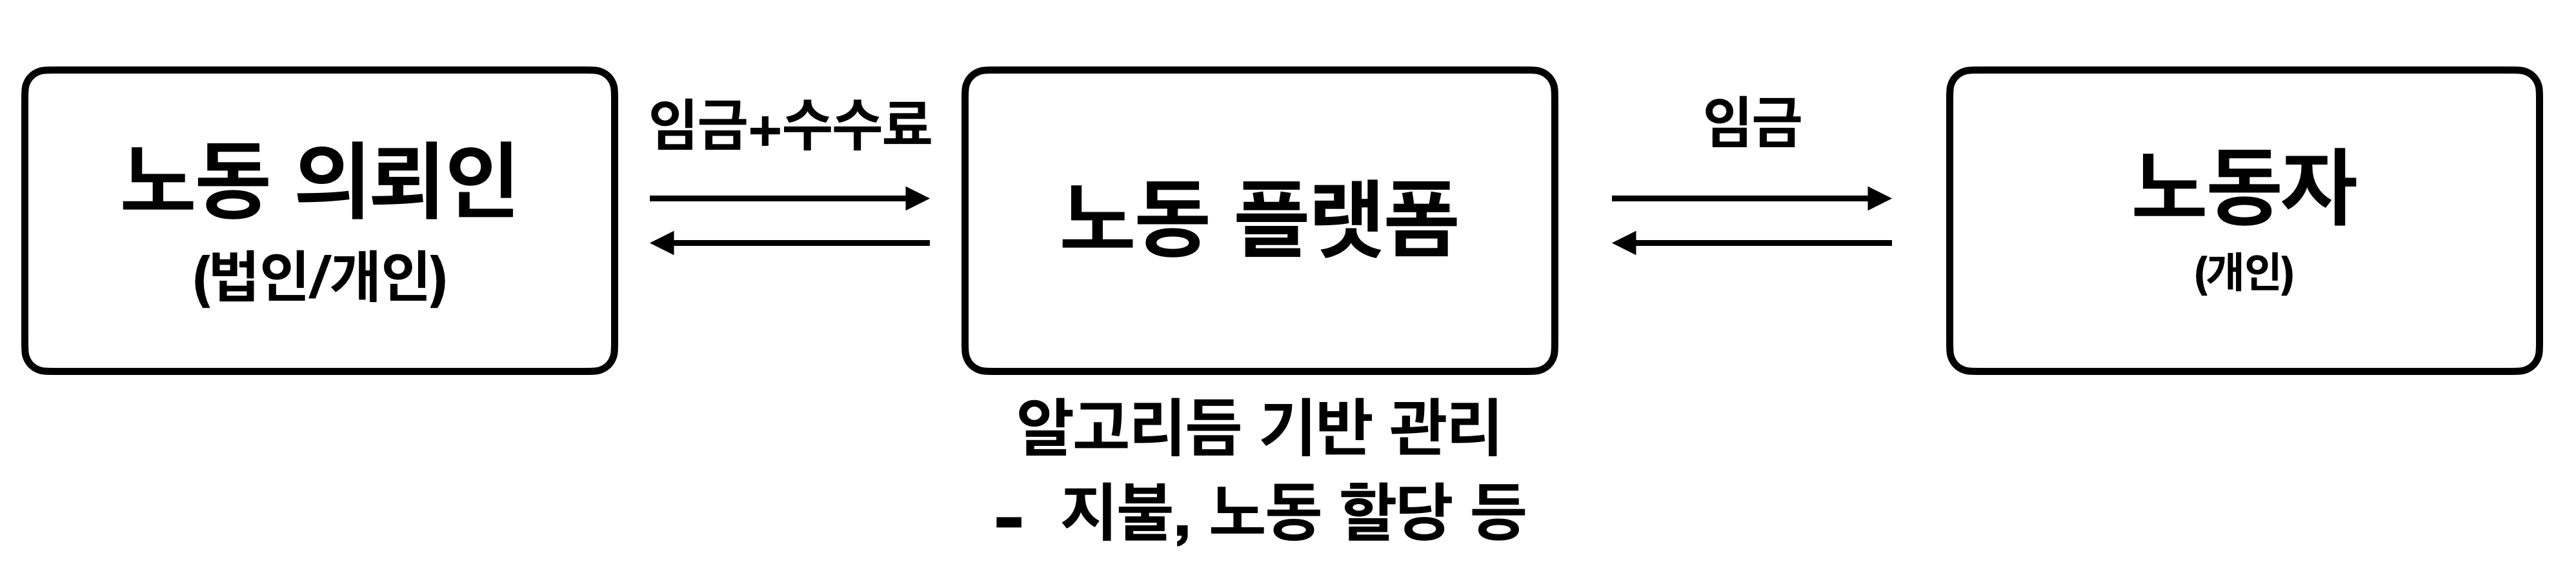
\includegraphics[scale=0.2]{platform_labor.png}
		\caption{플랫폼을 통한 노동 중개}
		\label{fig:platform_labor}
		\end{center}
		\end{figure}		
		
	\item 앞으로 다루고자 하는 것은 후자, 특히 디지털 기반의 플랫폼을 통한 노동 중개 문제
	\end{itemize}
\item 디지털 기반 플랫폼의 노동 중개 \citep{International-Labour-Office:2021uk}	 \footnote{이 외에도 \cite{Schmidt:2017ws}는 클라우드 업무(cloud work)와 긱 업무(gig work), 그리고 과업 수행자가 특정 개인에게 주어지는가 아니면 대중에게 주어지는가 등으로 분류, \cite{Fernandez-Macias:2018wq}는 과업을 수행하기 위한 기술 수준, 노동 전달 방식(온라인/오프라인/혼합), 선택 과정(플랫폼/의뢰인/노동자/혼합)류 매칭 방식(제안, 경연) 등으로 분류, \cite{Groen:2021uc}는 \cite{International-Labour-Office:2021uk}의 분류 중 온라인 웹 기반 플랫폼에 의료 조언(medical consultation), 위치 기반 플랫폼에 가정 및 돌봄 서비스(home and care services), 가내 업무(domestic work)를 추가}
	\begin{enumerate}
	\item 온라인 웹 기반 (online web-based digital labor platform)
		\begin{itemize}
		\item 과업(task) 또는 업무(work)가 온라인 또는 원격으로 수행됨
		\item 프리랜서 (freelance)
			\begin{itemize}
			\item 일종의 노동 거래 시장, 의뢰인이 제시한 구체적인 과업을 수행할 수 있는 노동자를 매칭
			\item[예)] 번역, 법률/재무/특허 서비스 등, 
			\end{itemize}	
		\item 경연 기반 (contest-based)
			\begin{itemize}
			\item 창작물, 예술품 등의 제작 의뢰, 창작자는 가격을 확인하고 경쟁하거나 일정 가입비를 내고 회원 상태를 유지
			\end{itemize}
		\item 경쟁 프로그래밍 (competitive programming)
			\begin{itemize}
			\item 소프트웨어 개발자 등에게 인공지능, 데이터 애널리틱스, 소프트웨어 개발 등의 목표를 제시하고, 의뢰인이 우승자를 선발
			\end{itemize}
		\item 미세과업 (microtask)
			\begin{itemize}
			\item[예] 이미지 분류, 콘텐츠 관리, 동영상 자막 제작 등
			\end{itemize}
		\end{itemize}
	\item 위치 기반 (location-based digital labor platform)
		\begin{itemize}
		\item 특정 물리적 공간에서 노동을 수행
		\item 택시 (taxi)
		\item 배달 (delivery)	
		\end{itemize}
	\end{enumerate}
\item 플랫폼 중개 노동의 특징 \citep{Fernandez-Macias:2018wq}
	\begin{itemize}
	\item 플랫폼 기업의 수입
		\begin{itemize}
		\item 서비스 구독료와 수수료
		\item 의뢰인과 노동자 모두에게 부과
		\end{itemize}
	\item 알고리듬에 의한 자동 통제
		\begin{itemize}
		\item 과업의 분할 및 업무 특성에 따라 의뢰인과 노동자를 매칭
			\begin{itemize}
			\item 전통적으로는 교육 훈련 수준 등에 의해 결정
			\item $\rightarrow$ 별점 평가, 리뷰, 취소율 및 수락률, 노동자 기록에 의한 기계적 매칭으로 대체
			\end{itemize}
		\item 노동 현황을 실시간으로 확인 가능
			\begin{itemize}
			\item 데이터 기반의 세분화된 노동 과정의 통제
			\item[예)] 택시 및 배달: 호출 -- 이동 -- 승차 또는 수취 -- 이동 -- 도착
			\end{itemize}
		\end{itemize}	
	\item 플랫폼 사용 약관 동의에 의한 노동 관계가 일반적
		\begin{itemize}
		\item $\rightarrow$ 근무 환경, 일자리 안정성, 소득, 노동 시간에 영향
		\end{itemize}
	\item 노동자의 개인화: 자영업자, 독립 계약자인 경우, 많은 국가에서 제도적으로
		\begin{itemize}
		\item 단체 교섭(collective bargaining)의 대상이 되지 않음
		\item 또 연금, 건강보험, 고용보험, 산재보험 등 사회 보장 제도의 적용을 받지 않을 수 있음
		\end{itemize}
	\end{itemize}	
\item 플랫폼 관련 노동자의 개념적 분류 \citep{Vallas:2020aa}
	\begin{itemize}
	\item 창업자, 고숙련 노동자, 독립 계약자
		\begin{itemize}
		\item 플랫폼 및 디지털 인프라스트럭쳐의 설계와 보수를 담당
		\item 플랫폼 기업의 직접 고용이 대부분이지만, 일부는 아웃소싱할 수도 있음
		\item 지리적 분산 높음 $+$ 기술 수준 높음
		\end{itemize}
	\item 플랫폼을 활용하는 온라인 기반 전문 컨설턴트 또는 프리랜서
		\begin{itemize}
		\item 프로젝트 기반의 특정 업무를 담당: 그래픽 디자인, 컴퓨터 프로그래밍, 저널리스트 등 
		\item 지리적 분산 높음 $+$ 기술 수준 높음
%		\item 충분한 수의 의뢰인을 꾸준히 유지하는 경우 $\rightarrow$ 안정적인 고수익
%		\item 기업이 아웃소싱을 하여 플랫폼을 통한 인력 매칭을 하는 가와 플랫폼이 기존의 인력 매칭 서비스를 대체하는가를 나누어 생각할 필요가 있음
		\end{itemize}	
	\item 플랫폼을 활용하는 오프라인 기반 노동자
		\begin{itemize}
		\item 택시, 음식 배달, 가사 관리, 돌봄 서비스 제공 등
		\item 지리적 분산 낮음 $+$ 기술 수준 낮음
		\end{itemize}
	\item 플랫폼을 활용하는 온라인 기반 노동자
		\begin{itemize}
		\item 미세과업자(microtasking): 이미지 분류, 콘텐츠 관리, 동영상 자막 제작 등
		\item 지리적 분산 높음 $+$ 기술 수준 낮음
		\end{itemize}
	\item 플랫폼을 활용하는 창작자
		\begin{itemize}
		\item 소셜 미디어 등의 콘텐츠 제작자 등
		\item 지리적 분산 낮음 $+$ 기술 수준 높음
		\end{itemize}	
	\end{itemize}	
\end{itemize}	

\section{플랫폼 중개 노동의 명암}
\begin{itemize}
\item 플랫폼 중개 노동의 장점
	\begin{itemize}
	\item 기업
		\begin{itemize}
		\item 채용 과정의 생략 또는 단순화 $\rightarrow$ 비용 하락 및 효율성 향상
		\item 소비자 확대 및 시장 경쟁에 탄력적으로 대응 가능
			\begin{itemize}
			\item[예)] 코로나19 상황에서 요식업 등의 배달 서비스 활용
			\end{itemize}
		\item 인공지능, 업무 자동화, 데이터 분석 등 관련 기술 기업의 성장
		\end{itemize}
	\item 노동자
		\begin{itemize}
		\item 노동 기회 확대
		\item 소득 증가의 기회
		\item 노동 시간의 유연화와 자율성
		\end{itemize}
	\end{itemize}
\item 플랫폼 중개 노동의 위험
	\begin{itemize}
	\item 기업
		\begin{itemize}
		\item 특히, 온라인 웹 기반 플랫폼을 이용하는 경우, 업무 관리에서 다양한 어려움이 나타날 수 있음
		\item 디지털 인프라가 잘 구축되어 있지 않은 경우, 오히려 수익을 악화시킬 수 있음
		\item 플랫폼의 불투명성, 특히 데이터, 평가, 과금 체계 등의 비공개가 플랫폼과의 협상력을 약화시킬 수 있음
		\item 갈등 해결 제도가 취약한 경우 추가 비용 발생
		\end{itemize}
	\item 노동자
		\begin{itemize}
		\item 비용, 위험의 자기 부담
			\begin{itemize}
			\item 택시나 배달 서비스 등에 필요한 차량 등의 구입 비용 발생
			\item 안전 훈련 및 안전 장비 비용의 자기 부담 
			\item 안전 장비의 수량과 품질이 미흡하여 자기 부담을 해야하는 경우도 포함
			\end{itemize}
		\item 소비자 요구에 따른 근무는 오히려 노동 시간을 늘리거나 불안정하게 만들어 노동자의 자율성을 해칠 수 있음
		\end{itemize}
	\end{itemize}
\end{itemize}

\section{플랫폼 중개 노동에 대한 평가}
\begin{itemize}
\item 작은 기업가 (microentrepreneurs) \citep{Sundararajan:2016aa}
	\begin{itemize}
	\item 비도심 거주자, 장애인, 돌봄 의무자 등이 노동 기회를 갖게 됨
	\item 플랫폼에서의 신뢰 형성 시스템을 이용하여 구직이 가능해짐
	\end{itemize}
\item 디지털 통제 (digital cage)
	\begin{itemize}
	\item 정보비대칭을 활용한 노동 관리
		\begin{itemize}
		\item 택시 및 배달 서비스 $\rightarrow$ 노동을 제공하려는 사람들에게, 현재 플랫폼 이용자 수, 업무 할당 알고리듬 등을 공개하지 않음 $\rightarrow$ 노동자의 자율권과 소득을 통제
		\item 데이터를 이용한 작업장 규칙 규율 $\rightarrow$ 필수 노동량, 노동 대기 시간, 별점 평가 수준 등을 통제
		\end{itemize}
	\item 노동자 간의 관계를 최소화 $\rightarrow$ 연대의 기회를 줄이고 이로 인해 관리에 대한 저항을 통제
	\item 노동자 간의 경쟁을 강화
	\end{itemize}
\item 허용하는 군주 (permissive potentates)
	\begin{itemize}
	\item 작업 방법, 작업 일정, 성과 평가 등을 하지 않음
		\begin{itemize}
		\item 플랫폼의 성격 상, 원격으로 노동 과정을 통제하기는 어려움
		\item 플랫폼에는 다앙한 노동자가 접근할 수 있음
		\end{itemize}
	\item 하지만, 업무의 할당, 데이터 수집, 노동 가격 부과, 수입 등에 대해서는 강력한 통제권을 행사
	\end{itemize}	
\item 고용 및 소득 불안정성의 증대 (accelerants of precarity)
	\begin{itemize}
	\item 기업 또는 국가가 부담한 위험을 노동자에게 전가
		\begin{itemize}
		\item 최저임금, 보건안전 규칙, 퇴직 연금, 의료 보험, 노동 보상 등의 전통적인 보호를 받지 못하는 법적 또는 재정적 지위
		\item 플랫폼 노동의 문제라기 보다 더 광범위하고 오랫동안 지속되어온 사회경제적 흐름
		\end{itemize}
	\item 다수의 연구에서, 플랫폼을 이용하는 노동자는 하나 이상의 직업을 가진 경우가 많음이 확인됨
		\begin{itemize}
		\item 플랫폼 노동의 수입이 소득 불안정성을 낮추고, 주 직업의 낮은 소득 보상, 채무 상환, 저축 증대 등의 긍정적 효과를 줄 수도 있음
		\item 다른 한편, 플랫폼을 이용하는 노동자가 생활을 유지하기 위한 기본적인 지출을 플랫폼의 노동에 얼마나 의존하고 있는가가 중요하다는 지적도 있음  $\rightarrow$ 플랫폼 노동에의 의존도가 낮다면, 소득이 낮은 업무를 거부하고 노동 시장에서 더 나은 지위를 가질 수 있기 때문 \citep{Schor:2020vg}
		\end{itemize}
	\end{itemize}
\item 제도적 미비의 문제 \citep{Thelen:2018tl}
	\begin{itemize}
	\item 동일한 플랫폼 노동자라고 하더라도, 독일, 스웨덴, 미국 등 각국의 제도적 조건에 따라 노동자의 상황이 다름
	\item 미국의 경우, 플랫폼 노동자가 독립 계약에 의한 자영업자로 간주됨에 따라, 다양한 문제, 특히 사회 보장 제도의 보호를 받지 못하는 문제가 발생
	\item 하지만, 독일이나 스웨덴의 경우, 고용 지위 상의 문제가 아니라, 기존의 사회 서비스(예를 들어, 대중교통) 또는 조세 체계에 더 큰 위협이 됨
	\end{itemize}
\end{itemize}	

\pagebreak

\section*{정리하기}
\begin{enumerate}
\item 플랫폼을 통한 노동 중개는 기본적으로 법인 또는 개인의 의뢰인은 플랫폼에 수행되어야할 과업이나 업무를 의뢰하고 플랫폼은 이를 할 수 있는 개인에게 매칭하는 구조이다.
\item 디지털 기반 노동 중개 플랫폼은 과업 또는 업무가 온라인 또는 원격으로 수행되는 온라인 웹 기반 플랫폼과 특정 물리적 공간에서 노동이 수행되는 위치기반 플랫폼으로 구분할 수 있다.
\item 노동을 중개하는 플랫폼은 의뢰인과 노동자 모두로부터 서비스 구독료와 수수료 또는 모두를 수입으로 받는다. 매칭, 노동 관리 등의 많은 부분을 알고리듬에 의존하는 것이 특징이며, 노동의뢰인과 노동자는 플랫폼 사용 약관 동의로 계약을 맺는 것이 일반적이다. 이러한 형태의 노동자는 많은 국가에서는 아직 제도적으로 자영업자나 독립 계약자로 분류되어 단체 교섭이나 사회 보장 제도의 적용을 받지 않는 경우가 많다.
\item 플랫폼 중개 노동으로 기업은 기존 채용 과정의 비용을 낮추고 효율성을 높일 수 있으며, 소비자 확대와 시장 경쟁에 탄력적으로 대응할 수 있다. 하지만, 온라인 업무 관리에서 다양한 어려움이 나타날 수 있으며, 플랫폼의 평가 및 과금 체계 등이 불투명한 경우 협상력이 약화되고 갈등 해결 제도가 취약한 경우 추가 비용을 부담할 것이다.
\item 노동자는 노동 기회 및 소득을 증가시킬 수 있고 노동 시간과 업무의 자율성을 얻을 수 있다. 하지만, 관련 비용과 위험의 자기 부담이 발생할 수 있고, 소득과 노동 시간의 불안전성이 높아져 오히려 자율성을 해칠 수 있다.
\item 플랫폼 중개 노동에 대해서는 이전에 갖지 못한 노동 기회를 갖게 됨으로써 작은 기업가가 될 수 있다는 긍정적인 견해부터 디지털 통제가 강화되고 고용 및 소득의 불안정성이 높아진다는 부정적 견해까지 다양하다. 한편으로 플랫폼 노동 그 자체의 문제라기보다 노동 관련 제도의 문제라는 입장도 있다. 
\end{enumerate}


%\cite{Shapiro:2019aa}
%It seems clear cut that many labor markets depart rather significantly from the textbook model of perfect competition, in which employers are wage takers and face a highly elastic supply of labor. Labor markets are generally defined according to an occupation and a local geographic area (as emphasized by Moretti 2011). 
%With costs of job search and costs of geographical mobility, employers will have some degree of buyer power. Manning (2011) surveys the literature and concludes that “labor markets are pervasively imperfectly competitive.” Employers commonly share  relationship-specific rents with workers, so employees working at more productive firms earn higher wages (see, for example, Kline et al. 2017; Card et al. 2018). 
%Some local US labor markets are highly concentrated on the employer side, but that is not the situation for most workers. Azar, Marinescu, and Steinbaum (2017) use data from CareerBuilder.com to calculate labor market concentration in some 8,000 selected labor markets in the United States. They define these labor markets according to occupation and geography, such as “legal secretaries in the Denver area.” On average, 20 employers post job vacancies on CareerBuilder.com in a given market in a given quarter. They calculate an employer’s share in the labor market based on the number of vacancies listed by that employer at CareerBuilder.com in a given quarter, and they measure market concentration based on the Herfindahl–Hirschman index (HHI) on the employer side of the market. Weighting the geographic markets by population, the overall mean HHI is 1,691, which antitrust economists would classify as moderately concentrated. This method is likely to overestimate labor market concentration, because only about 35 percent of job openings nationally are listed on CareerBuilder.com. 
%Antitrust enforcement in labor markets has historically been extremely limited. 
%As discussed by Naidu, Posner, and Weyl (2018), this most likely reflects the view that most labor markets are reasonably competitive and that most employers face effective competition to attract and retain workers, combined with a view that some combination of unions, regulations, and lawsuits will help protect workers. That overall conclusion is probably true, but antitrust can still play a role in labor markets in two ways: by considering employer power in labor markets in selected mergers and by addressing anticompetitive agreements in labor markets.
%
%A merger that may substantially lessen competition among employers to hire workers is illegal under the Clayton Act. Marinescu and Hovenkamp (2018, 1) note that no merger has ever been blocked on these grounds and infer that “the antitrust law against anticompetitive mergers affecting employment markets is certainly underenforced, very likely by a significant amount.” Prager and Schmitt (2019) find that hospital mergers resulting in large increases in concentration in markets for skilled workers, including nurses and pharmacy workers, lead to lower wages. 
%The Horizontal Merger Guidelines (Department of Justice and Federal Trade Commission 2010, sec. 12) explain how the government evaluates mergers that may enhance buyer power. The government could define a relevant labor market and demonstrate that the merger in question would cause that market to become significantly more concentrated. The merging parties might then try to show that the affected workers have many alternative options for employment. For further details on this type of analysis, see Marinescu and Hovenkamp (2018) and Naidu, Posner, and Weyl (2018). 
%Two thorny issues are likely to arise if the government begins challenging mergers on the basis of harm to competition in labor markets. First, in cases where the merging parties assert that the merger will reduce their labor costs, the court may need to determine whether to credit these reduced costs as an efficiency gain or instead treat them as the exercise of buyer power in labor markets.11 Second, if a merger is expected to benefit consumers but harm workers, the court may need to determine whether and how to balance the interests of these two groups. Marinescu and Hovenkamp (2018) argue that under current law, a merger that harms workers by lessening competition in the labor market would not be saved by also offering benefits to consumers. 
%If the antitrust authorities seriously want to explore the possibility of challenging mergers on the basis of harm to competition in labor markets, developing a quick and efficient means of identifying mergers that involve a significant overlap in plausible labor markets would be a good first step.
%
%Section 1 of the Sherman Act prohibits agreements among employers to refrain from competing to hire workers, just as it prohibits traditional cartels among product-market rivals. This raises questions about no-poach and no-hire agreements that arise in certain labor markets. 
%In a prominent “no-poach” case, the Department of Justice (2010) sued Adobe, Apple, Google, Intel, Intuit, and Pixar for entering into agreements not to recruit certain workers from each other.12 When Apple CEO Steve Jobs learned that Google was trying to recruit employees from Apple’s Safari team, Jobs threatened Google co-founder Sergey Brin, stating that “if you hire a single one of these people, that means war.” In response, Google’s CEO Eric Schmidt stopped all efforts at Google to recruit anyone from Apple. When this was conveyed to Apple, Apple reciprocated (Koh 2014). Later, when a Google recruiter contacted an Apple employee, Jobs complained to Schmidt, who apologized and made a public example out of that recruiter, who was terminated within the hour.
%The Department of Justice and the Federal Trade Commission later released Antitrust Guidance for Human Resources Professionals, stating that “[g]oing forward, the DOJ intends to proceed criminally against naked wage-fixing or no-poaching agreements. These types of agreements eliminate competition in the same irredeemable way as agreements to fix product prices or allocate customers, which have traditionally been criminally investigated and prosecuted as hardcore cartel conduct” (Department of Justice and Federal Trade Commission 2016). Notice that this guidance refers to “naked wage-fixing or no-poaching agreements.” A no-poach agreement between two or more companies could be justified if those companies are engaged in legitimate joint activity, such as a joint venture to develop new products, and if the no-poach agreement is confined to employees involved in that joint activity, especially if the joint activity involves training these employees or providing them with access to confidential information. 
%No-hire agreements are common in the franchise sector. Krueger and Ashenfelter (2018) report that in 58 percent of major franchisors’ contracts with franchisees, including McDonald’s, Burger King, and Jiffy Lube, one franchisee is prohibited from hiring workers from another franchisee in the same chain. They find that no-hire agreements are more common in low-wage, high-turnover industries and have become more common over the past 20 years.
%Some limited no-hire provisions of this type could be justified if they provide an incentive for franchisees to invest in workers, giving them human capital that is specific to the franchisor but not to the franchisee. As a result, these agreements are more difficult to challenge under antitrust than are “naked” no-hire agreements. 
%Krueger and Posner (2018) describe a court case involving Jack-in-the-Box in which such a challenge failed. Under the Rule of Reason analysis typically used in antitrust to analyze agreements of this type, two important considerations will be how significantly these agreements restrict the number of employment options available to workers and whether they have depressed wages. A quick look may be sufficient to determine that a no-hire provision has no real efficiency justification and tends to suppress wages.


\chapter{플랫폼과 노동: 현실과 정책}\label{cha:laborpolicy}

\section*{학습개요}
플랫폼 노동과 관련된 국제 및 국내 통계, 관련 문제에 대한 해외 정책 방향과 사례를 학습한다.

\section*{학습목표}
\begin{enumerate}
\item 플랫폼 중개 노동자 관련 통계 작성이 어려움을 이해한다.
\item 국제노동기구와 우리나라의 플랫폼 중개 노동자 통계 작성 기준을 이해한다.
\item 관련 통계에서 나타나는 플랫폼 중개 노동의 특징을 이해한다.
\item 해외 각 국의 플랫폼 노동 관련 정책 방향과 사례를 이해한다.
\end{enumerate}

\section*{주요 용어}
노동 3권, 안전 및 보건, 데이터 접근과 사생활 보호

\pagebreak

\section{플랫폼 노동 관련 통계}\label{sec:}
\subsection{국제노동기구}
\begin{itemize}
\item 디지털 노동 중개 플랫폼 기업 수 \citep{International-Labour-Office:2021uk}
	\begin{itemize}
	\item 2021년 1월 현재 총 777개로 추정
	\item 배달 383개, 프리랜서 181개, 택시 106개, 미세 과업 46개, 경연 기반 37개, 경쟁 프로그래밍 19개
	\end{itemize}
\item 디지털 노동 중개 플랫폼 기업에 대한 투자와 수입
	\begin{itemize}
	\item 투자: 아시아 570억 달러, 북미 460억 달러, 유럽 120억 달러로 전체 96\%를 차지; 택시/ 배달에 투자 집중
	\item 수입: 대상 기업 중 243개만 확인 가능, 미국(49\%), 중국(23\%), 유럽(11\%), 기타 지역(17\%)
	\end{itemize}
\item 디지털 노동 중개 플랫폼을 사용하는 노동자(이하 플랫폼 노동자로 약칭)
	\begin{itemize}
	\item 온라인 웹 기반: 전세계 100개국, 2,900명 $+$ 중국(1,107명), 우크라이나(761명) 부가 조사
	\item 위치 기반: 11개국, 5,000명 조사 $+$ 비교를 위해 전통적인 택시 (9개국)와 배달(4개국) 총 2,200명 부가 조사
	\item 여성은 전체 38\%, 하지만 경쟁 프로그래밍은 2\% 등으로 분야별 차이가 큼
	\item 연령
		\begin{itemize}
		\item 온라인 웹 기반 평균 31세(선진국 35세, 개발도상국 30세)
		\item 택시/배달: 플랫폼 택시 36세(전통 44세), 배달 29세(31세)
		\end{itemize}
	\item 학력 수준별
		\begin{itemize}
		\item 온라인 웹 기반: 대졸 이상 남성 62\%, 여성 65\%; 개발도상국(73\%)이 선진국(61\%)보다 대졸 이상 비중이 높았으며, 개발도상국 여성의 대졸 이상 비중이 매우 높음(80\%)
		\item 택시/배달: 각각 24\%와 21\%가 대졸 이상. 통상 저학력 저숙련 노동자가 많은 것으로 알려진 것에 비해 학력 수준이 높은 것으로 나타남
		\end{itemize}
	\end{itemize}
\item 플랫폼 노동 조건
	\begin{itemize}
	\item 수입과 노동 시간
	
			\begin{table}[htp]
			\begin{center}
			\begin{threeparttable}
			\caption{온라인 웹 기반 플랫폼 노동자 소득과 노동 시간}\label{tab:ILO2021income}
			\begin{tabularx}{\textwidth}{lrrrr}
			\toprule
			 구분 & 주 소득원  & 시간 당 평균 임금\tnote{a} & 시간 당 평균 총 임금\tnote{b} & 주당  \\
			 &  비율(\%) & (중위 임금)(달러) & (중위 임금)(달러) & 노동시간\tnote{b} \\
			\midrule
			미세 과업 & 32 & 4.4(3.0) & 3.3 (2.2) & 24  \\
			프리랜서 & 59 & 11.2(7.2) & 7.6 (5.3)  & 30 \\
			경쟁 프로그래밍 & 3 & - & - & 18 \\
			\midrule 
			선진국 & 29 & 6.1(4.5) & 4.5(3.3)  & 20  \\
			개발도상국 & 44 & 4.1(2.0) & 2.8(1.4) & 32  \\
			\midrule
			남성 & 29 & 5.0(3.0) & 3.5(2.2)  & 28 \\
			여성 & 32 & 4.8(2.9) & 3.4(1.9)  & 26 \\
			\midrule
			전체 & 36 & 4.9(3.0) & 3.4(2.1)  & 27 \\
			\bottomrule
			\end{tabularx}
			\begin{tablenotes}
			\small
			\item[a] 지급
			\item[b] 지급 $+$ 미지급 
			\end{tablenotes}
			\end{threeparttable}
			\end{center}
			\end{table}%
	
		\begin{itemize}
		\item 온라인 웹 기반 플랫폼 노동자의 약 1/3이 플랫폼 노동이 주 수입원. 하지만 경쟁 프로그래밍 노동자는 3\% 만이 주 수입원이라고 응답. 상금 수상 경험자는 12\%뿐이었으며, 상금은 수 달러에서 10,000 달러까지 다양.
		\item 매칭을 찾는 등 지급되지 않는 시간까지 포함한 임금은 평균 3.4달러. 평균 임금에 못 미치는 임금을 받는 플랫폼 노동자는 프리랜서와 미세과업 각각 64\%와 63\%. 프리랜서 플랫폼 노동자가 미세과업 플랫폼 노동자보다 2배 이상 더 높은 임금을 받고 있음
		\item 부가 조사에 따르면, 인도와 미국의 미세 과업 플랫폼 노동자는 동일한 업무의 전통 노동에 비해 각각 64\%와 81\% 낮은 임금을 받고 있음
		\item 플랫폼 상의 경력을 제시하기 위해 프리랜서 플랫폼 노동자의 62\%가 낮은 임금의 일을 받아들였으며, 60\%는 낮은 보수를 제시했고, 13\%는 무료로 일을 하기도 했음
		\item 온라인 웹 기반 플랫폼 노동자의 통상적인 주당 노동시간은 27시간으로 조사됨. 프리랜서 노동자와 개발도상국 노동자의 노동시간이 상대적으로 긴 것으로 나타남
		\item 택시와 배달 플랫폼 노동이 주 수입원으로 응답한 경우는 각각 84\%와 90\%이며 남성에 비해 여성이 응답이 더 많았음
		\item 임금은 국가별로 많은 차이를 보였는데, 택시의 경우 레바논이 8.2달러로 가장 높고 인도가 1.1달러로 가장 낮았음. 배달은 경우 우크라이나가 3.5달러로 가장 높고 가나가 0.9달러로 가장 낮았음
		\item 전통적인 서비스에 비해 플랫폼 택시 노동 수입이 더 높은 것으로 나타났지만 나라마다 그 차이는 크며(우크라이나 22\%, 가나 86\%), 배달 노동의 경우 높은 경우(케냐 39\%, 레바논 25\%)와 낮은 경우 (칠레 $-$ 24\%)도 확인됨
		\item 플랫폼 택시 노동자의 경우 차량 구입 대출 또는 임대 비용이 큰 부담이었으며, 이러한 금융 비용을 지원한 플랫폼에 고착되는 경우도 많았음. 그외 사고 시 보험 적용이 제한을 받는 것이 재정적으로 큰 제약 요소로 나타남
		\item 플랫폼 배달 노동자의 경우, 플랫폼과의 계약에 따라 소득이 달라질 수 있었음. 최소 의무 노동 및 배달을 완료하면 소득 보장 계약을 맺는 경우 최소 소득이 보장되지만, 그렇지 않은 경우 소득이 불안정함
		\item 노동시간의 경우 플랫폼 기반 택시와 배달 노동은 각각 주 65시간과 59시간 노동을 하며, 전통적인 택시와 배달 노동은 70시간과 57시간임
		\item 임금과 마찬가지로 국가별 차이가 큰데, 인도의 플랫폼 기반 택시 노동자는 82시간 일하지만, 케냐와 레바논의 주 노동시간은 63시간임
		\end{itemize}
	
	\item 사회 보장 제도의 적용
		\begin{itemize}
		\item 온라인 웹 기반 미세과업 노동자의 61\%가 건강 보험의 적용을 받고 있는 것으로 나타났는데, 이는 자신의 주업에서 보장을 받고 있거나, 배우자로부터 보장 받는 것으로 추측할 수 있음. 프리랜서와 경쟁 프로그래밍에서의 수급 응답자 비율은 낮았음. 다른 사회 보험의 적용여부에서도 이와 유사한 경향이 확인됨
		\item 개발도상국에 비해서는 선진국의 온라인 웹 기반 노동자가 더 많은 사회보장을 받고 있지만, 선진국의 사회보험 수급자 범위를 고려하면, 모든 국가군에서 부족한 상태라고 할 수 있음
		\item 이는 위치 기반 플랫폼 노동자의 경우에도 마찬가지임
		
			\begin{table}[htp]
			\begin{center}
			\begin{threeparttable}
			\caption{플랫폼 노동자의 사회 보장 급여 수급 비율}\label{tab:ILO2021socialprotection}
			\begin{tabularx}{\textwidth}{lrrrrrr}
			\toprule
			 구분 & 건강 보험 & 산재 보험 & 고용 보험 & 장애 보험 & 연금 \\
			\midrule
			미세 과업 & 61 & 21 & 16 & 13 & 35 \\
			프리랜서 & 16 & 1 & 2 & 2 & 6 \\
			경쟁 프로그래밍 & 9 & 6 & 4 & 2 & 6 \\
			\midrule 
			선진국 & 61 & 17 & 17 & 15 & 35 \\
			개발도상국 & 43 & 18 & 9 & 7 & 23 \\
			\midrule
			남성 & 42 & 18 & 13 & 12 & 21 \\
			여성 & 39 & 11 & 10& 11 & 18 \\
			\midrule
			전체 & 41 &  15 & 12 & 12 & 20 \\
			\bottomrule
			앱 기반 택시 & 51 & 27 & 5 & 4 & 18 \\
			전통 택시 & 52 & 23 & 3 & 3& 14 \\
			\midrule
			앱 기반 배달 & 53 & 31 & 7 & 6 & 17 \\
			전통 배달 & 40 & 31 & 16 & 4 & 23 \\
			\bottomrule
			\end{tabularx}
			\begin{tablenotes}
			\small
			\item 단위: \%
			\end{tablenotes}
			\end{threeparttable}
			\end{center}
			\end{table}%
		
		\end{itemize}
		\item 분쟁 해결 제도의 유무
		\begin{itemize}
		\item 프리랜서 플랫폼 노동자의 83\%는 높은 업무 평가가 새로운 업무를 받는 데 중요한 요소라고 응답. 낮은 업무 평가는 계정 정지로 이어지기도 함
		\item 업무 평가는 의뢰인과 플랫폼의 알고리듬에 의해 이루어짐. 업무 수행 결과에 대해 의뢰인이 부당하게 수령을 거부하기도 하며 이는 부정적 평가와 함께 보수 지급 정지, 그리고 미래 업무 기회 또는 계정 정지로 이어짐
		\item 약 절반 정도의 응답자만 부당한 평가에 대한 공식 이의 신청 절차가 있다는 것을 알고 있었으며, 이 절차를 안다고 응답한 경우 이를 이용한 경우는 31\% 였음. 이의를 제기한 경우 중 77\%는 만족스러운 결과를 얻었지만, 이의 제기 전보다 악화된 경우도 5\%가 있었음
		
			\begin{table}[htp]
			\begin{center}
			\begin{threeparttable}
			\caption{플랫폼 노동 분쟁 해결 제도의 활용}\label{tab:appealmechanism}
			\begin{tabularx}{\textwidth}{lccccc}
			\toprule
			 구분 & 이의 신청 & 이의 신청 & 결과 만족 & 이의 거부 & 부정적 영향\\
			 &  제도 알고 있음 & 경험 있음 & & & \\
			\midrule
			프리랜서 & 48 & 31 & 77 & 18 & 5 \\
			\bottomrule
			앱 기반 택시 & 58 & 28 & 51 & & \\
			앱 기반 배달 & 68 & 36 & 63 &  & \\
			\bottomrule
			\end{tabularx}
			\begin{tablenotes}
			\small
			\item 단위: \%
			\end{tablenotes}
			\end{threeparttable}
			\end{center}
			\end{table}%
		\item 위치 기반 플랫폼 노동에서도 평가는 매우 중요하며, 플랫폼 택시 노동자의 72\%가 평가가 업무량에 영향을 미치고, 58\%는 수입 및 이동 거리 등 업무 성격에 영향을 미친다고 응답. 플랫폼 배달 노동자의 경우 각각 65\%와 47\% 였음
		\item 공식적인 이의 신청 절차를 알고 있다는 응답자는 플랫폼 택시 노동자 58\%, 플랫폼 배달 노동자 68\% 였음. 하지만 구체적인 계약 약관을 보지 못했다는 응답자가 상당수였음 (각각 58\%, 49\%)
		\item 이의 신청 내용은 택시의 경우 지불 (48\%) -- 고객 분쟁 (35\%) -- 기술 문제 (23\%) -- 취소 (12\%), 배달의 경우 지불 (42\%) -- 취소 (36\%) -- 기술 문제 (31\%) -- 고객 불만 (24\%) 순이었음
		\item 이의 신청 결과에 불만족한 비중은 택시 49\%와 배달 37\%로 높게 나타났음
		\item 계정 정지를 경험한 사례는 19\%(택시)와 15\%(배달)였으며, 이 중 65\%(모두)가 계정 정지에 반대했고, 이 중 69\%(택시)와 83\%(배달)가 이의 신청을 했음. 결과에 만족한 것은 52\%(택시)와 41\%(배달)로 나타남
		\end{itemize} 
	\end{itemize}
\end{itemize}	
	
	
%\item 플랫폼 노동의 세분화 \citep{Schmidt:2017ws}
%\item 미국 \citep{BLS:2018ut}
%\item 유럽연합 \citep{Groen:2021uc}	
	
\subsection{한국}
\begin{itemize}
\item \cite{gimjun-yeong-gwonhyeja-choegiseong-yeonbola-bagbigon:2018aa}
	\begin{itemize}
	\item 2단계 조사
		\begin{itemize}
		\item 1단계: 만 15세 이상 3만명 표본조사 $\rightarrow$ 플랫폼 경제 종사자 규모 추정
		\item 2단계: 1단계 조사 결과 토대로, 퀵서비스, 음식배달, 대리운전, 택시 운전의 4개 직종 종사자 363명 추가 조사
		\end{itemize}
	\item 플랫폼 경제 종사자
		\begin{itemize}
		\item 정의 1: 지난 한 달 동안 디지털 플랫폼의 중개를 이용하여 유급 노동을 제공하고 수입을 얻은 경우 $+$ 지난 한 달 동안 일거리 1건당 수수료나 수수료와 정액급여 혼합 방식으로 소득이 결정되는 단기 아르바이트 앱/웹 이용자 $\rightarrow$ 46만 9천명으로 추정 (취업자 중 1.7\%)
		\item 정의 2: 위 정의 $+$ 플랫폼 경제 종사자와 지난 1년 동안 디지털 플랫폼의 중개를 이용하여 유급 노동을 제공하고 수입을 얻는 고용 형태 $\rightarrow$ 53만 8천명 (취업자 중 2.0\%)
		\end{itemize}
	\item 성별 주요 직업 (정의 1 기준)
		\begin{itemize}
		\item 남성(66.7\%): 대리운전, 화물운송, 택시운전, 판매/영업, 청소/건물 관리 순
		\item 여성(33.3\%): 음식점 보조/서빙, 가사육아도우미, 요양의료, 청소/건물관리, 판매/영업 순
		\end{itemize}	
	\item 연령별 (정의 1 기준): 40대 이상 	72.9\%
	\item 주업 53.7\% (남녀 전체)
	\item 플랫폼 경제 종사 소득과 관련 지출: 표 \ref{tab:kim2018incomeandexpenditure}
		\begin{table}[htp]
		\caption{플랫폼 경제 종사 소득과 관련 지출}
		\begin{center}
		\begin{tabular}{lccc}
		\toprule
		 직업 & 월 평균 소득 & 총 소득 중 비중(평균) & 소득을 얻기 위한 지출 비중(평균) \\
		\midrule
		대리운전 & 159만 4천원 & 63.8\% & 24.8\% \\ 
		음식배달 & 218만 3천원 & 86.6\% & 13.9\% \\ 
		퀵서비스 & 230만 1천원 & 90.3\% & 20.6\% \\ 
		택시운전 & 73만 7천원 & 30.8\% & 5.6\% \\ 
		\bottomrule
		\end{tabular}
		\end{center}
		\label{tab:kim2018incomeandexpenditure}
		\end{table}%
	\item 사회보험 가입 비율: 표 \ref{tab:kim2018socialsecurity}
		\begin{table}[htp]
		\caption{플랫폼 경제 종사자 사회보험 가입 비율}
		\begin{center}
		\begin{tabular}{lrrr}
		\toprule
		 직업 & 고용 보험 & 국민연금 & 건강보험 \\
		\midrule
		대리운전 & 27.5\% & 53.9\% & 71.6\% \\ 
		음식배달 & 10.2\% & 37.8\% & 48.0\% \\ 
		퀵서비스 & 19.6\% & 34.0\% & 54.6\% \\ 
		택시운전 & 70.4\% & 77.6\% & 98.4\% \\ 
		\bottomrule
		\end{tabular}
		\end{center}
		\label{tab:kim2018socialsecurity}
		\end{table}%		
	\item 보상 만족도: 표 \ref{tab:kim2018satisfaction}
		\begin{table}[htp]
		\caption{플랫폼 경제 종사자 보상 만족도}
		\begin{center}
		\begin{tabular}{lrrrrrr}
		\toprule
		 직업 & 수입/소득 & & 일거리 안정성 & & 일과 적성/흥미의 일치 \\
		 & 불만족 & 만족 & 불만족 & 만족 & 불만족 & 만족 \\
		\midrule
		대리운전 & 36.3\% & 16.7\% & 57.8\% & 16.7\% & 29.4\% & 22.5\% \\ 
		음식배달 & 7.1\% & 54.1\% & 24.5\% & 31.6\% & 11.2\% & 36.7\% \\ 
		퀵서비스 & 29.9\% & 27.8\% & 36.1\% & 21.6\% & 12.4\% & 23.7\% \\ 
		택시운전 & 20.8\% & 27.2\% & 16.0\% & 36.8\% & 12.0\% & 32.0\% \\ 
		\bottomrule
		\end{tabular}
		\end{center}
		\label{tab:kim2018satisfaction}
		\end{table}%				
	\end{itemize}
	
\pagebreak	
	
	
\item \cite{jangjiyeon:2020ab}
	\begin{itemize}
	\item 만 15세 이상 65세 미만 인구 9만명 설문조사
	\item 노동 중개 플랫폼 이용자 개념 구체화 
		\begin{itemize}
		\item 노동의 대가를 중개하는 플랫폼 (단순 구인 게시판 역할 사이트 이용자는 제외) $\rightarrow$ 단순 구인/구직 앱 이용자: 추정 157만명 (취업자 중 6.54\%)
		\item 플랫폼을 통한 과업이 불특정 다수에게 공개
		\item 3개월 이내 노동 중개 플랫폼 이용 $\rightarrow$ 플랫폼 노동자: 추정 22만명 (취업자 중 0.92\%)
		\end{itemize}
	\item 온라인과 오프라인 업무 구분
		\begin{itemize}
		\item 온라인: 전자 상거래, 단순 작업, 창작, IT, 전문 서비스 순
		\item 오프라인: 배달/운송, 전문서비스, 가사 , 주문 제작, 기타 순
		\end{itemize}
	\item 남성 65.3\%, 40대 이상 50.3\% (이하 응답자 중)
	\item 주업 49.7\%
		\begin{itemize}
		\item 온라인 37.8\%, 오프라인 53.2\%
		\end{itemize}
	\item 근로 일수, 시간, 소득: 표 \ref{tab:jang2020income}		
		\begin{table}[htp]
		\caption{플랫폼 노동 일, 노동 시간, 월 평균 소득, 총 소득 비중}
		\begin{center}
		\begin{tabular}{lrrrrr}
		\toprule
		& 주업 & 부업 & 온라인 & 오프라인 & 전체 \\
		\midrule
		한 달 중 노동 일 & 19.4 & 10.3 & 14.1 & 15.1 & 14.8 \\
		하루 중 노동 시간 & 8.7 & 4.3 & 5.3 & 6.9 & 6.5 \\
		월 평균 소득(만원) & 238.4 & 54.8 & 116.1 & 154.9 & 145.9 \\
		총 소득 비중(\%) & 90.9 & 21.7 & 42.1 & 60.3 & 56.0 \\
		\bottomrule
		\end{tabular}
		\end{center}
		\label{tab:jang2020income}
		\end{table}%	
		
	\item 자율성
		\begin{itemize}
		\item 가격 결정: 플랫폼 (41.7\%) -- 소속회사 (16.6\%) -- 본인 (14.8\%) -- 본인과 고객 협의 (13.7\%) -- 고객 (12.4\%) 순
		\item 업무 배정: 본인 선택 58\%
		\item 노동 시간: 본인 선택 59.5\% 
		\item 성과 평가: 있음 46.5\% $\rightarrow$ 성과 평가로 과업 양이 줄어드는 경우 52.0\%
		\item 노동 자율성 지수화: 전체 0점(22.0\%) -- 4점(26.6\%), 오프라인 0점(26.2\%) -- 4점(26.6\%)
		\end{itemize}	
	\end{itemize}
\end{itemize}



\section{관련 정책 방향}
\begin{itemize}
\item \cite{International-Labour-Office:2021uk} 권고
	\begin{itemize}
	\item 계약 상의 지위와 관계 없이 모든 플랫폼 노동자에게 적용되어야 할 요소
		\begin{itemize}
		\item 기본 원칙 및 권리 (fundamental principles and rights)
			\begin{itemize}
			\item 결사의 자유와 단체 교섭을 효과적으로 인정받을 권리 (freedom of association and effective recognition of the right to collective bargaining)
			\item 차별 금지와 동일 임금 (non-discrimination and equal remuneration)
			\item 강제 노동 철폐 (elimination of forced labor)
			\item 아동 노동 철폐 (elimination of child labor)
			\end{itemize}
		\item 노동 기준 (labour standards)
			\begin{itemize}
			\item 안전과 보건 (occupational safety and health)
			\item 사회 보장 (social security)
			\item 고용과 일자리 정책 (employment and job creation policy)
			\item 노동 감사 (labour inspection)
			\end{itemize}
		\item 플랫폼 노동에서 지켜져야할 관행적 원칙 (convention principles)
			\begin{itemize}
			\item 지불 시스템: 법정 화폐로 지급, 노동자의 자유로운 임금 처분, 부적절한 감액의 금지, 정기적이며 적시의 지급, 계약 종료 시의 지급 완료, 지급 기록 보관 등
			\item 공정한 중단: 노동 계약은 자의적이며 부당하게 중지되어서는 안됨
			\item 데이터에 대한 접근 및 사생활 보호: 사생활 보호를 원칙으로 모든 개인 데이터가 처리되어야 함, 데이터의 복사 및 열람에 대한 권리, 부정확한 데이터의 삭제 또는 수정 등도 포함
			\item 계약서의 명확한 조항: 노동자에게 노동 계약의 조항과 조건은 적절하고, 검증 가능하며, 쉽게 이해할 수 있는 방식의 문서로서 전달되어야 함
			\item 일자리 이동성: 플랫폼과의 계약 중지, 다른 플랫폼과의 계약, 플랫폼과 독립적인 노동의 보장
			\item 불만 및 분쟁 해결: 효율적이며 모든 관계자가 참여 가능해야함. 노동에 대한 평가도 대상에 포함됨
			\end{itemize}
		\end{itemize}
	\item 추가적인 고려 사항 
		\begin{itemize}
		\item 온라인 웹 기반 노동 중개 플랫폼의 특성 상, 국제 공조가 필요할 수 있음
		\item 경쟁
			\begin{itemize}
			\item 경쟁법에 의해 자영업자가 단체 교섭의 적용에서 제외되는 경우, 이에 대한 재검토 필요
			\item 경쟁법 상의 경쟁 금지 조항, 배타적 계약, 높은 수수료, 차별 대우 등에 대한 검토도 필요
			\end{itemize}
		\item 인공지능
			\begin{itemize}
			\item 알고리듬으로 과업 또는 업무의 할당, 성과 평가, 사용자 비활성화, 동적 가격이 결정
			\item $\rightarrow$ 자동화된 의사 결정으로 노동자와 기업의 위험이 결정될 수 있음: 성, 인종, 지리적 위치 등에 의한 차별 등
			\item 알고리듬 소스 코드의 접근 및 분석이 필요 $\rightarrow$ 인공지능의 투명성과 책무성 보장
			\end{itemize}
		\item 조세
			\begin{itemize}
			\item 국제적 조세 회피 $\rightarrow$ 사회 보장 제도를 위한 재원을 침해 (\ref{cha:taxation}장 참고)
			\end{itemize}
		\end{itemize}
	\item 구체적 권고 사항 
		\begin{itemize}
		\item 공정한 경쟁의 보장 및 지속 가능한 기업 활동을 위한 환경 조성
		\item 노동법 및 소비자법의 개정을 포함하여, 노동자와 기업 간의 계약 투명성 증진
		\item 노동자의 고용 상 지위를 명확히 분류하고 국가 분류 체계와 조화시킬 것
		\item 플랫폼을 이용하는 노동자나 기업에 대한 평가 투명성 제고
		\item 플랫폼을 이용하는 노동자나 기업에 대한 알고리듬의 투명성과 책무성 보장
		\item 플랫폼을 이용하는 노동자나 기업의 개인 정보, 작업 데이터, 기업 정보 보호
		\item 경쟁법과 노동법과 조화롭게, 자영업자도 단체 협약의 적용을 받을 수 있도록, 관련 제도 개정
		\item 플랫폼을 이용하는 노동자에 대한 차별 반대 및 노동 안전 보장
		\item 플랫폼을 이용하는 노동자를 포함하여 모든 노동자에게 적절한 사회 보장 급여를 지급할 것을 보장
		\item 플랫폼을 이용하는 노동자의 공정한 업무 중단을 보장
		\item 독립적인 분쟁 해결 기구의 접근을 보장
		\item 플랫폼을 이용하는 노동자가 자신이 원하는 지역에서의 사법권을 적용받을 권리를 보장
		\item 임금 보호, 공정 지불, 표준 노동 시간 제공
		\item 플랫폼을 이용하는 노동자의 플랫폼간 이동을 허용, 별점 평가 등을 포함한 노동자 데이터의 이동성을 보장
		\item 노동 의뢰인, 노동자, 노동 중개 플랫폼에 대해 효과적인 조세 제도 확립
		\end{itemize}			
	\end{itemize}
\end{itemize}	

\section{관련 정책 사례}
\begin{itemize}
\item 국가별 대응 방식과 범위는 다양 
	\begin{itemize}
	\item 사안 별 \citep{International-Labour-Office:2021uk}
		\begin{itemize}
		\item 직업 안전 및 보건
			\begin{itemize}
			\item 뉴질랜드, 브라질, 호주: 플랫폼 노동자도 적용을 받을 수 있도록 확장
			\end{itemize}
		\item 사회 보장
			\begin{itemize}
			\item 자영업자로 분류된 노동자에 대한 사고 보험 (프랑스), 사회 보장 제도 (다수의 라틴 아메리카 국가), 특정 플랫폼에서의 산업 재해 보상 (인도네시아, 말레이시아)
			\item 병가를 모든 노동자에게 적용하는 것으로 확대 (아일랜드), 플랫폼 노동자에게 고용 보험 적용 (핀란드)
			\end{itemize}
		\item 노사관계
			\begin{itemize}
			\item	 플랫폼 중개 노동자의 노동자 지위 인정이 핵심
			\end{itemize}
		\item 노동 시간과 임금
			\begin{itemize}
			\item 플랫폼 중개 노동자에게 적용할 수 있는 권리, 예를 들어, 온라인에 연결하지 않을 권리(the right to disconnect) 등을 법제화(프랑스)
			\end{itemize}	
		\item 분쟁 해결
			\begin{itemize}
			\item 계약 조항으로 분쟁 해결을 제약하여 노동자의 권리를 침해하는 경우가 있음
			\item 이러한 조항이 무효라는 판결을 하기도 함(캐나다 대법원)
			\end{itemize}
		\item 데이터 접근과 사생활 보호	
			\begin{itemize}
			\item 노동자의 보호와 사생활 보호에 대한 제도적 보장이 증가하는 추세 (나이지리아, 브라질, 유럽 연합, 인도)
			\end{itemize}
		\end{itemize}
	\item 제도 별 \citep{Garben:2019vs}: 표 \ref{tab:nationalresponsestoplatformwork}	
	\end{itemize}
	
		\begin{table}[htp]
		\caption{유럽 국가별 플랫폼 노동 관련 제도}
		\begin{center}
		\begin{tabular}{llll}
		\toprule
		 제도 & 국가 & 장점 & 단점 \\
		\midrule
		 현행 법 & 영국, 네덜란드, 벨기에,   & 사법 제도에 의한 사안 별 적용,  & 법적 불확실성, \\
		 적용 & 스웨덴, 아일랜드 등 & 법적 구속력 & 국가별 보호 수준의 차이 \\
		\midrule
		 새로운 법 & 프랑스 & 목적이 있음, & 노동자 지위 문제를 \\
		적용 & & 법적 구속력 & 해결하지 않음 \\
		\midrule
		 단체 교섭 & 덴마크 & 노동자와 고용자의 합의 & 해당 분야에만 적용, \\
		 & & & 안전과 보건 문제는 미적용 \\
		\midrule
		 자체 규제 & 독일 & 상향식 접근(bottom-up) & 법적 구속력 없음, \\
		 & & & 제한적인 적용 범위 \\
		\bottomrule
		\end{tabular}
		\end{center}
		\label{tab:nationalresponsestoplatformwork}
		\end{table}%
	
\item 유럽 의회 \citep{Expert-Group:2021wz, The-European-Parliament:2019wx}
	\begin{itemize}
	\item 유럽 사회 권리 기둥 (European Pillar of Social Rights)에 근거하여 작성
		\begin{itemize}
		\item 대상 국가: 27개 유럽 연합 회원국과 3개 유럽 자유 무역 협약국
		\item 각 국가의 이행 의무가 있는 것은 아니지만, 대상 국가는 2022년 8월까지 관련 법을 개정할 것을 권고
		\end{itemize}
	\item 플랫폼 노동으로 분류할 수 있는 노동자에게 적용
		\begin{itemize}
		\item 0시간 계약, 단순 노동, 가사 노동, 바우처 기반 노동 등
		\end{itemize}
	\item 보장해야할 권리
		\begin{itemize}
		\item 서면으로 된 근로 조건 정보 제공권
		\item 수습 기간 제한권
		\item 추가 직업 선택권(배타 및 양립 불가 조건의 노동 계약 조항이 있는 경우 제외)
		\item 노동 시작 전 합리적 노동 기간을 알 권리
		\item 0시간 계약 남용 방지
		\item 안정된 작업으로 이동을 요청하는 경우 서면 답변을 받을 권리
		\item 의무 훈련을 무료로 받을 권리
		\end{itemize}
	\end{itemize}
\item 프랑스 \citep{han-insang-sindong-yun:2019aa}
	\begin{itemize}
	\item 2016년, 노동과 사회적 대화의 현대화 그리고 직업적 경로의 보장에 관한 법
		\begin{itemize}
		\item 플랫폼 노동 종사자의 산재 보험 적용, 직업 교육, 노동 3권\footnote{노동 조합을 조직하거나 노동 조합에 가입할 수 있고(단결권), 대표를 통하여 집단적 이익을 주장할 수 있고(단체교섭권), 자신들의 요구 사항을 관철시키기 위해 권리를 남용하지 않는 범위에서 조직적으로 노동 제공을 거부할 수 있음(파업권)} 보장을 명시
		\end{itemize}
	\end{itemize}
\item 미국 \cite[7장]{jangjiyeon-ihogeun-joim-yeong-bag-eunjeong-gimgeunju:2020aa}
	\begin{itemize}
	\item 주 정부의 관련 법 또는 조례 제정
	\item 2019년 9월, 캘리포니아 주 AB5(Assembly Bill 5) 법 통과, 2020년 1월 1일부터 시행
		\begin{itemize}
		\item 독립 하청업자(independent contractor) 지위를 갖는 종속적 자영업자를 노동자로 간주할 수 있도록 함
		\item $\rightarrow$ 고용자가 ABC 테스트를 입증하지 못하는 한 플랫폼 노동 종사자는 노동자로 인정되어 최저임금, 산재보상, 실업보험, 유급병가, 가족휴가 등의 적용을 받음
			\begin{itemize}
			\item[A] 독립 하청업자는 업무 수행계약과 사실 상의 업무 수행과 관련하여 고용기관의 통제와 지시로부터 자유롭다.
			\item[B] 독립 하청업자가 고용기관 업무의 통상적인 과정 이외의 업무를 수행한다.
			\item[C] 독립 하청업자가 업무 수행과 관련된 것과 동일한 성격을 가진 독립적으로 성립된 거래, 직업 또는 사업에 관련되어 있다.
			\end{itemize} 
		\end{itemize}
	\end{itemize}
\end{itemize}

\pagebreak

\section*{정리하기}
\begin{enumerate}
\item 플랫폼 중개 노동은 기존의 노동 계약 등과 달라 개념에 대한 정의부터 필요하며, 따라서 관련 통계를 작성하는 데 많은 어려움이 있다.
\item 국제노동기구는 디지털 노동 중개 플랫폼 기업의 목록을 정리하고 이들 기업의 활동을 파악하고, 관련 노동자의 설문조사를 진행해 통계를 작성했다.
\item 우리나라는 두 개의 연구에서 서로 다른 방식으로 플랫폼 경제 종사자 또는 플랫폼 노동자를 정의하고 표본조사를 통해 관련 노동자 규모를 추정하고, 설문을 통해 플랫폼 노동에서의 특징을 확인했다.
\item 조사에서 확인되는 공통적인 특징은 플랫폼으로 중개되는 노동의 특성에 따라, 소득이나 노동 시간 등이 매우 다양하다는 것이다. 
\item 플랫폼 노동에서의 문제에 대해 현행 법 적용, 새로운 법 적용, 단체 교섭, 자체 규제 등의 다양한 방법으로 대응하고 있으나 각 방법에는 장단점이 있다.
\item 국제노동기구는 기본 원칙 및 권리(노동 3권 보장, 차별금지와 동일 임금, 강제 노동 및 아동 노동 철폐), 노동 기준(안전과 보건, 사회 보장, 고용과 일자리 정책, 노동 감사), 플랫폼 노동의 원칙(지불 시스템, 공정한 중단, 데이터 접근 및 사생활 보호, 명확한 계약 조항, 일자리 이동성, 불만 및 분쟁 해결)과 이에 근거한 구체적 권고를 제시하고 있다.
\end{enumerate}

%\chapter*{자주하는 질문}
\addcontentsline{toc}{chapter}{자주하는 질문}%

\begin{enumerate}
\item 
\end{enumerate}


\bibliography{my_library}
\bibliographystyle{te}

\end{document}